\documentclass{sig-alternate}


\usepackage{enumitem}
\usepackage{framed}
\usepackage{cprotect}
\usepackage{enumitem}
\usepackage{listings}
\usepackage{amstext}
\usepackage{amstext}
\usepackage{pdfpages}
\usepackage{alltt}
\usepackage{epstopdf}
\usepackage{xspace,colortbl}
\usepackage[USenglish]{babel}
\usepackage{multirow}
\usepackage{url}
\usepackage{subfigure}
\usepackage{graphicx}%%
\usepackage{amssymb}
\usepackage{fmtcount}
\usepackage{amsfonts}
\usepackage{xspace}
\usepackage{amsmath}
\usepackage{multirow}
\usepackage[mathscr]{eucal}
%\usepackage{psfrag}
\usepackage{colortbl}

\usepackage{bm}
\usepackage{times}
\usepackage[nospace]{cite}
\usepackage{csquotes}
\usepackage{enumitem}

\lstset{basicstyle=\large,breaklines=true,language=SQL,belowcaptionskip=.1\baselineskip}

\linespread{0.985}

\makeatletter
\def\@copyrightspace{\relax}
\makeatother

\begin{document}

\setlength{\belowdisplayskip}{0.5pt} \setlength{\belowdisplayshortskip}{1pt}
\setlength{\abovedisplayskip}{0.5pt} \setlength{\abovedisplayshortskip}{1pt}
\setlength{\belowcaptionskip}{-10pt}
\selectfont

\newtheorem{theorem}{Theorem}
\newtheorem{example}{Example}
\newtheorem{definition}{Definition}
\newtheorem{problem}{Problem}
\newtheorem{property}{Property}
\newtheorem{proposition}{Proposition}
\newtheorem{lemma}{Lemma}
\newtheorem{corollary}{Corollary}

\newcommand{\cond}{\textrm{pred}\xspace}
\newcommand{\dataset}{data set\xspace}
\newcommand{\datasets}{data sets\xspace}
\newcommand{\spview}{\textsf{SPView}\xspace}
\newcommand{\fjview}{\textsf{FJView}\xspace}
\newcommand{\aggview}{\textsf{AggView}\xspace}
\newcommand{\hashfunc}[1]{\textsf{hash}(#1)\xspace}
\newcommand{\hashop}{\textsf{hash}\xspace}
\newcommand{\nsc}{\textsf{NormalizedSC}\xspace}
\newcommand{\rsc}{\textsf{RawSC}\xspace}

\newcommand{\avgfunc}{\ensuremath{\texttt{avg} }\xspace}
\newcommand{\maxfunc}{\ensuremath{\texttt{max} }\xspace}
\newcommand{\minfunc}{\ensuremath{\texttt{min} }\xspace}
\newcommand{\histfunc}{\ensuremath{\texttt{histogram\_numeric} }\xspace}
\newcommand{\countfunc}{\ensuremath{\texttt{count}}\xspace}
\newcommand{\sumfunc}{\ensuremath{\texttt{sum} }\xspace}
\newcommand{\varfunc}{\ensuremath{\texttt{var} }\xspace}
\newcommand{\stdfunc}{\ensuremath{\texttt{std} }\xspace}
\newcommand{\covfunc}{\ensuremath{\texttt{cov} }\xspace}
\newcommand{\corrfunc}{\ensuremath{\texttt{corr} }\xspace}
\newcommand{\medfunc}{\ensuremath{\texttt{median} }\xspace}
\newcommand{\percfunc}{\ensuremath{\texttt{percentile} }\xspace}
\newcommand{\havingfunc}{\ensuremath{\texttt{HAVING} }\xspace}
\newcommand{\selectfunc}{\ensuremath{\texttt{select} }\xspace}
\newcommand{\ratio}{\ensuremath{\rho }\xspace}


\newcommand{\insertion}{\ensuremath{\texttt{INSERT} }\xspace}
\newcommand{\update}{\ensuremath{\texttt{UPDATE} }\xspace}
\newcommand{\delete}{\ensuremath{\texttt{DELETE} }\xspace}

\newcommand{\sysfull}{ActiveClean\xspace}
\newcommand{\sys}{ActiveClean\xspace}
\newcommand{\sysnospace}{ActiveClean}

\newcommand{\tbl}[1]{\textsf{#1}\xspace}
\newcommand{\field}[1]{\textsf{#1}\xspace}
\newcommand{\cost}{\textrm{cost}\xspace}
\newcommand{\ans}{\textsf{ans}\xspace}
\newcommand{\dans}{\Delta\textsf{ans}\xspace}
\newcommand{\cqp}{correction query processing\xspace}
\newcommand{\Cqp}{Correction query processing\xspace}

\newcommand{\reminder}[1]{{{\textcolor{magenta}{\{\{\bf #1\}\}}}\xspace}}
\newcommand{\specialcell}[2][c]{%
  \begin{tabular}[#1]{@{}c@{}}#2\end{tabular}}

\def\ojoin{\setbox0=\hbox{$\bowtie$}%
  \rule[-.02ex]{.25em}{.4pt}\llap{\rule[\ht0]{.25em}{.4pt}}}
\def\leftouterjoin{\mathbin{\ojoin\mkern-5.8mu\bowtie}}
\def\rightouterjoin{\mathbin{\bowtie\mkern-5.8mu\ojoin}}
\def\fullouterjoin{\mathbin{\ojoin\mkern-5.8mu\bowtie\mkern-5.8mu\ojoin}}

%\setlength{\belowcaptionskip}{-10pt}

%\newcommand{\reminder}[1] {}
\pagestyle{plain}

\title{ActiveClean: Progressive Data Cleaning For Convex Loss Analytics}

%\numberofauthors{1}
%\author{\large Sanjay Krishnan, Jiannan Wang, Michael J. Franklin, Ken Goldberg, Tim Kraska{$\,^\dag$} \\
%\vspace{.2em}\affaddr{\large UC Berkeley, ~~ $^\dag$Brown University} \\
%\vspace{.1em}\affaddr{\large \{sanjaykrishnan, jnwang, franklin, goldberg\}@berkeley.edu}\\
%\affaddr{\large tim\_kraska@brown.edu}
%}

%\fontsize{10pt}{12pt}
%\selectfont

%{\noindent \normalsize \bf Dear SIGMOD Chair and Referees: }

\vspace{.5em}

We thank the reviewers and chair for the helpful feedback on our paper. 
We addressed all of the concerns and included references to the revised text. 
To summarize the major changes:

\begin{enumerate}
\item Sections 1 and 2 clarify the contributions of \sys and its relationship to related work (e.g., \cite{gokhale2014corleone, DBLP:journals/pvldb/YakoutENOI11, yakout2013don}).

\item In Section \ref{dmodel}, we formalize the definition of dirty data and the data cleaning model.

\item Section \ref{s:usecase} presents a running example that is referenced in each technical section (Examples \ref{archex}, \ref{upex},\ref{detex1},\ref{detex2},\ref{estex}).

\item In Section \ref{statements}, we provide problem statements for the two subproblems addressed by \sys.

\item Section \ref{arch} presents a revised system architecture that first emphasizes the essential components for correctness, and then highlights optional optimizations. 

\item We include references to all of the related work suggested by the reviewing committee \cite{whang2014incremental, papenbrock2015progressive, gruenheid2014incremental, DBLP:journals/pvldb/YakoutENOI11, yakout2013don, heise2014estimating}.
\end{enumerate}


\subsection*{Overview} 
Data cleaning is often applied before featurization and predictive modeling to provide clean training data.
Errors in the training data can degrade model quality by masking or introducing spurious relationships between features.
Unfortunately, data cleaning is often a manual and time consuming process, and may be impractical for very large datasets.
\sys is a framework that allows users to train accurate models without cleaning the entire dataset. 
\sys couples data cleaning with model training to leverage information from the model to identify records that maximally improve accuracy.
The paper shows that naive integration of data cleaning and model training can lead to convergence problems, and presents a novel framework for training on partially clean data.
Specifically, it applies: (1) a gradient-based update derived from small batches of cleaned data, (2) weighted sampling to carefully select these batches while avoiding biases, (3) optimizations to select records that are most likely to be dirty.

\sys is similar to active learning as both techniques seek to improve the efficiency of expensive manual or crowdsourced data cleaning.
Consequently, the reviewers asked whether existing active learning approaches could be applied to the problem of prioritizing data cleaning for user-specified modeling tasks. 
In terms of correctness, active learning is not designed for this problem setting where training happens on mixtures of clean data and not-yet-cleaned dirty data.
Due to the well-studied Simpson's paradox, this can lead to severe inaccuracy (Section \ref{correctness}).
Even if the correctness problem is addressed, the new problem setting leads to several new opportunities for optimizations, which empirically improve on typical active learning criteria by up to an order of magnitude (Section \ref{eval}).

\vspace{0.5em}

\subsection*{Meta Review Details} 

\noindent\noindent \textbf{M1. There should be a formal vocabulary introduced early on. The exact idea of ``dirty" here can be hard to follow: what is the exact error type(s) that the system is intended to clean?}

\vspace{0.5em}

We added a section that clarifies that our system supports data cleaning operations that can be represented as record-by-record mappings (Section \ref{dmodel}).
Formally, there exists a function (implemented via human or algorithm) that given a dirty record will return a unique clean record.
This does not include errors that simultaneously affect multiple rows such as duplication or schema transformation problems.
%Details are provided in Response \textbf{R2.1}.

\vspace{0.5em}

\noindent\textbf{M2a. Sections 5-7 are the technical core of the paper, and appear formal at the expense of aiding understanding.}

We have revised the technical sections of the paper to improve readability by moving derivations to the appendix and including three new examples.

\vspace{0.5em}

\noindent \textbf{M2b. They appear to implement something that resembles active learning or bootstrapping, except inside the gradient descent loop. The motivation of some of this is not clear; is it necessary to integrate with the gradient descent?} 

Yes, the integration with gradient descent is necessary as it allows for provable guarantees on the model's convergence.
We have revised the paper to intuitively motivate this problem in Section \ref{intuit}, formally describe the problem in Section \ref{updp}, and simplified the presentation of the gradient-based update solution in Section \ref{geod}.

\vspace{0.5em}

\noindent\textbf{M2c. This is not how most active learning methods are implemented. Is it possible to implement these approaches in a way that is orthogonal to the SGD algorithm? The current writeup entangles some of these design choices.} 

We have revised the paper to decouple two subproblems: (1) the correctness problem of how to update a model after cleaning, and (2) the efficiency problem of how to prioritize cleaning using the model. 
Problem (1) is addressed with the SGD.
The solution to problem (2) is presented orthogonal to the update problem.
We clarify that any sampling algorithm that ensures that all dirty records have a non-zero sampling probability can be applied.
We also have re-organized the paper to isolate optimizations from the essential components of \sys.
In the revision, Section \ref{opti} describes optimizations that improve the convergence rate of the system.
%We describe a number of cases when these optimizations are possible.

\vspace{0.5em}

\noindent\textbf{M3. In general, the distinction between an ``architecture" and an ``algorithm that fits into the architecture" is quite unclear. The problem with SGD/Active Learning above is one example.}

We have significantly revised the architecture section of the paper.
We first separate the formal problem statement (Section \ref{statements}) and system architecture (Section \ref{arch}).
The architecture section now describes the essential data flows of the system and is orthogonal to the solutions of the problems described in Section \ref{statements}.
We also differentiate the essential components of the architecture and the optional instance-specific optimizations.
The new architecture would apply even if the model update problem was addressed with a different algorithm (i.e., not SGD).
%We also clearly identify the user inputs in Section \ref{uinp}.

\vspace{0.5em}

\noindent\textbf{M4. The paper, and especially the technical sections, would benefit enormously from a detailed running example showing how the algorithm works}

We have added examples to each of the technical sections based on our running example of an analyst using an SVM for fraud detection. 
Section 4 (Architecture) describes an intuitive end-to-end application without technical details (Example \ref{archex}).
Section 5 (Update Problem) describes how updates are propagated and calculated (Example \ref{upex}).
%Section 7.1 (Detection) contains two examples for how the two different types of detectors can be used (Examples \ref{detex1} and \ref{detex2}).
Section 7.2 describes how to apply the optimizations to this example.

\vspace{0.5em}

\noindent\textbf{M5. Some connections to related work that combines machine learning and data cleaning should be made. See the other reviewers' comments.}

We have added Section \ref{alrw} to connect \sys to related work that applies machine learning to data cleaning.
This was a source of significant confusion in the initial submission, and we have clarified the key differences.
We have also revised our related work section to highlight the suggested references to progressive data cleaning and entity resolution~(Section \ref{rw}).
%Details are provided in Response \textbf{R1.4} and Response \textbf{R2.2}.

\subsection*{Review 1 Details} 

\noindent\textbf{R1.1: At first, the problem seems a bit too specialized. The abstract is too loaded with technical terms and a turn-off. This is then mitigated in the introduction. \\
As mentioned above, the abstract is (to me) overly technical and did not make me curious. I did not know off the bat what a convex loss model is, what importance sampling is, etc.}

\noindent We revised the abstract to be more accessible:

\emph{Dirty data, including missing, incorrect, or inconsistent values, is an important challenge in data analytics.
Predictive models, such as regression and classification, are increasingly popular and can be highly sensitive to dirty data.
Although error can be mitigated through data cleaning, it is often very time consuming.
This paper explores techniques to train accurate models without having to clean the entire dataset.
The challenge is that models trained on partially cleaned data can be arbitrarily incorrect requiring a new algorithm for incrementally updating results given newly cleaned data.
We also design sampling algorithms that leverage the structure of downstream models to prioritize cleaning those records likely to affect the results.
We focus on a popular class of models called convex loss models (e.g., linear regression and SVMs).
The key insight of \sys is that data cleaning can be applied simultaneously with incremental optimization allowing for progressive cleaning while preserving provable properties.
Evaluation on four real-world datasets suggests that for a fixed cleaning budget, \sys returns more accurate models than uniform sampling and Active Learning when corruption is systematic and sparse.}

\vspace{0.5em}

\noindent\textbf{R1.2: Poor embrace of the duplicate detection problem (see details below). Your model of the cleaner seems to preclude any duplicate detection, which certainly cannot happen on individual records. Also you extension for a set of record does not fit the problem of duplicate detection. This is in contrast, for instance, to your ER example in the second column of that page. Appendix A.1 is misleading here, as you mention with Example 7 ``in entity resolution problems..." but do not actually address that problem in the example. Fixing some common inconsistency is not entity resolution.}

We apologize for the confusing terminology and have revised our paper to clarify that we do not address record-level deduplication and entity resolution.

\vspace{0.5em}

\noindent\textbf{R1.3: Cheated by using a narrower font than required. Will have trouble with camera ready copy if publisher insists on proper font.\\
- I would not use ``overview" as a verb...
- 3.2: the detector select -> the detector selects
- 4.3: Wrong quotation marks around ``learning".
- QED symbols on page 8 are ugly when placed directly after formula. 
- References need a clean up. Just as an example: Venue is missing for [24], year is mentioned 3 times for [8], [11], etc. Page numbers appear sporadically.}

\noindent We have addressed all of the formatting and copy editing issues.

\vspace{0.5em}

\noindent\textbf{R1.4:There is some related work specifically addressing progressive/incremental entity resolution. You might want to point your readers to this.
\\E.g.
\\- Incremental entity resolution on rules and data, Whang et al. VLDB Journal 2014
\\- Progressive duplicate detection, Papenbrock et al., TKDE 2015
\\- Incremental record linkage, Gruenheid et al., PVLDB 2014
\\- Another work that is related is ``Estimating the Number and Sizes of Fuzzy-Duplicate Clusters" by Heise et al. CIKM 2014, which also incrementally cleans samples of data to predict in this case the number of record matches.}

Thank you for highlighting these references, and we have included them in our related work:

\emph{When data cleaning is expensive, it is desirable to apply it \textbf{progressively}, where analysts can inspect early results with only $k \ll N$ records cleaned.
Progressive data cleaning is a well studied problem especially in the context of entity resolution \cite{altowim2014progressive, whang2014incremental, papenbrock2015progressive, gruenheid2014incremental}.
Prior work has focused on the problem of designing data structures and algorithms to apply data cleaning progressively.
This is challenging because many data cleaning algorithms require information from entire relations.
Over the last 5 years a number of new results have expanded the scope and practicality of progressive data cleaning~\cite{mayfield2010eracer, DBLP:journals/pvldb/YakoutENOI11, yakout2013don}.
\sys explores the statistical implications of using progressive data cleaning before high-dimensional predictive modeling.
\\
SampleClean~\cite{wang1999sample} applies data cleaning to a sample of data, and estimates the results of aggregate queries.
Sampling has also been applied to estimate the number of duplicates in a relation \cite{heise2014estimating}. 
Similarly, Bergman et al. explore the problem of query-oriented data cleaning \cite{DBLP:conf/sigmod/BergmanMNT15}, where given a query, they clean data relevant to that query. 
Existing work does not explore cleaning driven by the downstream machine learning models studied in this work.}

\vspace{0.5em}

\noindent\textbf{- Page 1, last paragraph in column 1 reads as if reference to [3] is a reaction to the work referenced in the previous sentence, i.e., the term ``remains" is misleading.
- I did not quite understand the short paragraph on crowd-sourcing. Why is this even relevant?
 I believe it would suffice to simply state that cleansing is expensive...}

We appreciate the thorough feedback and have tightened up the writing in the introduction. In particular, we have consolidated the motivation to a single paragraph describing the expense of data cleaning. We include a single sentence referencing related work on crowdsourcing/human-guided data cleaning.


\subsection*{Review 2 Details}

\noindent\textbf{R2.1: The definition of ``clean data" is imprecise and not clear. It appears that ``cleaning" in this system refers to entity resolution, cleaning w.r.t. dependencies, and possibly other actions as needed by the application. This makes it difficult to gauge overall accuracy when there are different interpretations of cleanliness. It is not clear how entity resolution and cleaning w.r.t. dependencies can be done holistically.}

We added Section \ref{dmodel} to the paper which clarifies the supported data cleaning operations:

\emph{\sys supports data cleaning operations that can be represented as record-by-record transformations.
Formally, there exists a function (implemented via human or algorithm) that given a dirty record will return a unique clean record.
This does not cover errors that simultaneously affect multiple records such as record duplication or schema transformation problems.
We represent this operation as $C(\cdot)$ which can be applied to a record $r$ to recover the clean record $r' = C(r)$.
Therefore, for every $r \in R$ there exists a unique $r' \in R^*$, where $R^*$ is the hypothetical fully cleaned relation.
We assume that there is a featurizer $F(\cdot)$ that maps a record to a feature vector $x$ and a label vector $y$.
So each record corresponds to one training example for the downstream model.}

\vspace{0.5em}

Our appendix (Section \ref{set-of-r}) also describes an extension to this model where sets of records can be cleaned at once (e.g., a find-and-replace operation).

\vspace{0.5em}

\noindent\textbf{R2.2: The paper describes a problem setting focused on modelling the iterative cleaning process rather than actual data management problems. The paper may be better suited at an ML venue.}

Over the last 5 years a number of new results have expanded the scope of progressive and interactive data cleaning~\cite{mayfield2010eracer, DBLP:journals/pvldb/YakoutENOI11, yakout2013don, altowim2014progressive, whang2014incremental, papenbrock2015progressive, gruenheid2014incremental}.
However,  it turns out that the straight-forward application of existing progressive data cleaning methods can lead to error-prone and misleading results (Section \ref{correctness}).
Recognizing that data analytics is increasingly moving towards predictive modeling, \sys presents an initial exploration of this problem.  

\vspace{0.5em}

\noindent\textbf{R2.3: Missing references to related work on interactive data cleaning. For the comparative evaluation, 2/3 techniques are ML based techniques, not interactive data cleaning systems. See D2.\\
D2: Data cleaning systems have also considered interactive engagement with the user and the application of ML techniques. 
i) Mohamed Yakout, Laure Berti-Equille, Ahmed K. Elmagarmid. Don't be SCAREd: use SCalable Automatic REpairing with maximal likelihood and bounded changes. SIGMOD Conference 2013: 553-564
ii) Mohamed Yakout, Ahmed K. Elmagarmid, Jennifer Neville, Mourad Ouzzani, Ihab F. Ilyas.
Guided data repair. PVLDB 4(5): 279-289 (2011).
}

%\sys explores a different problem than the referenced related work.
The referenced related work applies machine learning to improve the efficiency and/or reliability of data cleaning.
In contrast, we address the problem of corrupted training data affecting user-specified predictive models. 
The natural question is if the frameworks proposed in prior work can apply to this new problem setting, and we added Section \ref{alrw} to answer this:

\emph{Machine learning can be used to improve the efficiency and/or reliability of data cleaning~\cite{yakout2013don,gokhale2014corleone}.
For example, Yakout et al. train a model that evaluates the likelihood of a proposed replacement value \cite{yakout2013don}.
Another application of machine learning is value imputation, where a missing value is predicted based on those records without missing values.
Machine learning is also increasingly applied to make automated repairs more reliable with human validation \cite{DBLP:journals/pvldb/YakoutENOI11}.
Human input is often expensive and impractical to apply to entire large datasets.
Machine learning can extrapolate rules from a small set of examples cleaned by a human (or humans) to uncleaned data \cite{gokhale2014corleone, DBLP:journals/pvldb/YakoutENOI11}.
This approach can be coupled with active learning \cite{DBLP:journals/pvldb/MozafariSFJM14} to learn an accurate model with the fewest possible number of examples.
Intuitively, this means that the system queries a human only when the model indicates uncertainty.\\
In spirit, \sys is similar to active learning as both techniques seek to improve the efficiency of expensive manual or crowdsourced data cleaning by carefully selecting samples.
The natural question is whether existing active learning approaches can be applied to the problem of estimating models downstream from the data cleaning.
There are two key challenges that limit the applicability of existing frameworks: (1) correctness, and (2) efficiency. 
For (1), existing approaches are designed for training on homogeneous data, i.e., that are previously cleaned or known to be clean.
However, training on a mixture of clean data and yet-to-be cleaned dirty data can result in severe inaccuracies. 
One of the primary contributions of this work is an incremental model update algorithm with correctness guarantees for mixtures of data.
Even if the correctness problem is addressed, the downstream model problem leads to several new opportunities for optimizations (challenge (2)), which empirically improve on typical active learning criteria by up to an order of magnitude (Section \ref{eval}).}


\vspace{0.5em}

\textbf{R2.4: Sampling is an important part of the framework and influences the accuracy of the cleaning. Yet, there is little discussion on sampling rate, or how a sample is chosen.}

We have added a new section (Section 6), which is dedicated to describing the basic sampling algorithm.
Section 7 has been revised to describe optimizations to this algorithm.

\vspace{0.5em}

\textbf{R2.5: An end-to-end running example in Section 5 is needed to highlight the intuition of the cleaning process.}

We addressed this point with a number of examples (see response \textbf{M4}).


\vspace{0.5em}


\subsection*{Review 3 Details}
\noindent\textbf{R3.1: The authors do not distinguish between the system architecture and the individual issues that they are presenting.}

Response \textbf{M3} describes several revisions to the architecture including: separating problem formalization and architecture, discussing the data flow rather than the algorithms, and differentiating the essential components for correctness from optimizations.

\vspace{0.5em}

\noindent\textbf{R3.2: The paper uses lots of definitions, and a multitude of that do not necessarily contribute to readability.
Without being an expert in the field, I found it extremely difficult to follow the paper as it touches upon multiple problems at the same time: data cleaning, model training, convex analytics, etc., uses definitions, notation and lots of examples that did not allow me to have a global understanding of the work.\\
I would prefer to have a more focused paper on one of these aspects that has concrete goals and then, having an overview of the architecture of the system as a small section. I believe that the architecture should not be the focus and the skeleton of this paper. Instead, I believe that the authors could focus on the individual problems.}

We have discussed a number of specific textual revisions in response \textbf{M2} and \textbf{M3}. Here are a list of other revisions to improve the readability:

\begin{enumerate}
\item We have revised the entire paper to be more accessible and readable.

\item We have expanded the background section to provide a more detailed setup and context to the problem.
\item We revised the technical sections to first present a minimum viable solution that addresses the two subproblems (Section \ref{model-update} and Section  \ref{dist-samp}).
\item The next section (Section \ref{opti}) describes optional optimizations that can be applied in a number of practical cases.
\item Detailed derivations are now in the appendix, and the additional space has been used for three new examples in the technical sections (Sections \ref{model-update}-\ref{opti}).
\end{enumerate}


\maketitle

\begin{abstract}
A perennial challenge in data analytics is presence of dirty data in the form of missing, duplicate, incorrect or inconsistent values.
The growing popularity of predictive models leads to additional concerns as these models are highly sensitive to systematic corruption.
Although errors can be mitigated through data cleaning, it is often very time consuming.
Consequently, expensive cleaning is frequently applied progressively, cleaning only as much as necessary to achieve a desired accuracy.
However, existing model training methodologies can return misleading results when trained on a mix of dirty and clean data.
The key insight of our framework, \sys, is for convex loss models, data cleaning can be directly integrated into the iterative stochastic optimization that trains the model allowing for progressive cleaning while preserving provable properties.
\sys applies a number of optimizations to improve convergence rates such as importance sampling based on value to the model, avoiding data that is expected to be clean, and batching together updates from already cleaned data.
Evaluation on four real-world datasets suggests \sys returns more accurate models than uniform sampling and Active Learning when systematic corruption is sparse. 
In one set of experiments with 5\% simulated error, \sys cleans 55\% fewer records to achieve the same accuracy as an Active Learning algorithm.
\end{abstract}

\if{0}
\begin{abstract}
Databases are susceptible to various forms of corruption, or \emph{dirtiness}, such as missing, incorrect, or inconsistent values.
Increasingly, modern data analysis pipelines involve Machine Learning for predictive models which can be sensitive to dirty data.
Dirty data is often expensive to repair, and naive sampling solutions are not suited for training high dimensional models.
In this paper, we propose \sysfull, an anytime framework for training Machine Learning models with budgeted data cleaning.
Our framework updates a model iteratively as small samples of data are cleaned, and includes numerous optimizations such as importance weighting and dirty data detection.
We evaluate \sys on 4 real datasets and find that our methodology can return more accurate models for a smaller cost  than alternatives such as uniform sampling and active learning.
\end{abstract}
\fi

\setcounter{page}{1}

\section{Introduction}
Data are susceptible to various forms of corruption such as missing, incorrect, or inconsistent representations \cite{Gartner}.
Dirty data can lead to inaccurate analysis, and a variety of data cleaning techniques have been proposed \cite{rahm2000data}.
The growing popularity of predictive models (e.g., classifiers) in data analytics \cite{bdas, alexandrov2014stratosphere, crotty2014tupleware, hellerstein2012madlib} adds additional challenges in managing dirty data.
Preditive models rely on learning relationships between features and labels, and systematic corruption \cite{taylor1982introduction}, where corruption disproportionately affects certain data, can mask or even introduce new relationships.
Furthermore, the high dimensionality of these models can amplify small problems \cite{xiaofeature} resulting in error-prone predictions from even models trained on mostly clean data.

To make the systematic corruption problem more concrete, consider a music recommender system in which due to a software bug, all users from Europe have an incorrect age attribute defaulted to ``18-24".
A recommendation model trained on this data may spuriously learn a correlation relationship between the ``18-24" age group and music liked by European users.
A bug, which ostensibly affected only the European users, now affects predictions to all users aged ``18-24".
Systematic corruption prior to featurization is not addressed in the robust Machine Learning literature which focuses on the resilience to outliers (i.e., age ``150").

A number of data cleaning frameworks have been recently proposed \cite{khayyat2015bigdansing, chu2015katara, sampleclean} to address the problem of corrupted data.
However, data analysts report that data cleaning remains one of the most time consuming steps in the analysis process \cite{nytimes}.
Data cleaning can require a significant amount of developer effort in writing software or rules to fix the corruption.
Crowdsourcing is an increasingly popular alternative with recent success in missing value filling and entity resolution \cite{gokhale2014corleone, park2014crowdfill, sampleclean,chu2015katara}.
However, crowdsourcing comes at the cost of additional latency and the overhead of managing human workers.

Thus, for many corrupted datasets, \emph{progressive data cleaning} is important, where analysts can inspect early results with only $k \ll N$ records cleaned.
Early results allow analysts to judge the impact of an expensive or time consuming data cleaning operation without cleaning the entire data.
However, when applied with predictive modeling, progressive data cleaning poses three main methodological problems: mixing, sampling, and corruption sparsity.
Suppose $k$ records are cleaned, but all of the remaining dirty records are retained in the dataset.
Training a model on a mixture of dirty and clean data can lead to misleading relationships in even simple scenarios (Figure \ref{update-arch1}).
The alternative is to clean $k$ records and to disregard all of the remaining dirty records (e.g., \cite{wang1999sample}).
While this avoids the mixing problem, accurate model training can require a large amount of training data and $k$ examples may not be enough for a viable model.
Finally, both problems are compounded by sparsity, where if corrupted records are uncommon, random sampling of the $N$ total records may find relatively few examples of corruptions.
The errors introduced by these three problems may dominate any gains from data cleaning, leading to unreliable or misleading conclusions about data or model quality.

\begin{figure}[t]
\centering
 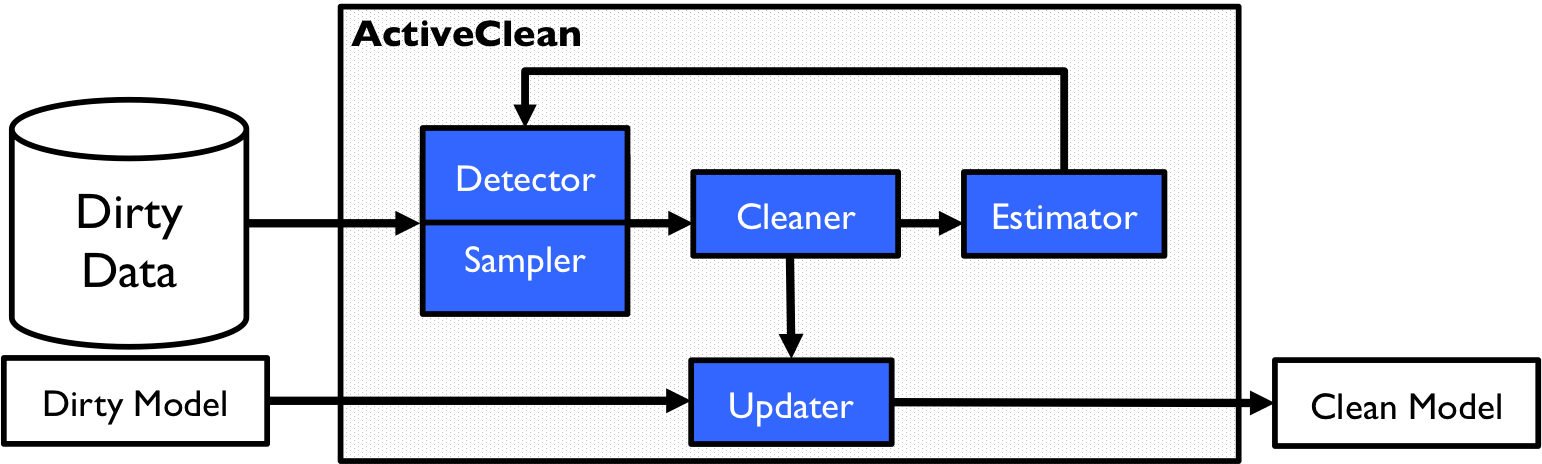
\includegraphics[width=\columnwidth]{figs/arch.png}
 \caption{\sysfull is an architecture where data cleaning is integrated with model training in a framework with sampling, model update, and feedback through estimation. \label{sys-arch}}\vspace{-2em}
\end{figure}

We propose \sys to address the progressive data cleaning problem in a way that avoids the three challenges: mixing, sampling, and sparsity.
The key insight is that an important class of predictive models, called convex loss models (e.g., linear regression and SVMs), are trained by iteratively drawing random samples of data and updating a model\cite{bertsekas2011incremental}.
Rather than happening before model training, Data cleaning can be directly integrated with the sampling and updating training process; preserving the same provable guarantees such as convergence and error bounds.
In \sys, data are cleaned in small random batches and the model is incrementally updated based on the results.
Similar to Active Learning, \sys selects the most valuable records to clean with higher probability, however, it applies a number of optimizations that exploit the data cleaning setting such as avoiding data that is expected to be clean, estimating of the effect of data cleaning for a record, and batching together updates from already cleaned data.
This framework is optimized for problems requiring expensive data cleaning.

The \sys architecture (Figure \ref{sys-arch}) consists of a \emph{detector}, \emph{sampler}, \emph{cleaner}, \emph{updater}, and \emph{estimator}.
The cleaner is an existing data cleaning framework (e.g., Entity Resolution), and \sys provides the remaining components to apply this framework progressively.
To summarize the contributions in each component:
\begin{itemize}[noitemsep]
\item Detector (Section \ref{det}). The detector can apply rules from data quality constraints or adaptively learn which records are dirty to increase the fraction of dirty records sampled.
\item Sampler (Section \ref{dist-samp}). We derive an optimal sampling distribution that minimizes the update variance (i.e., how different would the update be if another sample was drawn) which linearly improves an error bound on the convergence rate.
\item Updater (Section \ref{model-update}). The updater applies a weighted stochastic gradient descent step to the current best model. This update converges if all of the data is cleaned, and for batch size $b$ and iterations $T$, converges with rate $O(\frac{1}{\sqrt{bT}})$. 
\item Estimator (Section \ref{sampling}) The estimator applies a Taylor Series linearization to decouple changes in different features using knowledge about what is wrong with the data to better estimate the impact of an error.
\item The experiments evaluate these components on 4 datasets with real and synthetic corruption (Section \ref{eval}). The results suggest that indeed \sys is better suited for cleaning and model training when $k\ll N$. For a 5\%  systematic corruption, to achieve the same accuracy as a state-of-the-art Active Learning algorithm cleaning 1000 records, \sys cleans 55\% fewer records.
\end{itemize}







\section{Problem Setup}\label{background}

\subsection{Motivating Analysis Scenario}
Large dirty data are prevelant \cite{fortunearticle}, and we introduce an example of systematic corruption in publically available data. We present the following running example with our Dollars for Docs dataset (see Experiments, Section \ref{dfd-exp}):

\vspace{0.25em}

\noindent\textbf{Dollars for Docs. }
ProPublica has collected a dataset of corporate contributions to doctors for analysis of whether these contributions (negatively) affect research. 
The dataset has the following schema:
\begin{lstlisting}[mathescape,basicstyle={\scriptsize}]
Contribution(pi_speciality$\textrm{,}$ drug_name$\textrm{,}$ device_name$\textrm{,}$ corporation$\textrm{,}$ amount$\textrm{,}$ dispute$\textrm{,}$ status)
\end{lstlisting}

\noindent\texttt{pi\_speciality} is a textual attribute describing the speciality of the doctor recieving the contribution.

\noindent\texttt{drug\_name} is the branded name of the drug in the research study (null if not a drug).

\noindent\texttt{device\_name} is the branded name of the device in the study (null if not a device).

\noindent\texttt{amount} is a numerical attribute representing the contribution amount.

\noindent\texttt{dispute} is a boolean attribute describing whether the research was disputed.

\noindent\texttt{status} is a string label describing whether the contribution was covered under the declared research protocol. There are two statuses ``Covered" and ``Non-Covered".

\vspace{0.25em}

Using this dataset, consider the following analysis scenario.
\begin{example}
We are interested in predicting impropriety in medical research contributions, by exploring what features of a research contribution predict the \texttt{status} (i.e., not allowed in the protocol).
We featurize the textual attributes with a bag-of-words model and treat the \texttt{amount}/\texttt{dispute} attributes as numerical features.
The predictive model is a Support Vector Machine (SVM) that predicts the label $\{1,0\}$ where $1$ indicates a disallowed contribution.
\end{example}

In an ideal world, such a model would be robust to small corruption in the data.
However, the systematic nature of the corruption, can result in a misleading model.
On the Pro Publica website \cite{dollarsfordocs}, they list numerous types of corruption that had to be cleaned before publishing the data (see Appendix \ref{dfd-errors}).
For example, the most significant contributions were made by large companies whose names were also more often inconsistently represented in the data e.g. ``Pfizer Inc.", ``Pfizer Incorporated", ``Pfizer".
In a fraud detection scenario such as this one, the effect of systematic error can be serious.
Duplicate entity representations, could reduce the correlation between these entities and impropriety.

\vspace{0.25em}

\noindent\textbf{Cleaning With a Budget: }  Let us suppose our analyst wants evaluate whether the problems affect her model, and she wants to do this without having to manually validate every record. 
The first solution to this problem is to clean a sample of data, write this sample back, and then retrain the model on the partially cleaned data.
However, this solution can give unreliable results since we are mixing dirty and clean data.
In Figure \ref{update-arch1}, we illustrate the dangers of this approach on a very simple dirty dataset and model.
Suppose, we are trying to find a best fit line for two variables. 
One of the variables is systematically corrupted with a translation in the x-axis (Figure \ref{update-arch1}a).
We mark the dirty data in brown and the clean data in orange, and show their respective best fit lines in blue.
If we clean two of the data points (Figure \ref{update-arch1}b), and then find the best fit line, the partially cleaned model is dramatically incorrect.
This is a well-known phenomenon called Simpsons paradox, where mixtures of different populations of data can result in spurious relationships \cite{simpson1951interpretation}.
The result is surprising, namely, Machine Learning on partially cleaned data can lead to misleading results.

The next solution is avoiding the dirty data altogether.
She can take a sample of data, apply data cleaning, and train a model only on that sample of data.
This is similar to SampleClean \cite{wang1999sample}; proposed to approximate the results to aggregate queries by applying them to a clean sample of data.
Machine Learning models are highly senstive to sample size when high dimensional.
The result is that the models will not be useful (i.e., cannot accurately predict test data) when the sample size is too small (Figure \ref{update-arch1}c).

\begin{figure}[ht!]
\centering
 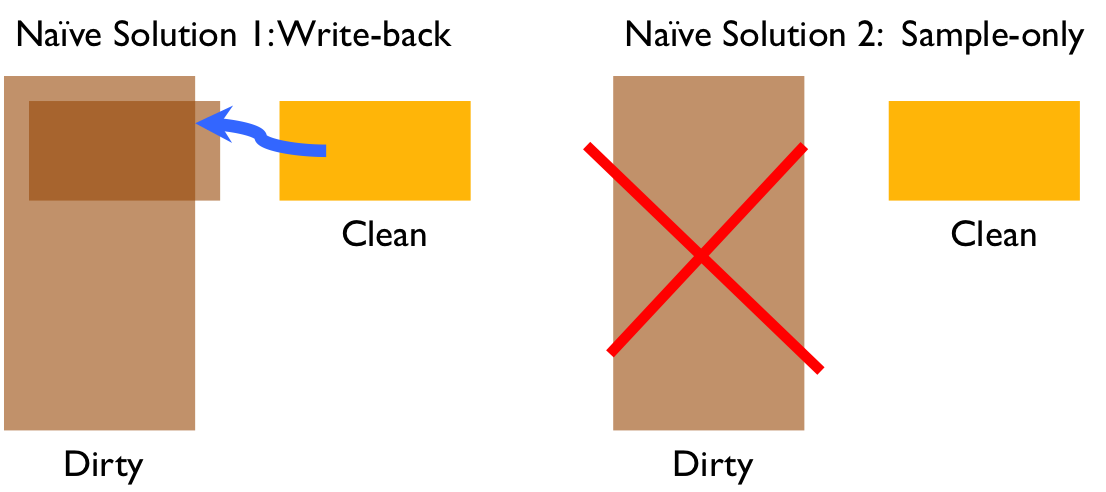
\includegraphics[width=\columnwidth]{figs/update-arch.png}
 \caption{(a) We present a dataset with a systematic corruption (translation) in one variable where the dirty data is in brown and the clean data is in yellow. If we draw the best fit line (i.e., linear regression), we see that the systematic corruption affects the line.
 (b) However, after cleaning two data points, applying the same model to partially clean data results in a dramatically incorrect answer.
(c) Likewise, small sample sizes can result in similarly incorrect models. \label{update-arch1}}
\end{figure}

\sys avoids both pitfalls, Simpsons's paradox and sample size dependence.
In Section \ref{model-update}, we show how we do this with iterative gradient steps (i.e., incrementally moving the line based on the clean data).
This takes advantage of the dirty data as well as the clean data, but still have provable properties about the intermediate results.
In Figure \ref{sys-arch2}, we illustrate our ideal tradeoff space of sampling and data cleaning.
At two extremes we have no cleaning (just using the dirty data) and full cleaning.
\sys is optimized for convergence for smaller sample sizes than a uniform sampling approach.

\begin{figure}[t]
\centering
 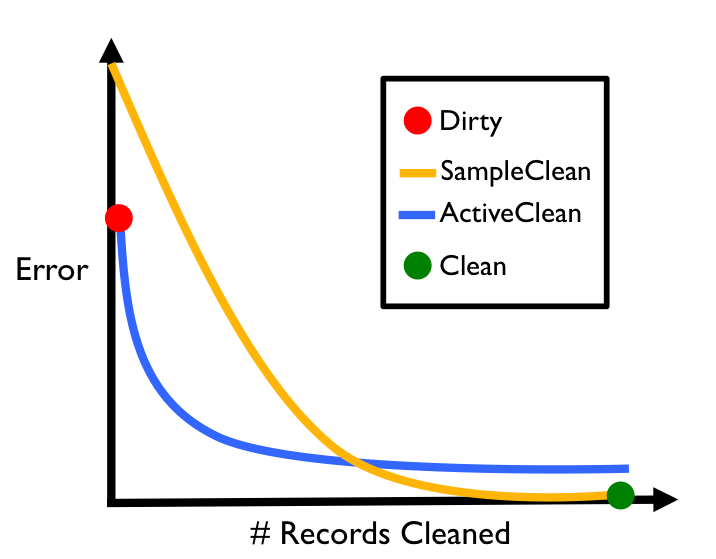
\includegraphics[width=0.5\columnwidth]{figs/arch2.png}
 \caption{Our goal with \sys is designed to converge to an accurate model with fewer cleaned records than a uniform sampling approach (SampleClean). \label{sys-arch2}}\vspace{-1em}
\end{figure}

\iffalse

We design \sys to make greater progress at these small sample sizes using the dirty model as an initialization.
Doing so is not trivial since it requires analysis of both the Machine Learning model and the data cleaning operations.
Data may look unimportant to a dirty model but when cleaned are very important.
Also, data cleaning and model training can happen at very different time scales, we have to carefully budget our effort to ensure that any optimizations actually address rate-determining steps in the workflow.
Finally, in this line of work, the tradeoff space is enormous, and we have to carefully pick a design point and tailor our optimizations to this preferred regime.
\fi

\subsection{Preliminaries}
\iffalse
There have been a few proposals of tighter integration of data cleaning and analytics.
In SampleClean \cite{wang1999sample}, the authors formalize the analytics in terms of a SQL aggregate query.
Bergman et al. explore the problem of query-oriented data cleaning \cite{bergman2015query}, where a conjunctive query (CQ) guides which records are to be cleaned.
SQL and CQ formalize a declarative problem specification in database research.
In a loose analogy to the declative queries in databases, loss functions in serve the same purpose in ERM.
\fi

We focus on a class of Supervised Learning problems called Empirical Risk Minimization (ERM) (see Friedman, Hastie, and Tibshirani \cite{friedman2001elements} for an introduction).
In ERM, the goal is to learn a set of model \emph{parameters} $\theta$ from training examples.
We start with a set of training examples $\{(x_{i},y_{i})\}_{i=1}^{N}$
on which we minimize a loss function $\phi$ (a penalty for getting the prediction wrong) at each point parametrized by $\theta$.
A very important class of problems is when the loss function is convex in $\theta$.
Convex problems are amenable to a variety of different optimization methodologies
and have strong theoretical guarantees on convergence rates.
This class of problems includes all generalized linear models (including linear and logistic regression), and all variants of support vector machines.
Formally,
\[
 \theta^{*}=\arg\min_{\theta}\sum_{i=1}^{N}\phi(x_{i},y_{i},\theta)
\]
For example, in a linear regression $\phi$ is:
\[
\phi(x_{i},y_{i},\theta) = \|\theta^Tx_{i} - y_i \|_2^2
\]
Typically, a \emph{regularization} term $r(\theta)$ is added to this problem.
$r(\theta)$ penalizes high or low values of feature weights in $\theta$ to avoid overfitting to noise in the training examples.
\[
 \theta^{*}=\arg\min_{\theta}\sum_{i=1}^{N}\phi(x_{i},y_{i},\theta) + r(\theta)
\]
For example, a popular variant of linear regression is called LASSO which is:
\[
 \theta^{*}=\arg\min_{\theta}\sum_{i=1}^{N}\|\theta^Tx_{i} - y_i \|_2^2 + \lambda \cdot \|\theta\|_1
\]
By applying the L1 regularization term, if one of the features is particularly noisy, and does not add predictive value, it will get excluded.
The loss function specifies a problem independent of the optimization used to calculate the optimal parameter $\theta^{*}$.

\subsubsection{Types of Errors}
When discussing ``errors" in Machine Learning models, we refer to the following metrics:

\vspace{0.25em}

\noindent\textbf{Model Error. } Let $\theta$ be the model trained on the dirty data, and let $\theta^*$ be the model trained on the same data if it were cleaned. Then the model error is defined as $\|\theta - \theta^*\|$.

\vspace{0.25em}

\noindent\textbf{Testing Error. } Let $\theta$ be the model trained on the dirty data, and let $\theta^*$ be the model trained on the same data if it were cleaned. Let $T(\theta)$ be the out-of-sample testing error when the dirty model is applied to the clean data, and $T(\theta^*)$ be the test error when the clean model is applied to the clean data. The testing error is defined as $T(\theta^*) - T(\theta)$

\vspace{0.5em}

\noindent The \emph{error} in the model and in testing is caused by two underlying problems:

\vspace{0.25em}

\noindent\textbf{Data Error. } Error caused by dirtiness.

\vspace{0.25em}

\noindent\textbf{Sampling Error. } Error introduced by sampling i.e., the difference between a model trained on $p\%$ of the data and $100\%$ of the data.

\vspace{0.25em}

In this paper, when we use the term \emph{error}, we are refering to \textbf{model error}.
We will be explicit when we are using the word error to describe problems regarding dirtiness in the underlying data (e.g. ``data corruption").

\subsection{\sys Problem}
The basic question that we explore in this work is how to update a model trained on dirty data with data cleaning. Formally,

\begin{problem}[ActiveClean Problem]\label{activeclean}\sloppy
Let $R$ be a dirty relation and each row $r \in R$ is 
turned into a feature vector and label tuple $F(r) \mapsto (x,y)$.
We are given a convex regularized loss model parametrized
by $\theta$ trained on the set of features and labels $\{(x,y)\}$.
The user specifies a data repair step which cleans a record 
$C(r) \mapsto r_{clean}$.
Optionally, the user can provide a set of dirty data detection conditions that select 
a set of candidate dirty data $R_{dirty}$.
With a budget of applying cleaning i.e., $C(\cdot)$, only k times, return an estimate $\hat{\theta}$ of the clean model.
\end{problem}

Our goal is to use information from the model to inform data cleaning on samples, and use the information from clean samples to update the model.
The tight feedback loop between model training and data cleaning poses several new algorithmic challenges. 
If we are not careful about how we update the model, we can end up with the Simpsons paradox problem described before.
Data cleaning and model training happen at very different time scales, we have to carefully budget our effort to ensure that optimizations address rate-determining steps in the workflow.

This framework is optimized around problems with expensive data cleaning.
As the complexity of dirtiness increases, so does the amount of computation and human-effort needed to resolve them.
The consequence is that automated repair is either not scalable or relies on greedy repairs that can be unreliable.
Increasingly, human effort is seen as valuable in data cleaning \cite{park2014crowdfill, wang2012crowder, gokhale2014corleone, wang1999sample}.
When humans are involved, per record latencies for data repair are orders of magnitude larger than the CPU time needed for model training.
We can compare recent results in data cleaning to a model training framework like CoCoA implemented on Spark \cite{jaggi2014communication}.
Per record, BigDansing, a highly optimized automated Spark-based data cleaning system is 15.5x slower than CoCoA\footnote{For CoCoA to reach a precision of 1e-3}.
Crowd based techiques like CrowdFill \cite{park2014crowdfill} and CrowdER \cite{wang2012crowder} are over 100,000x slower per record.

\noindent Here is an example application of \sys with our running example:
\begin{example}
The analyst first trains her SVM model on the dirty data ignoring the effects of the errors returning a model $\theta^{(d)}$.
She decides that she has a budget of cleaning $100$ records, and decides to clean the 100 records in batches of 10 (set based on how fast she can clean the data, and how often she wants to see an updated result).
She initializes \sys with $\theta^{(d)}$.
\sys samples an intial batch of 10 records.
She manually cleans those records by using the medical record source data.
After each batch, the model is updated with the most recent cleaning results $\theta^{(t)}$.
The model improves after each iteration.
After $t=10$ of cleaning, the analyst has an accurate model trained with 100 cleaned records but still utilizes the entire dirty data.
\end{example}

\iffalse

\subsection{Two perspectives on error}
When faced with such errors there are two contrasting perspectives from the Machine Learning and the Database communities.

\vspace{0.5em}

\noindent\textbf{Existing Database Literature. } 
Traditionally, cleaning is agnostic to the queries and analysis that happens downstream. 
This perspective breaks down when cleaning is so expensive that we can only clean a small number of records.
Ideally, we should clean the records that are most valuable to the downstream analysis.

\vspace{0.5em}

\noindent\textbf{Existing  Machine Learning Literature. } The Machine Learning community has focused on
designing models that are robust to outliers (i.e., values far away from the typical value)
For example, in the case of linear regression, we can change the $L_2$ norm to an $L_1$ norm to mitigate the effect of outliers:
\[
\phi(x_{i}^T\theta,y_{i}) = \|\theta^Tx_{i} - y_i \|_1
\]
The quadratic L2 loss implies that examples that deviate far from the typical example are quadratically penalized as opposed to linearly penalized with the L1 loss.
There is a natural tradeoff between robustness and efficiency.
The more robust a technique is, the less efficient it will be (i.e., estimate variance for a fixed number of training examples).
Robust techniques are best suited for random errors that look significantly different the rest of the examples.
When errors are systematic, the Machine Learning answer has been to design features in such a way that they are robust to some systematic bias.
For example, in image processing, scale-invariant feature transforms (SIFT) are widely applied that allow for image models invariant to pose or scaling issues.

\vspace{0.5em}

\noindent\textbf{The \sys Contribution. } We try to bring two perspectives together in this work to address the problem of expensive to clean systematic errors, namely the Database idea of data cleaning and the Machine Learning formalization of empirical risk minimization.
Some errors require expensive cleaning procedures, increasingly using the crowd, and we joint have a time budget on cleaning and analysis.
\sys prioritizes cleaning with respect to an estimated impact on the clean model.



\subsection{SampleClean Project}

Traditionally, data cleaning has explored expensive, up-front cleaning of entire datasets for increased query accuracy.
We proposed the SampleClean problem, in which an analyst cleans a small sample of data, and then estimates the result to an aggregate query e.g., \sumfunc, \countfunc, or \avgfunc.
The main insight from the SampleClean project is that highly accurate answers for aggregate queries does not require cleaning the full dataset.
Generalizing this insight, there is a deep relationship between the application (i.e., the query) and how an analyst should budget their effort in data cleaning.
In fact, \avgfunc and \sumfunc queries are a special case of the convex loss minimization discussed in the previous section:
\[
\phi = (x_{i} - \theta)^2
\]

We then extended the SampleClean work to study cleaning Materialized Views \cite{technicalReport}.
Suppose base data is updated with insertions, deletions, or updates, we explored how we could efficiently propagate
changes to a sample of the view instead of the full view.
Subsequent queries on the view could be answered approximate.

The SampleClean problem inspired an eponymous system that implements sampling, data cleaning, and approximate query processing on the Apache Spark stack \cite{sampleclean}.
Also included in the Apache Spark stack are Machine Learning libraries including MLlib \cite{mllib} and GraphX \cite{graphx}.
The in-memory architecture of the Apache Spark stack allows for increasingly interactive analysis \cite{AgarwalMPMMS13, armbrust2015spark}.
Analysts can prototype data processing workflows on samples to evaluate performance before running expensive batch processing jobs on entire datasets.
With data cleaning and machine learning libraries in the same software ecosystem, we see a new opportunity for joint optimization for interactive model building.



\subsection{Stochastic Gradient Descent}
Sampling is a natural part of any Machine Learning workflow, as stochastic optimization is widely used to fit model parameters.
The problems described in the previous subsections are often trained using a technique called Stochastic Gradient Descent (SGD) or one of its variants.
The basic idea of SGD is to draw a data point at random, calculate the gradient at that point, and then update a current best estimate with that gradient.
\[
\theta^{(t+1)}\leftarrow\theta^{(t)}-\gamma\nabla\phi(x_{i}^T\theta,y_{i})
\]
 SGD can also be applied in a ``mini-batch" mode, where we draw a subset of data $S^{(t)}$ at random and update with the average gradient.
 \[
 \theta^{(t+1)}\leftarrow\theta^{(t)}-\frac{\gamma}{\|S^{(t)}\|}\sum_{i\in S^{(t)}}\nabla\phi(x_{i}^T\theta,y_{i})
 \]

We can use this workflow for designing an anytime data cleaning methodology.
As data is sampled, we can clean the samples.
The analyst then can stop at anytime and use the best model at that instant.
SGD and its variants are well-studied and there are lower-bounds on the convergence rates using these techniques. 
Recently, a number of works have explored non-uniform sampling distributions for stochastic optimization \cite{zhao2014stochastic, qu2014randomized}.
The main insight is that non-uniform distributions may on average estimate the gradient accurately.
In this work, we explore how to design such a non-uniform distribution for iterative data cleaning.

\fi


 
\section{System Architecture}\label{arch}
This section describes the \sys architecture and the basic algorithmic framework.
The individual components will be addressed in the subsequent sections.

\subsection{Overview}
Figure \ref{sys-arch}, in the introduction, overviews the entire framework.
The first step of \sys is \emph{initialization}.
In this step, there is a dirty relation $R$, a featurization $F(\cdot)$, a data cleaning technique $C(\cdot)$, and a dirty model $\theta^{(d)}$ trained on the featurized dirty relation. 
Optionally, \sys integrates with dirty data detection rules $D(\cdot)$ which selects the set of likely corrupted records from $R$.
If one is not provided, \sys starts by treating all of the data as dirty and tries to learn a detector as data are cleaned.
At initialization, there are two hyperparameters to set, the cleaning budget $k$ and the batch size $b$ (the number of iterations is $T = \frac{k}{b}$).
We discuss how to set $b$ and the tradeoffs in setting a larger or smaller $b$ in Section \ref{model-update}.

After initialization, \sys begins the cleaning and model update iterations.
The \emph{sampler} selects a sample of dirty data based on the batch size.
At this step, \sys can use the detector $D$ to narrow the sample to likely dirty data.
Once a sample is selected, the \emph{cleaner} applies $C(\cdot)$ to the dirty sample.
%Then, after the sample is cleaned, the current model is updated.
\sys is initialized with the dirty model, and this model is iteratively updated as more batches are cleaned.

The next two steps in the architecture are feedback steps where the sampling distribution is updated for the next iteration.
The \emph{estimator} uses previously cleaned data to estimate the value of data cleaning on new records.
This information is used to guide sampling towards more valuable records.
After estimation, the detector $D(\cdot)$ is also updated based on cleaned data.
After all of the iterations are complete, the system returns the updated model.

To summarize the architecture in pseudocode:
\begin{enumerate}[leftmargin=1em]\scriptsize\sloppy
\item \texttt{Init(dirty\_data, cleaned\_data, dirty\_model, batch, iter)}
\item For each t in $\{1,...,T\}$
\begin{enumerate}
	\item \texttt{dirty\_sample $=$ Sampler(dirty\_data, sample\_prob, detector, batch)}
	\item \texttt{clean\_sample $=$ Cleaner(dirty\_sample)}
	\item \texttt{current\_model $=$ Update(current\_model, sample\_prob, clean\_sample)}
	\item \texttt{cleaned\_data = cleaned\_data + clean\_sample}
	\item \texttt{dirty\_data = dirty\_data - clean\_sample}
	\item \texttt{sample\_prob $=$ Estimator(dirty\_data, cleaned\_data, detector)}
	\item \texttt{detector $=$ DetectorUpdater(detector, cleaned\_data)}
\end{enumerate}
\item \texttt{Output: current\_model}
\end{enumerate}

Here is an example application of \sys:
\begin{example}
The analyst first trains an SVM model on the dirty data ignoring the effects of the errors resulting in a model $\theta^{(d)}$.
She decides that she has a budget of cleaning $100$ records, and decides to clean the 100 records in batches of 10 (set based on how fast she can clean the data, and how often she wants to see an updated result).
She initializes \sys with $\theta^{(d)}$.
\sys samples an initial batch of 10 records.
She manually cleans those records by merging similar drug names, making corporation names consistent, and fixing incorrect labels.
After each batch, the model is updated with the most recent cleaning results $\theta^{(t)}$.
The model improves after each iteration.
After $t=10$ of cleaning, the analyst has an accurate model trained with 100 cleaned records but still utilizes the entire dirty data.
\end{example}

\subsection{Challenges and Formalization}
We highlight the important components and formalize the research questions explored in this paper. 

\vspace{0.5em}

\noindent\textbf{Detector (Section \ref{det}). } The first challenge in \sys is dirty data detection. In this step, the detector select a candidate set of dirty records $R_{dirty} \subseteq R$. There are two techniques to do this: (1) an \emph{a priori} case, and (2) and an adaptive case. In the \emph{a priori} case, the detector knows which data is dirty in advance. In the adaptive case, the detector learns classifier based on previously cleaned data to detect corruption in uncleaned data.

\vspace{0.5em}

\noindent\textbf{Sampler (Section \ref{dist-samp}). } The sampler draws a sample of records $S_{dirty} \subseteq R_{dirty}$. This is a non-uniform sample where each record $r$ has a sampling probability $p(r)$.
We will derive the optimal sampling distribution, and show how the theoretical optimal can be approximated by the next estimator.

\vspace{0.5em}

\noindent\textbf{Cleaner (User-Specified). } Given the sample of the records $S_{dirty}$,  the cleaner applies the user-specified data cleaning $C(\cdot)$. This paper focuses on a record-by-record cleaning model where the function $C$ is applied to a record and produces the clean record:
\[
S_{clean} = \{C(r) : \forall r \in S_{dirty}\}
\]
This allows for uniform measure of the performance of \sys in terms of model error as a function of sample size. The record-by-record cleaning model is not a fundamental restriction of this approach, and in the extensions (Section \ref{set-of-r}), there is a discussion on a compatible ``set of records" cleaning model. Consider the case where an analyst finds a dirty record, and is able to fix all records (possibly outside the sample) the with same error throughout the dataset efficiently.

\vspace{0.5em}

\noindent\textbf{Update (Section \ref{model-update}). } This step updates the model $\theta^{(t)}$ based on the featurized (with featurization $F(\cdot)$) cleaned sample $F(S_{clean})$ resulting in $\theta^{(t+1)}$. Analyzing the model update procedure as a stochastic gradient descent algorithm will help derive the sampling distribution and estimation.

\vspace{0.5em}

\noindent\textbf{Estimator (Section \ref{sampling}): } The estimator approximates the optimal distribution derived in the Sample step. Based on the change in the featurized data $F(S_{clean})$ and $F(S_{dirty})$, it directs the next iteration of sampling to select points that will have changes most valuable to the next model update.

\iffalse
\subsection{Optimizations}
There are three aspects of \sys, that allow us to achieve this design point: error partitioning, gradient-based model update (Section \ref{model-update}), estimate-driven sampling (Section \ref{sampling}).

\vspace{0.5em}

\noindent\textbf{Partitioning Dirty and Clean Data: } In many applications, enumerating the set of corrupted records is much easier than cleaning them. For example, we may be able to select the set of rows that have missing values but actually filling those missing values is expensive. Likewise, in the constraint literature, selecting a set of rows that have a violated constraint can be done in polynomial time, however, fixing the constraints is NP-Hard.
In our error detection step, we partition the dirty and clean data.
Partitioning serves two purposes: (1) it reduces the variance of our updates because we can cheaply scan over data we know that is clean, and (2) it increases the fraction of actually dirty records in the candidate batch.
A good example of why we need the second objective is seen in the context of crowdsourcing.
If we have a crowdworker clean records, we will have to pay them for the task whether or not the record required cleaning.
To efficiently use this partitioning, we need a database solution indexing dirty and clean data.

\vspace{0.5em}

\noindent\textbf{Gradient-Based Updates: } In \sys, we start with a dirty model and then make an update using a gradient step. Here, we can draw an analogy to Materialized View maintenance, since after all, a model parametrized by $\theta$ is just a table of floating point numbers.
Krishnan et al. proposed a technique called sample view cleaning, in which they take a clean sample of data and propagate the updates to a Materialized View.
Similarly, in this work, we take the information from a sample of cleaned data and propagate an update with the gradient.

\vspace{0.5em}

\noindent\textbf{Estimate-Driven Sampling: } Repair is the most expensive step in the workflow, so optimizing for scan cost may lead to negligible overall time improvements.
We can sacrifice a small overhead in pre-computation for each data point to determine its value to the model and select a sampling distribution accordingly.
Intuitively, while each iteration has an increased cost, it also makes more progress towards the optimum.
\fi



\section{Detection}\label{det}
To maximize the benefit of data cleaning, detection ensures that sampling draws records likely to be dirty.

\subsection{Goals}
The detector returns two important aspects of a record: (1) whether the record is dirty, and (2) if it is dirty, what is wrong with the record.
The sampler can use (1) to select a subset of dirty records to sample at each batch. 
The estimator can use (2) estimate the value of data cleaning based on other records with the same corruption.
\sys supports two types of detectors \emph{a priori} and \emph{adaptive}.
In the \emph{a priori} case, there is a way to select the set of dirty records before any cleaning.
This case is possible for some types of data errors.
In the adaptive case, detection is learned as data is cleaned.

\subsection{A Priori Case}
For many types of dirtiness such as missing attribute values and constraint violations, it is possible to efficiently enumerate a set of corrupted records and what is wrong with them.

\begin{definition}[A Priori Detection]
Let $r$ be a record in $R$. An a priori detector is a detector that returns a Boolean of whether the record is dirty and a set of columns $e_r$ that are dirty.
\[
D(r) = (\{0,1\}, e_r)
\]
From the set of columns that are dirty, find the corresponding features that are dirty $f_r$ and labels that are dirty $l_r$.
\end{definition}

\noindent Here are example use cases of this definition using data cleaning methodologies proposed in the literature.

\vspace{0.5em}

\noindent\textbf{Constraint-based Repair: }
One model for detecting errors involves declaring constraints on the database.

\vspace{0.5em}

\emph{Detection. } Let $\Sigma$ be a set of constraints on the relation $\mathcal{R}$. 
In the detection step, the detector select a subset of records $\mathcal{R}_{dirty} \subseteq \mathcal{R}$ that violate at least one constraint.
The set $e_r$ is the set of columns for each record which have a constraint violation. 

\begin{example}
An example of a constraint on the running example dataset is the \texttt{status} of
a contribution can be only ``allowed" or ``disallowed".
Any other value for \texttt{status} is an error.
\end{example}

\vspace{0.5em}

\noindent\textbf{Entity Resolution: }
Another common data cleaning task is Entity Resolution \cite{gokhale2014corleone, DBLP:journals/pvldb/KopckeTR10, wang2012crowder}.
Entity Resolution is the problem of standardizing attributes that represent the same real world entity.
A common pattern in Entity Resolution is to split up the operation into two steps: blocking and matching.
In blocking, attributes that should be the same are coarsely grouped together.
In matching, those coarse groups are resolved to a set of distinct entities.

\vspace{0.5em}

\emph{Detection. } Detection for entity resolution problems is the matching step. Let $S$ be a similarity function that takes two records and returns a value in $[0,1]$ (1 most similar and 0 least similar). For some threshold $t$, $S$ defines a similarity relationship between two attributes $r(a)$ and $r'(a)$:
\[
r(a) \approx r'(a) : S(r(a),r'(a)) \ge t
\] 
In the detection step, $R_{dirty}$ is the set of records that have at least one other record in the relation that satisfies $r(a) \approx r(a)'$.
The set $e_r$ is the set of attributes of $r$ that have entity resolution problems.

\begin{example}
An example of an Entity Resolution problem is seen in our earlier example about corporation names e.g. ``Pfizer Inc.", ``Pfizer Incorporated", ``Pfizer".. 
Given a similarity relationship $WeightedJaccard(r1,r2)>0.8$, the detector selects all records that satisfy this condition (their Weighted Jaccard Similarity is greater than 0.8).
\end{example}

\subsection{Adaptive Detection}
\emph{A priori} detection is not possible in all cases.
The detector also supports adaptive detection where detection is learned from previously cleaned data.
Note that this ``learning" is distinct from the ``learning" at the end of the pipeline.
The challenge in formulating this problem is that detector needs to describe how the data is dirty (e.g. $e_r$ in the \emph{a priori} case).
The detector achieves this by categorizing the corruption into $u$ classes.
These classes are corruption categories that do not necessarily align with features, but every records is classified with at most one category.
For example, suppose there are records with outliers and missing values, there are three classes of corruption: outliers, missing values, and both.

When using adaptive detection, the repair step has to clean the data and report to which of the $u$ classes the corrupted record belongs.
When an example $(x,y)$ is cleaned, the repair step labels it with one of the ${\text{clean}, 1,2,...,u+1}$ classes (including one for ``not dirty").
It is possible that $u$ increases each iteration as more types of dirtiness are discovered. 
Then, the detection problem reduces to a multiclass classification problem.
This problem can be addressed by any multiclass classifier, and we use an all-versus-one SVM in our experiments.
Since this classifier is internal to our system, it does not have to be a convex model (i.e., it can be a Decision Tree or Random Forest).

\begin{definition}[Adaptive Case]
Select the set of records for which $\kappa$ gives a positive error classification (i.e., one of the $u$ error classes).
After each sample of data is cleaned, the classifier $\kappa$ is retrained.
So the result is:
\[D(r) = (\{1,0\},\{1,...,u+1\})\]
\end{definition}

\vspace{0.75em}

\noindent\textbf{Adaptive Detection With Open Refine: }
\begin{example}
OpenRefine is a spreadsheet-based tool that allows users to explore and transform data.
However, it is limited to cleaning data that can fit in memory on a single computer.
Since the cleaning operations are coupled with data exploration, \sys does not know what is dirty in advance (the analyst may discover new errors as she cleans).

Suppose the analyst wants to use OpenRefine to clean the running example dataset with \sys.
She takes a sample of data from the entire dataset and uses the tool to discover errors.
For example, she finds that some drugs are incorrectly classified as both drugs and devices.
She then clears the device attribute for all records that have the drug name in question.
Every time she makes a batch data transformation (i.e., cleaning the device attribute), \sys can list the set of records that have changed.
Each transformation becomes and error class, and the records that have changed records become positive training examples for a classifier to guide future samples.
\end{example}
\section{Update}\label{model-update}
Before we discuss sampling, we will first discuss how to update a model.
We will assume that our detection step in the previous section has selected 
a set of candidate records $R_{dirty}$ and our sampling step has sampled from this
set of candidate records.
We will show that this model update procedure can be interpreted as a Stochastic 
Gradient Descent (SGD) algorithm, which gives us a theoretical framework to analyze
convergence and bound the error at each step.

\subsection{Update Problem}
The high level challenge is that we want a model update technique that takes advantage of the entire dirty data and a small sample of cleaned data.
We want this technique to have some provable guarantees like the conditions under which we converge to the right answer as the entire data is cleaned, bounds on error of intermediate results, and a guarantee that cleaning will improve the error.  

First, let us describe the abstract problem.
Suppose we have a cleaned batch of data $S_{clean}$ with features and labels $(X_{clean},Y_{clean})$, and a dirty model $\theta^{(d)}$. 
In the model update problem, we update the dirty model with some function $f(\cdot)$ i.e.,:
\[
\theta^{new} \leftarrow f(X_{clean},Y_{clean},\theta^{(d)})
\]
Our goal is that these updates should minimize the error of the updated model and the true model $\theta^{(c)}$ (if we cleaned and trained over the entire data):
\[
error(\theta^{new}) = \| \theta^{new} - \theta^{(c)} \|
\]

There are a couple of challenges that we address in this section.
As described in our architecture, we do not want to clean data that we have already cleaned or is expected to be clean.
This leads to our first challenge since the sample $S_{dirty}$ may not be representative of the full data, only $R_{dirty}$. 
We have to design our update in such a way that it does not bias our result towards the newly cleaned data. 
The second challenge is that we need to get the sample $S_{dirty}$ from $R_{dirty}$.
Some records, if cleaned, are more informative than others.
We show how to incorporate non-uniform sampling into our update and formulate the theoretical optimal sampling problem.
In the next section, we will discuss how to practically address the optimal sampling problem.

\subsection{The Geometry Of The Problem}
Let us try to understand the geometry of this problem in one dimension (i.e., the parameter $\theta$ is a scalar vale).
We restrict the class of Machine Learning models to convex regularized loss problems.
That is, as we vary the model $\theta$ the loss is bowl-shaped (visualized in Figure \ref{update-arch2}a).
There is a unique optimal value for $\theta$ at the bottom of the bowl.
If we have dirty data, we are training a model with respect to an incorrect data distribution.
In other words, we are optimizing the wrong function (Figure \ref{update-arch2}b).
The resulting dirty model can be thought of as a suboptimal point on clean curve.

\begin{figure}[ht!]
\centering
 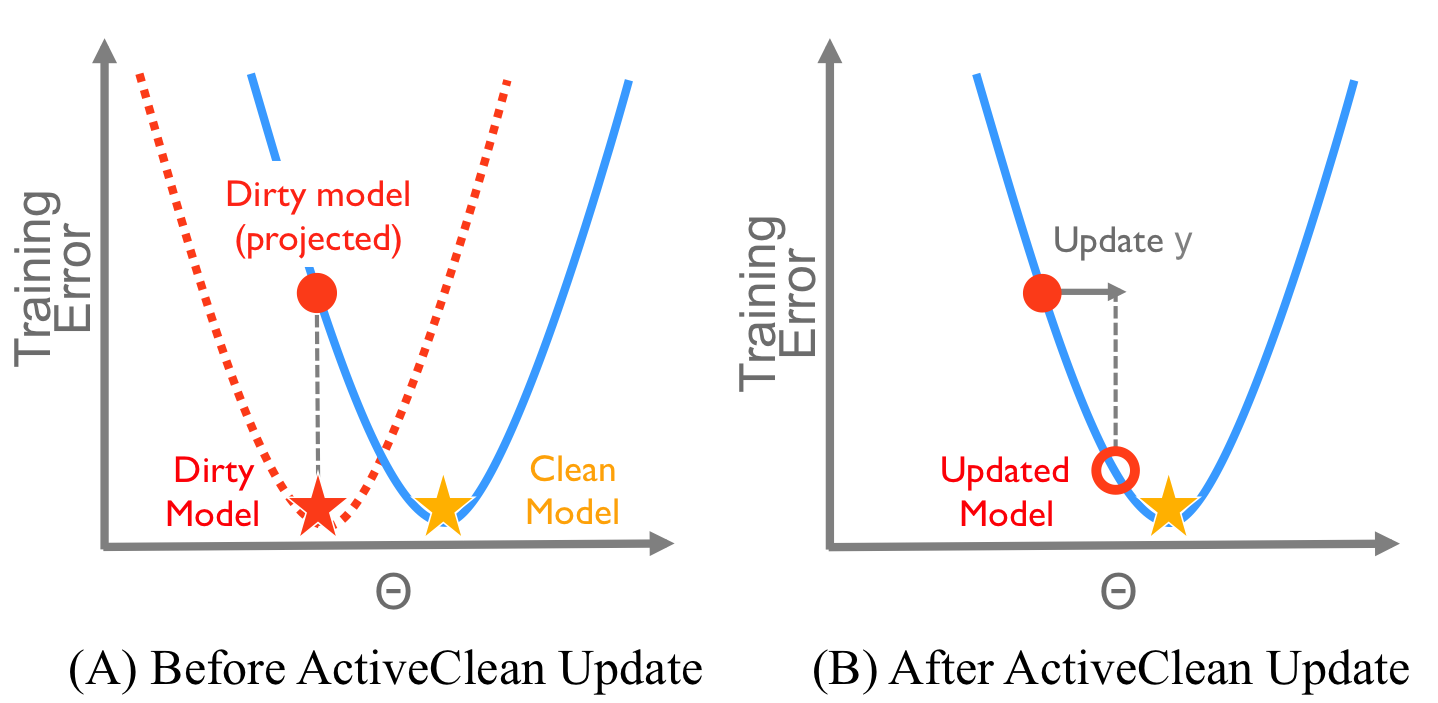
\includegraphics[width=\columnwidth]{figs/update-arch2.png}
 \caption{In \sys, we explore an important class of Machine Learning problems where the loss function (i.e., training error) varies convexly. An incorrect model can be thought of as a sub-optimal point. \label{update-arch2}}
\end{figure}

We have a model $\theta^{(d)}$ (visualized in brown) that is suboptimal with respect to the clean data.
We want to get to the optimal clean model $\theta^{(c)}$ which is visualized as a yellow star.
If we had all of the clean data we could compute $\theta^{(c)}$.
However, at each iteration, we only have a sample of clean data.
To resolve this issue, we can exploit the model's geometry.
For this class of models, given a suboptimal point, we can find the direction to the 
the global optimum.
Mathematically, this direction corresponds to gradient of the loss with respect to $\theta$, and we need to move some distance $\gamma$ along this direction:
\[
\theta^{new} \leftarrow \theta^{(d)} - \gamma \cdot \nabla\phi(\theta^{(d)})
\]
In our visualization, this corresponds to whether we should move left or right.
The intuition, which we will formalize in Section \ref{sgd}, is that if we are on average in the right direction the algorithm is guaranteed to converge with analytics bounds on the convergence rate.
At the optimal point, the expected gradient will be zero.
So intuitively, this approach iteratively moves the model downhill, or corrects, the dirty model until the budget is reached.

\subsection{Average Gradient From a Sample}
Our class of Machine Learning models are based on loss minimization, that is they are a sum of losses, and we know that sums commute with derivatives.
So to calculate the average gradient from a sample, we simply calculate the gradient at every data point and average over them.
Let $S$ be a sample of data, where each $i \in S$ is drawn with probability $p_i$.
We can approximate the global gradient:
\[
\nabla\phi(\theta) \approx g_{S}(\theta) = \frac{1}{n\mid S \mid} \sum_{i \in S}\frac{1}{p_i}\nabla\phi(x_i^{clean},y_i^{clean},\theta)
\]
Then for every batch of data cleaned, we apply the update to the current best model estimate:
\[
\theta^{(t)} \leftarrow \theta^{(t-1)} - \gamma \cdot g_{S}(\theta^{(t-1)})
\]

The tricky part is that only a subset of the records are are cleaned.
The consequence of this is that the estimate $g_{S}(\theta)$ is now biased.
We also have to compensate for this bias by averaging this estimate with the gradient with respect to the clean data:
\[
g_C(\theta) = \frac{1}{\mid R - R_{dirty}\mid}\sum_{i \in R - R_{dirty}}\nabla\phi(x_i^{clean},y_i^{clean},\theta)
\]
Then, for weights $\alpha,\beta$ which we will subsequently discuss how to select:
\[
g(\theta) = \alpha \cdot g_C(\theta) + \beta \cdot g_S(\theta)
\]
So then our final gradient update becomes:
\[
\theta^{(t)} \leftarrow \theta^{(t-1)} - \gamma \cdot g(\theta) \blacksquare
\]

\subsection{Model Update Algorithm}
Following from this geometric analysis, we propose the iterative model correction algorithm.
We initialize the algorithm with $\theta^{(d)}$ which is the dirty model.
At each iteration $i=\{1,...,t\}$, we clean a batch of data $b$ selected from the set of candidate dirty records $R_{dirty}$.
Then, starting with $\theta^{(d)}$, we apply an averaged gradient update to get $\theta^{(i)}$.
We iterate until our budget of cleaning $k = t \cdot b$ record is reached.

We present the model update algorithm here:
\begin{enumerate}[noitemsep]
	\item Calculate the gradient over the sample of clean data and call the result $g_S(\theta^{(i-1)})$
	\item Calculate the average gradient over all the data in $R_{clean}$, and call the result $g_C(\theta^{(i)})$
	\item Apply the following update rule:
	\[
	\theta^{(i+1)} \leftarrow \theta^{(i)} - \lambda \cdot(\alpha\cdot g_S(\theta^{(i)}) + \beta \cdot  g_C(\theta^{(i)}))
	\]
\end{enumerate} 

\subsubsection{Selecting the Parameters}
The proposed update policy makes intuitive sense.
However, we have still have to set the parameters $\lambda$, $\alpha$, $\beta$.
We will show that theory from the stochastic optimization literature can allow us to understand this iterative algorithm.
First, we will review all of the parameters that need to be set.

\vspace{0.5em}

\noindent\textbf{Step Size $\gamma$ : } The first problem is that we have not explained how to pick the step size $\gamma$. In other words, how far should we travel in the gradient direction.

\vspace{0.5em}

\noindent\textbf{Step Size $\alpha,\beta$ : } The next problem is deriving the proportions with which we should combine $g_S(\theta)$ and $g_C(\theta)$. It turns out that $\alpha = \frac{R_{clean}}{R}$ and $\beta = \frac{R_{dirty}}{R}$, and we will show a derivation below.

\vspace{0.5em}

\noindent\textbf{Choosing $S$: } As we mentioned, the optimal clean model depends on \emph{all} the clean data, not just a sample. 
So $g_S$ is really an approximation of the the true gradient $g^*$ with some error $g^* \pm \epsilon$. 
The quality of the update depends on how well we can approximate $g^*$ using $g_S$.
The problem is how should we construct the sample of data to clean $S$ to get the most accurate update.
In particular, how should we choose the sampling probabilities $p_i$ for each $i \in S$ such that the error is minimized.

\subsection{Analysis with Stochastic Gradient Descent}\label{sgd}
This update policy can be formalized as a class of very well studied algorithms called Stochastic Gradient Descent.
This gives us a theoretical framework to understand and analyze our update rule, bound the error, and choosing points to clean.
Mini-batch stochastic gradient descent (SGD) is an algorithm for finding the optimal value
of $\theta$, given the convex loss, and data.

\vspace{0.5em}

\noindent\textbf{ Setting $\gamma$: } There is extensive literature in machine learning for choosing $\gamma$ appropriately. $\gamma$ can be set either to be a constant or decayed over time. Many machine learning frameworks (e.g., MLLib, Sci-kit Learn, Vowpal Wabbit) automatically set learning rates or provide different learning scheduling frameworks. 
In our experiments, we use a technique called inverse scaling where there is a parameter $\gamma_0=0.1$, and at each iteration we reduce it to $\gamma_t = \frac{\gamma_0}{\mid S \mid t}$. 

\vspace{0.5em}

\noindent\textbf{ Convergence: } The next property of concern is convergence. Convergence properties of batch SGD formulations has been well studied \cite{dekel2012optimal}. 
The conditions on this convergence are essentially that at each step the estimate of the gradient $g_S$ has to be unbiased, that is on average correct. 

\begin{proposition}
For an appropriately chosen learning rate $\gamma_t$, batch stochastic gradient descent will converge if $\mathbb{E}(g_S)=g^*$.
\label{unbiased}
\end{proposition}

A direct result of convergence is a guarantee on statistical consistency.
Another interesting consequence of this result is that we can sample $S$ in any way that we want
as long as our estimate in unbiased.

\vspace{0.5em}

\noindent\textbf{ Convergence Rate: } The convergence rates of SGD are also well analyzed \cite{dekel2012optimal,bertsekas2011incremental,zhao2014stochastic}. 
Suppose, a user cleans a batch size of $b$ examples at each iteration.
This allows us to bound the error of intermediate models and understand the expected number of steps before a model within a certain error. 

\begin{proposition}
For a general convex loss, a batch size $b$, and $t$ iterations, the convergence rate is bounded by $O(\frac{\sigma^2}{\sqrt{bt}})$. 
$\sigma^2$ is the variance in the estimate of the gradient at each iteration:
\[
\mathbb{E}(\|g_S - g^*\|^2)
\]
\end{proposition}

There is an interesting tradeoff between batch size an convergence rate.
Increasing the batch size reduces the variance $\sigma^2$, however it does
mean at each iteration you are doing more work.
In a data cleaning context, this is a problem since the bottlneck is the work at 
each iteration not the number of iterations.

\vspace{0.5em}

\noindent\textbf{ Laziness Argument: } The convergence and the error bounds show that the technique is theoretically justified, but the remaining question is whether the constant factors make this technique practical.
It is well known that even for arbitrary initializations SGD makes significant progress in less than one epoch (a pass through the entire dataset) \cite{bottou2012stochastic}.
In our case, we often have a decent initialization which is the dirty model, which means that we can get close processing far less than the full data.
Our algorithm is essentially an arguement for lazy materialization, where we only clean the data when needed.


\section{Selecting Records to Clean}\label{dist-samp}
The algorithm proposed in Section \ref{update-alg} will convege for 
any sampling distribution where  $p(\cdot) > 0$ for all records, albeit different distributions will have different convergence rates.
The sampling algorithm is designed to include records in each batch that are most valuable to the analyst's model with a higher probability.

\subsection{Optimal Sampling Problem}
Recall that the convergence rate of an SGD algorithm is bounded by $\sigma^2$ which is the variance of the gradient.
Intuitively, the variance measures how accurately the gradient is estimated from a uniform sample.
Other sampling distributions, while preserving the same expected value, may have a lower variance.
Thus, the optimal sampling problem is defined as a search over sampling distributions to find the minimum variance sampling distribution.

\begin{definition}[optimal Sampling Problem]
Given a set of candidate dirty data $R_{dirty}$, $\forall r \in R_{dirty}$ find sampling probabilities $p(r)$ such that over all samples $S$ of size $k$ it minimizes the variance:
\[
\arg\min_p \mathbb{E}(\|g_S - g^*\|^2)
\]
\end{definition}

It can be shown~\cite{zhao2014stochastic} that the optimal distribution over records in $R_{dirty}$ is proportional to: $p_i \propto \|\nabla\phi(x^{(c)}_i,y^{(c)}_i,\theta^{(t)})\|$
Intuitively, this sampling distribution prioritizes records with higher gradients, i.e., make a larger impact during optimization.
The challenge is that this particular optimal distribution depends on knowing the clean value of a records, which is a chicken-and-egg problem:
the optimal sampling distribution requires knowing $(x^{(c)}_i,y^{(c)}_i)$; however, we are sampling the values so that they can be cleaned.

One natural solution is to calculate this gradient with respect to the dirty values--implicitly assuming that the corruption is not that severe:
\[
p_i \propto \|\nabla\phi(x^{(d)}_i,y^{(d)}_i,\theta^{(t)})\|
\]
This solution is highly related to the Expected Gradient Length heuristic that has been proposed before in Active Learning\cite{settles2010active}.
However, there is additional structure to the data cleaning problem.
As the analyst cleans more data, we can build a model for how cleaned data relates to dirty data.
By using the detector from the previous section to estimate the impact of data cleaning, we show that we can estimate the cleaned values.
We find that this optimization can improve the convergence rate by a factor of 2 in some datasets.
%Note that as long as every record gets sampled, the algorithm will still converge.





\section{Estimation}\label{sampling}
In this section, we make the sampling result of the previous section practical,
and estimate the cleaned data.

\subsection{Challenges and Goal}
The optimal sampling distribution is dependent on a value that we cannot know without data cleaning $\nabla\phi(x^{(c)}_i,y^{(c)}_i,\theta^{(t)})$.
One way to approximate this distribution is to learn a function $e(\cdot)$ via regression based on the data that we have cleaned.
This is a high-dimensional regression problem which may have to learn a very complicated relationship between dirty and clean data.
The biggest challenge with such an estimator is the cold start problem, where if we have cleaned a small amount of data, the estimator will be inaccurate.
In \sys, we want to be able to make as much progress as possible in the early iterations so this technique may not work.
We take an alternative approach, where we try to exploit what we know about data cleaning to produce an estimate for groups of similarly corrupted records.
To define ``similarly corrupted", we are going to show how we can use the detection step to make this problem tractable.

\subsection{Estimation For A Priori Detection}
\begin{example}
Suppose records from running example dataset are corrupted with both entity resolution problems, missing data, and constraint violations. 
Each training example will have a set of corrupted features (e.g., $\{1,2,6\}$, $\{1,2,15\}$).

Suppose that we have just cleaned the records $r_1$ and $r_2$ represented as tuples with their corrupted feature set: ($r_1$,$\{1,2,3\}$), ($r_2$,$\{1,2,6\}$).
Then, we have a new record ($r_3$,$\{1,2,3,6\}$). 
We want to be able to use the cleaning results from $r_1,r_2$ to estimate the gradient in $r_3$.
\end{example}

If most of the features are correct, it would seem like the gradient is only
incorrect in one or two of its components.
The problem is that the gradient $\nabla\phi(\cdot)$ can be a very non-linear function of the features that couple features together.
For example, let us look at the gradient for linear regression:
\[
\nabla\phi(x,y,\theta) = (\theta^Tx - y)x
\]
We see that it is not possible to isolate the effect of a change of one feature on the gradient.
Even if one of the features is corrupted, all of the gradient components will be incorrect.

\subsubsection{Error Decoupling}
We can try to approximate the gradient in a way that the effects of features on the gradient are decoupled.
Recall, that when we formalized the a priori detection problem, we ensured that associated with each $r \in R_{dirty}$ is a set of errors $f_r,l_r$ which is a set that identifies a set of corrupted features and labels.
We will show how we can use this property to construct a coarse estimate of the clean value.
The main idea is that if we can calculate average changes for each feature, then given an uncleaned (but dirty) record, we can add these average changes to correct the gradient.

Let us formalize this intuition.
Instead of computing the actual gradient with respect to the 
true clean values, let us compute the conditional expectation given that a set of features and labels $f_r,l_r$ are corrupted:
\[
p_i \propto \mathbb{E}(\nabla\phi(x^{(c)}_i,y^{(c)}_i,\theta^{(t)}) \mid f_r,l_r)
\]
What we mean by corrupted features is that:
\[
i \notin f_r \implies x^{(c)}[i] - x^{(d)}[i] = 0
\]
\[
i \notin l_r \implies y^{(c)}[i] - y^{(d)}[i] = 0
\]

The needed approximation represents a linearization of the errors.
We will show that the sampling distribution can be estimated in the form:
\[
p_{r}\propto\|\nabla\phi(x,y,\theta^{(t)}) + M_x \cdot \Delta_{rx} +  M_y \cdot \Delta_{ry}\|
\]
where $M_x$, $M_y$ are matrices and $\Delta_{rx}$ and $\Delta_{ry}$ are average change vectors for the corrupted features in $r$. 
Without this approximation, if we were to calculate the expected value conditioned on $f_r,l_r$, we would have to condition on all the combinatorial possibilities.

\subsubsection{Deriving $M_x$, $M_y$}
We can take the expected value of the Taylor series expansion around the dirty value.
If $d$ is the dirty value and $c$ is the clean value, the Taylor series approximation for a function $f$ is given as follows:
\[
f(c) = f(d) + f'(d)\cdot(d-c) + ...
\]
If we ignore the higher order terms, we see that the linear term $f'(d)\cdot(d-c)$ is a linear function in each feature and label.
Then, taking expected values, it follows that:
\[
\approx \nabla\phi(x,y,\theta) + M_x \cdot \mathbb{E}(\Delta x) + M_y \cdot \mathbb{E}(\Delta y)
\]
where $M_x = \frac{\partial}{\partial X}\nabla\phi$ and $M_y = \frac{\partial}{\partial Y}\nabla\phi$ (See Appendix \ref{taylor-deriv} for derivation).
Recall that we have a $d$ dimensional feature space and $l$ dimensional label space.
Then, $M_x$ is an $d \times d$ matrix, and $M_y$ is a $d \times l$ matrix.
Both of these matrices are computed for each record (see Appendix \ref{example-deriv} for an example derivation).
$\Delta x$ is a $d$ dimensional vector where each component represents a change in that feature and $\Delta y$ is an $l$ dimensional vector that represents the change in each of the labels. 

\subsubsection{More Accurate Early Error Estimates}\label{acc}
We chose to use this linearization over alternatives since it avoids amplifying estimation error.
If we consider the linear regression gradient:
\[
\nabla\phi(x,y,\theta) = (\theta^Tx - y)x
\]
We can rewrite this as a vector in each component:
\[
g[i] = \sum_{i} x[i]^2-x[i]y + \sum_{j \ne i} \theta[j]x[j]
\]
We see that this function is already mostly linear in $x$ except for the one quadratic term.
However, this one quadratic term has potential to amplify errors.
Consider two expressions:
\[
f(x+\epsilon) = (x+\epsilon)^2 = x^2 + 2x\epsilon + \epsilon^2
\]
\[
f(x+\epsilon) \approx f(x) + f'(x)(\epsilon) = x^2 + 2x\epsilon
\]
The only difference between the two estimates is the quadratic $\epsilon^2$, if $\epsilon$ is highly uncertain random variable then the quadratic dominates.
If this variance is large, the Taylor estimate avoids amplifying this error.
Of course, this is at the tradeoff of some additional bias since the true function is non-linear.
We evaluate our technique in Section \ref{est} against alternatives, and we find that indeed we provide more accurate estimates for a small number of samples cleaned.
When the number of cleaned samples is large the alternative techniques are comparable or even slightly better.
\sys is optimized for small cleaning budgets.

\subsubsection{Maintaining Decoupled Averages}
This linearization allows us to maintain per feature (or label) average changes and use these changes to center the optimal sampling distribution around the expected clean value.
We know how to estimate $\mathbb{E}(\Delta x)$ and $\mathbb{E}(\Delta y)$.
\begin{lemma}[Single Feature]
For a feature $i$, we average all $j=\{1,...,K\}$ records cleaned that have an error for that feature, weighted by their sampling probability:
\[
\bar{\Delta}_{xi} = \frac{1}{NK}\sum_{j=1}^K (x^{(d)}[i]-x^{(c)}[i])\times \frac{1}{p(j)}
\]
Similarly, for a label $i$:
\[
\bar{\Delta}_{yi} = \frac{1}{NK}\sum_{j=1}^K (y^{(d)}[i]-y^{(c)}[i])\times \frac{1}{p(j)}
\]
\end{lemma}

Then, it follows, that we can aggregate the $\bar{\Delta}_i$ into a single vector:
\begin{lemma}[Delta vector]
For a record $r$, the set of corrupted features is $f_r,l_r$.
Then, each record $r$ has a d-dimensional vector $\Delta_{rx}$ which is constructed as follows:
\[
 \Delta_{rx}[i] = \begin{cases} 0 & i \notin f_r \\ 
\bar{\Delta}_{xi} & i \in f_r
\end{cases} 
\]
Each record $r$ also has an l-dimensional vector $\Delta_{ry}$ which is constructed as follows:
\[
 \Delta_{rx}[i] = \begin{cases} 0 & i \notin l_r \\ 
\bar{\Delta}_{yi} & i \in l_r
\end{cases} 
\]
\end{lemma}

We finally have an approximation to our sampling weights: 
\[p_{r}\propto\|\nabla\phi(x,y,\theta^{(t)}) + M_x \cdot \Delta_{rx} +  M_y \cdot \Delta_{ry}\|
\blacksquare
\]

\subsection{Estimation For Adaptive Case}
The same logic still holds in the adaptive setting, however, we have to reformulate what we mean by ``similarly" corrupted.
Here, we use $u$ dirtiness classes.
Instead of conditioning on the features that are corrupted, we condition the classes.
So for each error class, we compute a $\Delta_{ux}$ and $\Delta_{uy}$.
These are the average change in the features given that class and the average change in labels given that class respectively.
\[
p_{r,u}\propto\|\nabla\phi(x,y,\theta^{(t)}) + M_x \cdot \Delta_{ux} +  M_y \cdot \Delta_{uy}\|
\blacksquare
\] 



%\section{Imperfect Partitioning}\label{imperfect}
An important aspect of our gradient update is partitioning the dirty and clean data.
We aggregate an average gradient from both subpopulations when making our update.
When our partitioning is perfect, at least all of the dirty data is selected in $R_{dirty}$, this estimate in unbiased.
However, in some cases, characterizing this partioning can be difficult and it may be impossible to ensure this condition unless $R_{dirty} = R$ causing a loss in efficiency if errors are sparse.  
In this section, we explore the case when the partitioning is imperfect.

\subsection{Why do we partition?}
Partitioning serves two purposes: (1) it reduces the variance in the gradient update, and (2) it increases the fraction of actually dirty records in the candidate batch.
The first objective follows directly from the analysis in the previous section (Section \ref{analysis}).
The second objective is best understood in the context of crowdsourcing.
If we have a crowdworker clean records, we will have to pay them for the task whether or not the record required cleaning.
Partitioning the data ensures that the only records cleaned are dirty records.
Without partitioning, cleaning rare errors might be very wasteful. 

\subsection{Revised Formulation}
Even in this setting, our framework is still useful, however we have to modify the formulation of the problem.
Instead of assuming that we know which records are dirty in advance, we make the assumption that we know which attributes are dirty in advance.

\noindent\textbf{Error Repair: } When an example $(x,y)$ is cleaned, for each dirty attribute $a$ cleaned becomes a training example for an error classifier $\kappa_a$. This classifier, e.g., Support Vector Machine, that learns which points are dirty and which points are cleaned based on the results of operation.

\noindent\textbf{Error Detection: } To select $R_{dirty}$, we select the set of records for which any of the error classifiers $\kappa_a$ give a positive error classification.
Many types of classifiers allow users to tradeoff precision and recall.
In other words, we can also select any record within some level of confidence of the classification margin.
For an SVM, we may only classify a point as clean if it is sufficiently far from the margin.
Or for Logistic Regression, we may do so if its class likelihood is over 80\%.

\subsection{Revised Algorithm}
The general case algorithm is harder to analyze and thus we rely on empirical performance on real data.
\begin{enumerate}[noitemsep]
\item Initialize with $\theta^{(0)}$ as the dirty model, $T$ iterations, with a batch size $B$
\item Initialize all $\Delta = 0$
\item Initialize $R_{dirty} = R$
\item For rounds i=1...T
\begin{enumerate}
	\item Sample $B$ candidate dirty data points with probabilites as described.
	\item Apply data cleaning to the sample of data.
	\item Apply weighted gradient descent to update the model.
	\item Update $\Delta$ for each feature.
	\item Update classifiers $\kappa$, and apply the classifier to prune the set $R_{dirty}$ to records clean up to sufficent confidence.
\end{enumerate}
\item Return $\theta^{(T)}$
\end{enumerate}

\section{Experiments}
There are a number of different axes on which we can evaluate \sys.
First, we take real datasets and generate various types of errors to illustrate the value of data cleaning in comparison to robust statistical techniques.
Next, we explore different prioritization and model update schemes for data cleaning samples.
Finally, we evaluate \sys end-to-end in a number of real-world data cleaning scenarios.

\subsection{Experimental Setup and Notation}
Every experiment has two steps: data cleaning and model evaluation.
We evaluate the data cleaning on one metric:

\noindent\textbf{Cleaning Efficiency. } Let $K$ be the number of samples processed by the algorithm, and $K'$ be the number of samples that were actually dirty. The cleaning efficiency is $\frac{K'}{K}$.

In our experiments, we explore three classification models: L1-Hinge Loss SVM, Logistic Regression, and Thresholded Linear Regression.
We evaluate the trained models on the following metrics:

\noindent\textbf{Relative Model Error. } Let $\theta$ be the model trained on the dirty data, and let $\theta^*$ be the model trained on the same data if it was cleaned. Then the model error is defined as $\frac{\|\theta - \theta^*\|}{\|\theta^*\|}$.

\noindent\textbf{Testing Accuracy. } Let $\theta$ be the model trained on the dirty data, and let $\theta^*$ be the model trained on the same data if it was cleaned. Let $T(\theta)$ be the out-of-sample testing accuracy when the dirty model is applied to the clean data, and $T(\theta^*)$ be the testing accuracy when the clean model is applied to the clean data. The testing error is defined as $T(\theta^*) - T(\theta)$

\subsubsection{Scenarios}
We apply these models in the following scenarios:

\noindent\textbf{Housing: } In this dataset, our task is to predict housing prices from 13 numerical and categorical covariates. There are 550 data points in this dataset. The model is a Logistic Regression classifier which predicts if the house price is greater than \$500k.

\noindent\textbf{Adult: } In this census dataset, our task is to predict the income bracket (binary) from 12 numerical and categorical covariates. There are 45552 data points in this dataset. We use a SVM classifier to predict the income bracket of the person.

\noindent\textbf{EEG: } In this dataset, our task is to predict the on set of a seizure (binary) from 15 numerical covariates. There are 14980 data points in this dataset. This dataset is unique because the classification is hard with linear predictors. The model that we use is a thresholded Linear Regression.

\noindent\textbf{MNIST: } In this dataset, our task is to classify 60,000 images of handwritten images into 10 categories. The unique part of this dataset is the featurized data consists of a 784 dimensional vector which includes edge detectors and raw image patches. We use this dataset to explore how we can corrupt the raw data to affect subsequent featurization. The model is an one-to-all multiclass SVM classifier. 

\subsection{Experiment 1. Effect of Cleaning}
Before we evaluate \sys, we first evaluate the benefits of cleaning on our 4 example datasets.
We first explore this problem without sampling to understand which types of errors are amenable to data cleaning and which are better suited for robust statistical techniques.
We compare 4 schemes: (1) cleaning, (2) adding an L2 regularizer tuned to maximal accuracy with a grid search, (3) discarding the dirty data, and (4) baseline of no cleaning.

We corrupted 5\% of the training examples in each dataset.
We corrupted these data in two different ways.

\noindent\textbf{Random errors: } We simulated high-magnitude random outliers. We select 5\% of the examples and features uniformly at random and replace a feature with 3 times the highest feature value.

\noindent\textbf{Systematic errors: } We simulated innocuous looking (but still incorrect) systematic errors. We trained the model on the clean data, find the most important feature (highest weighted). We sort examples but this feature and corrupt the top 5\% of examples with the mean value for that feature.

\begin{figure}[ht!]
\centering
 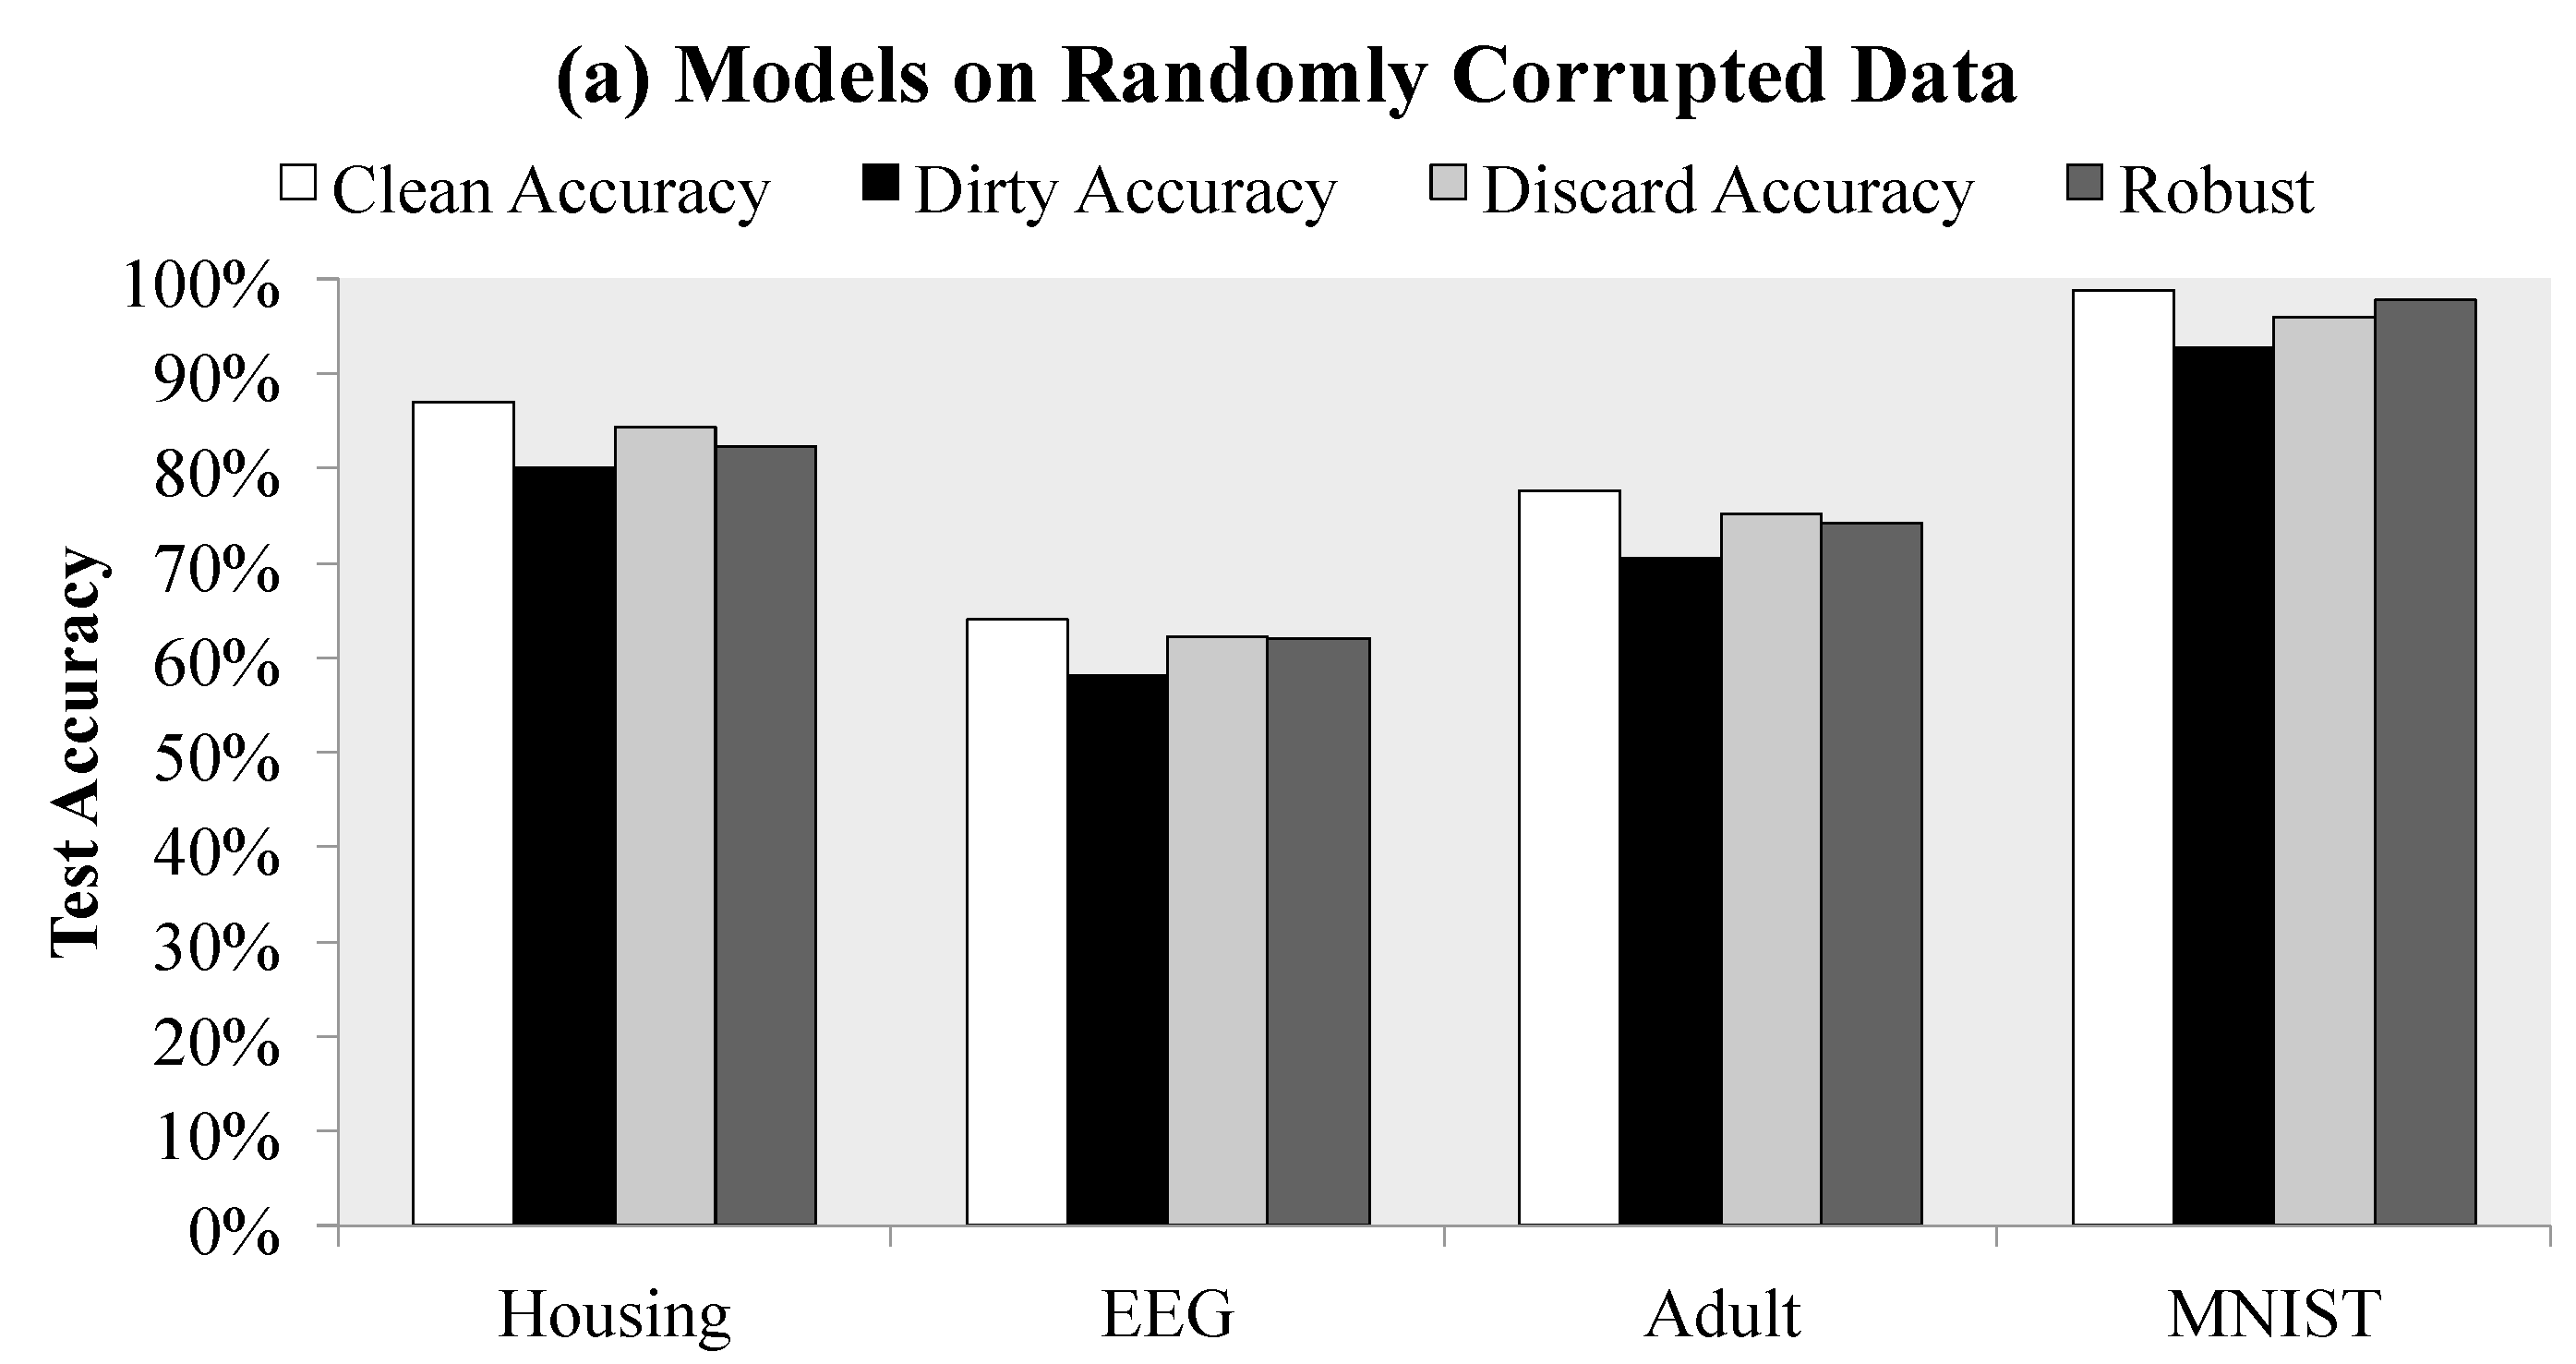
\includegraphics[width=0.8\columnwidth]{exp/exp2.pdf}
 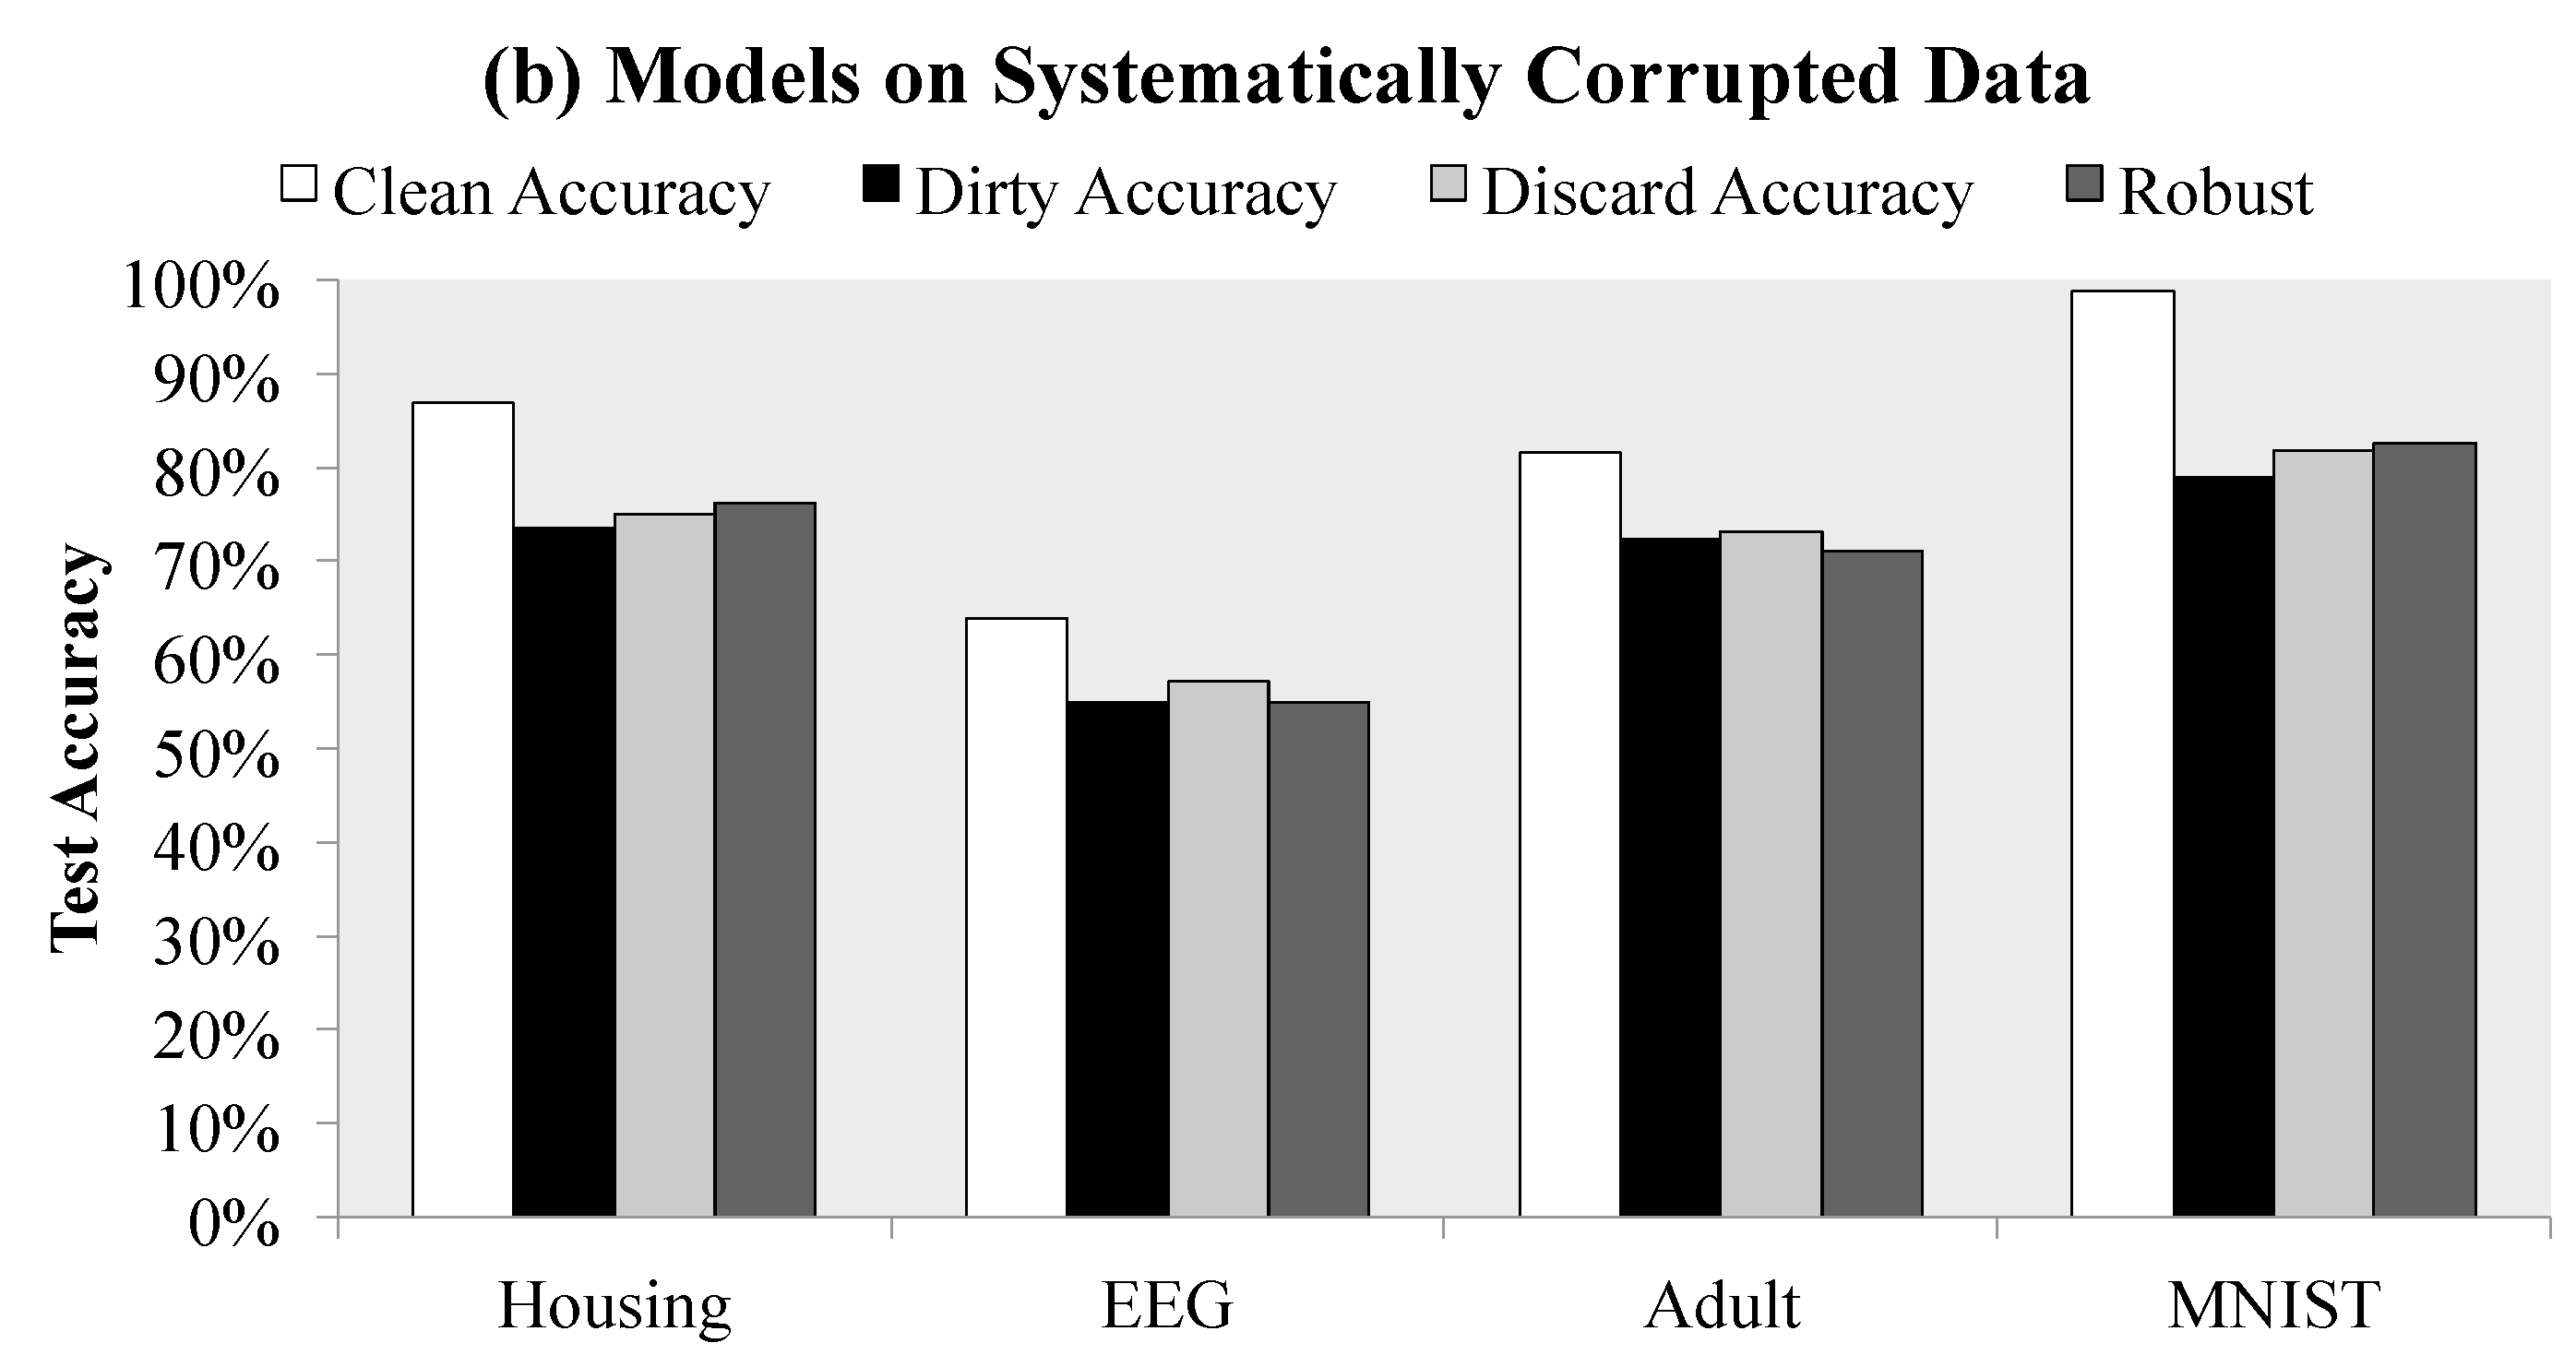
\includegraphics[width=0.8\columnwidth]{exp/exp1.pdf}
 \caption{Robust techniques work best when corrupted data are random and look atypical. Data cleaning can provide reliable performance in both the systematically corrupted setting and randomly corrupted setting.\label{sys-rand}}
\end{figure}

In Figure \ref{sys-rand}, we present the results of this experiment.
As we argued in this paper, the robust method performs well on the random high-magnitude outliers, however, falters on the systematic corruption.
Interestingly enough, in the random setting, discarding dirty data also performs well.
However, when errors are systematic data cleaning is the most reliable option across datasets.
In the MNIST dataset, we see a particularly significant effect of systematic corruption
where the test accuracy drops from nearly 98\% to 78\%.
Multiclass classification is particularly sensitive to systematic corruption when the corruptions can make classes ambiguous (e.g. reconizing a ``4" and a ``9").
The problem is that a priori, we do not know if data error is random or systematic.
While data cleaning requires more effort, it provides benefits in both settings.

\subsection{Experiment 2. Prioritization}
The next set of experiments evaluate different approaches to cleaning a sample of data.
In this set of experiments, we use the random errors generated above.

\subsubsection{2a. Alternative Algorithms}
In our first prioritization experiment, we evaluate the samples-to-error tradeoff between three alternative algorithms:

\noindent\textbf{SampleClean (SC): } In SampleClean, we do not use a gradient update and instead take a sample of data and train the model to completion on the sample.

\noindent\textbf{Active Learning (AL): } In Active Learning, we do not consider the effect of ``data cleaning" and prioritze points by their dirty gradient value. We do, however, do this iteratively and update the model.

\noindent\textbf{ActiveClean Oracle (AC+O): } In ActiveClean Oracle, we importance sample points by their clean gradient. This represents the theoretical best that our algorithm could hope to achieve given perfect error estimation.

In Figure \ref{prio-perf}, we present our results on Housing, Adult, and EEG. 
We find that \sys gives its largest benefits for small sample sizes (up-to 12x).
\sys makes significant progress because of its intelligent initialization, iterative updates, and partitioning.
For example, the EEG dataset is the hardest classification task.
SampleClean has difficulty on this dataset since it takes a uniform sample of data (only 5\% of which are corrupted on average) and tries to train a model using only this data.
\sys and Active Learning leverage the initialization from the dirty data to get an improved result. 
However, \sys's impact estimates and error partitioning allow us to beat Active Learning on all three of the datasets.

\begin{figure*}[t]
\centering
 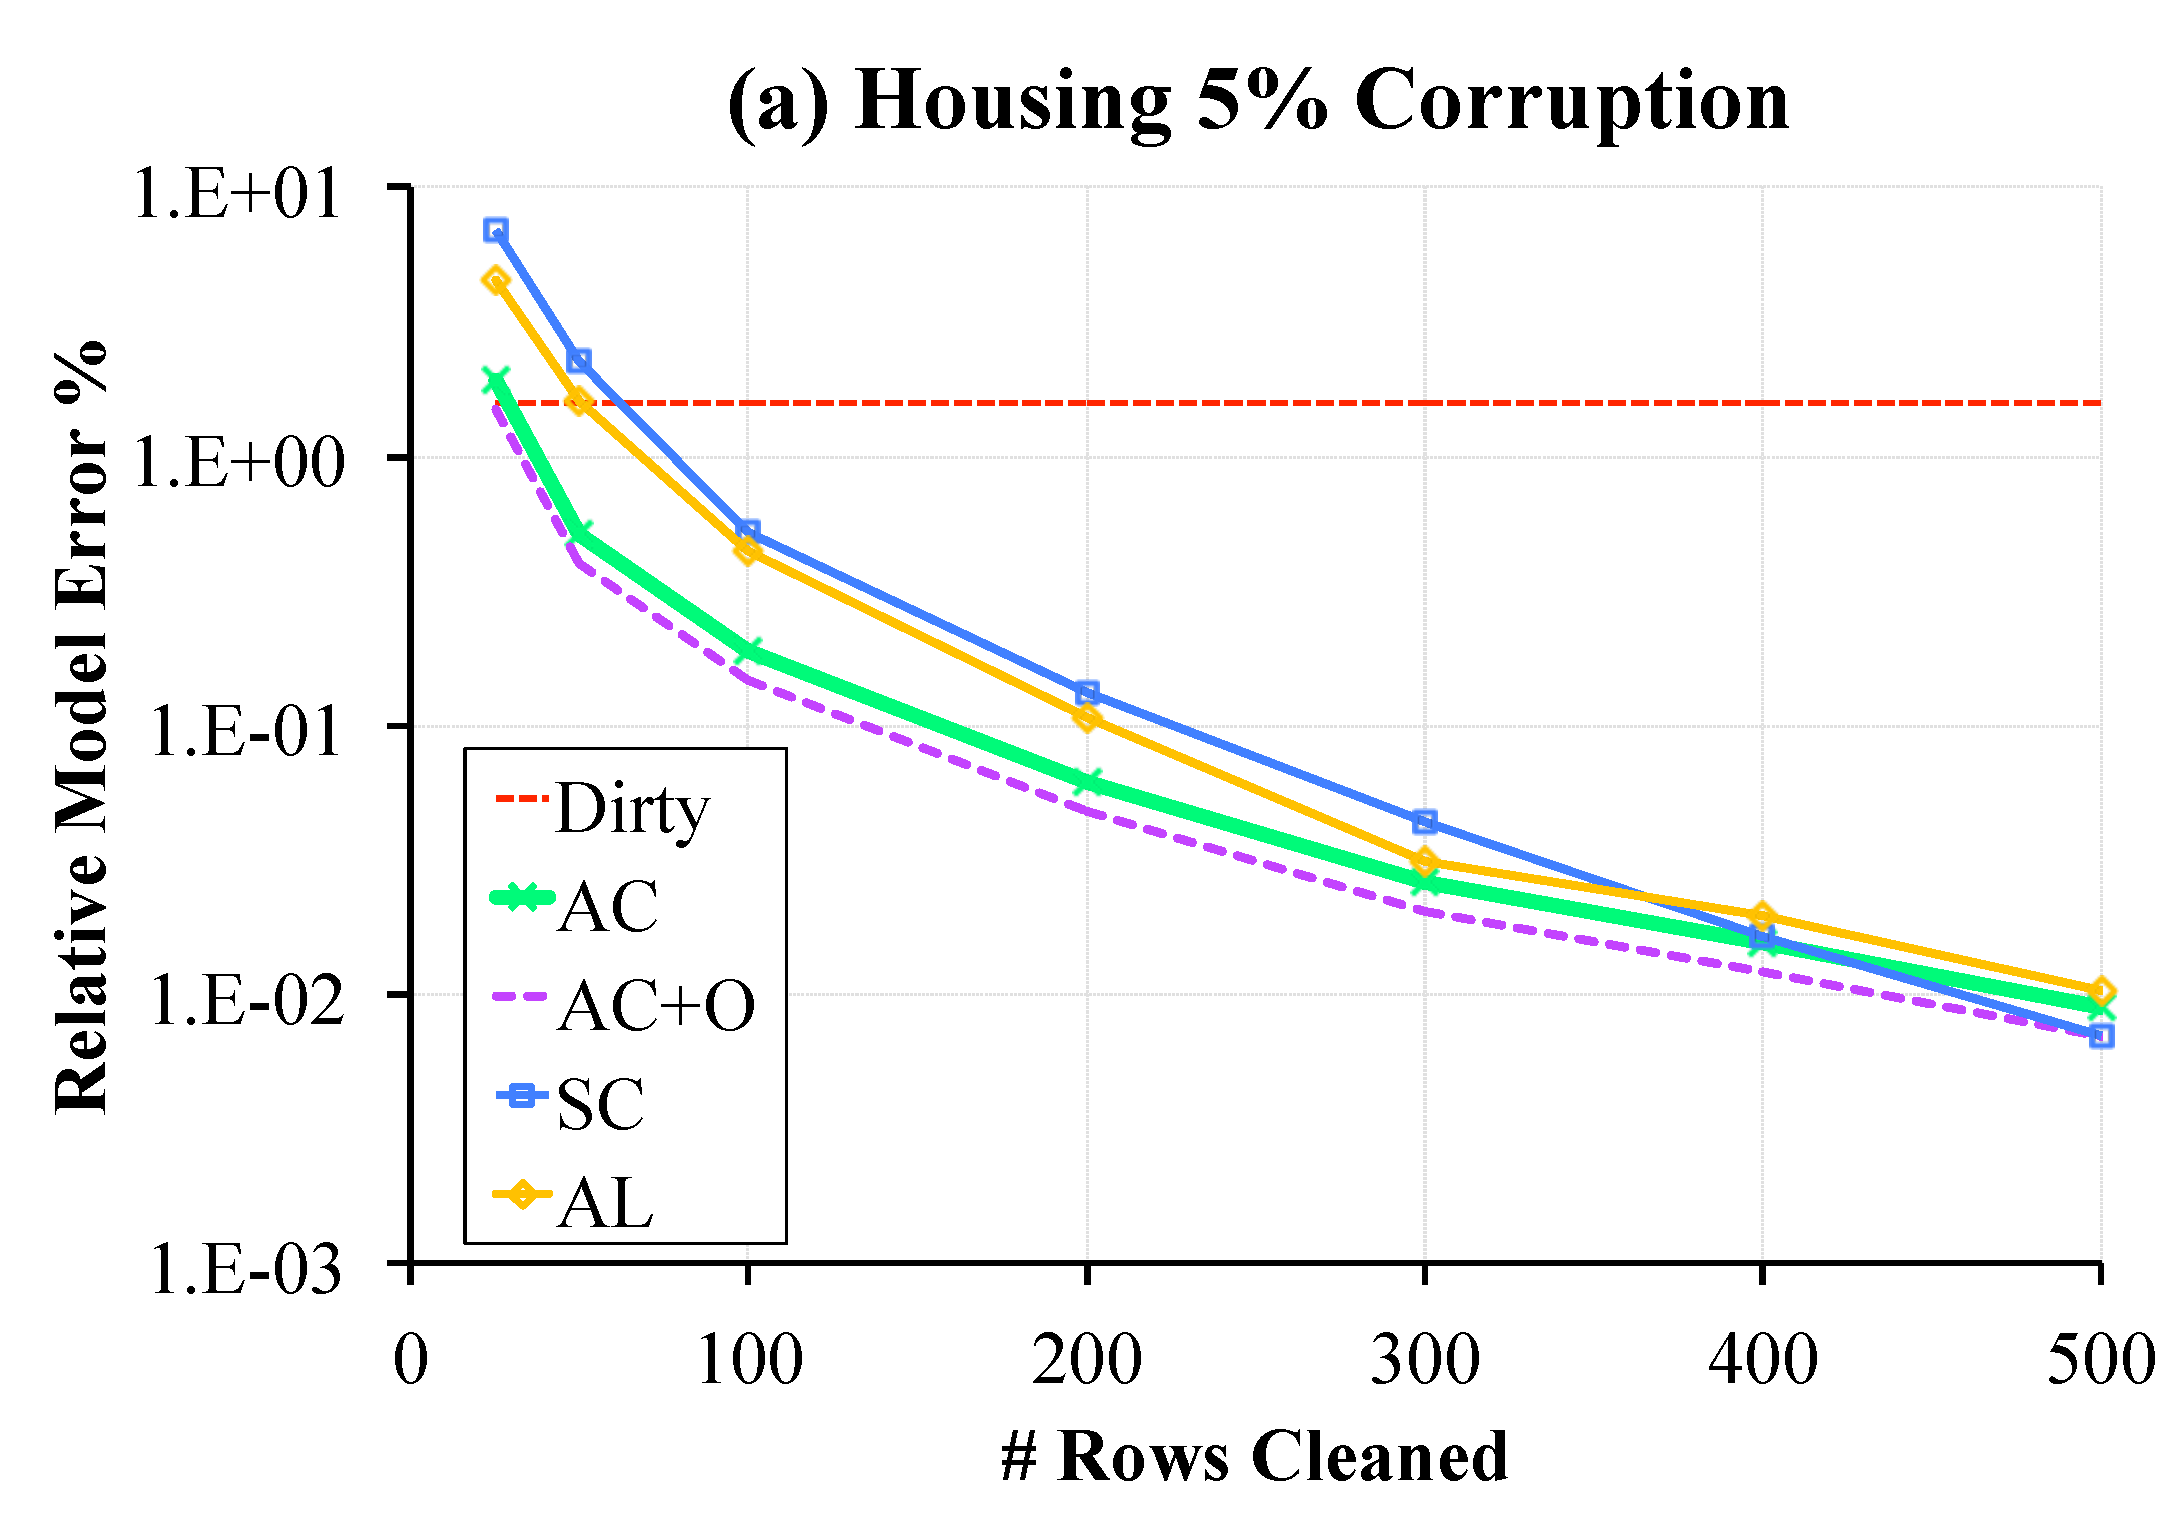
\includegraphics[scale=0.15]{exp/exp3a.pdf}
 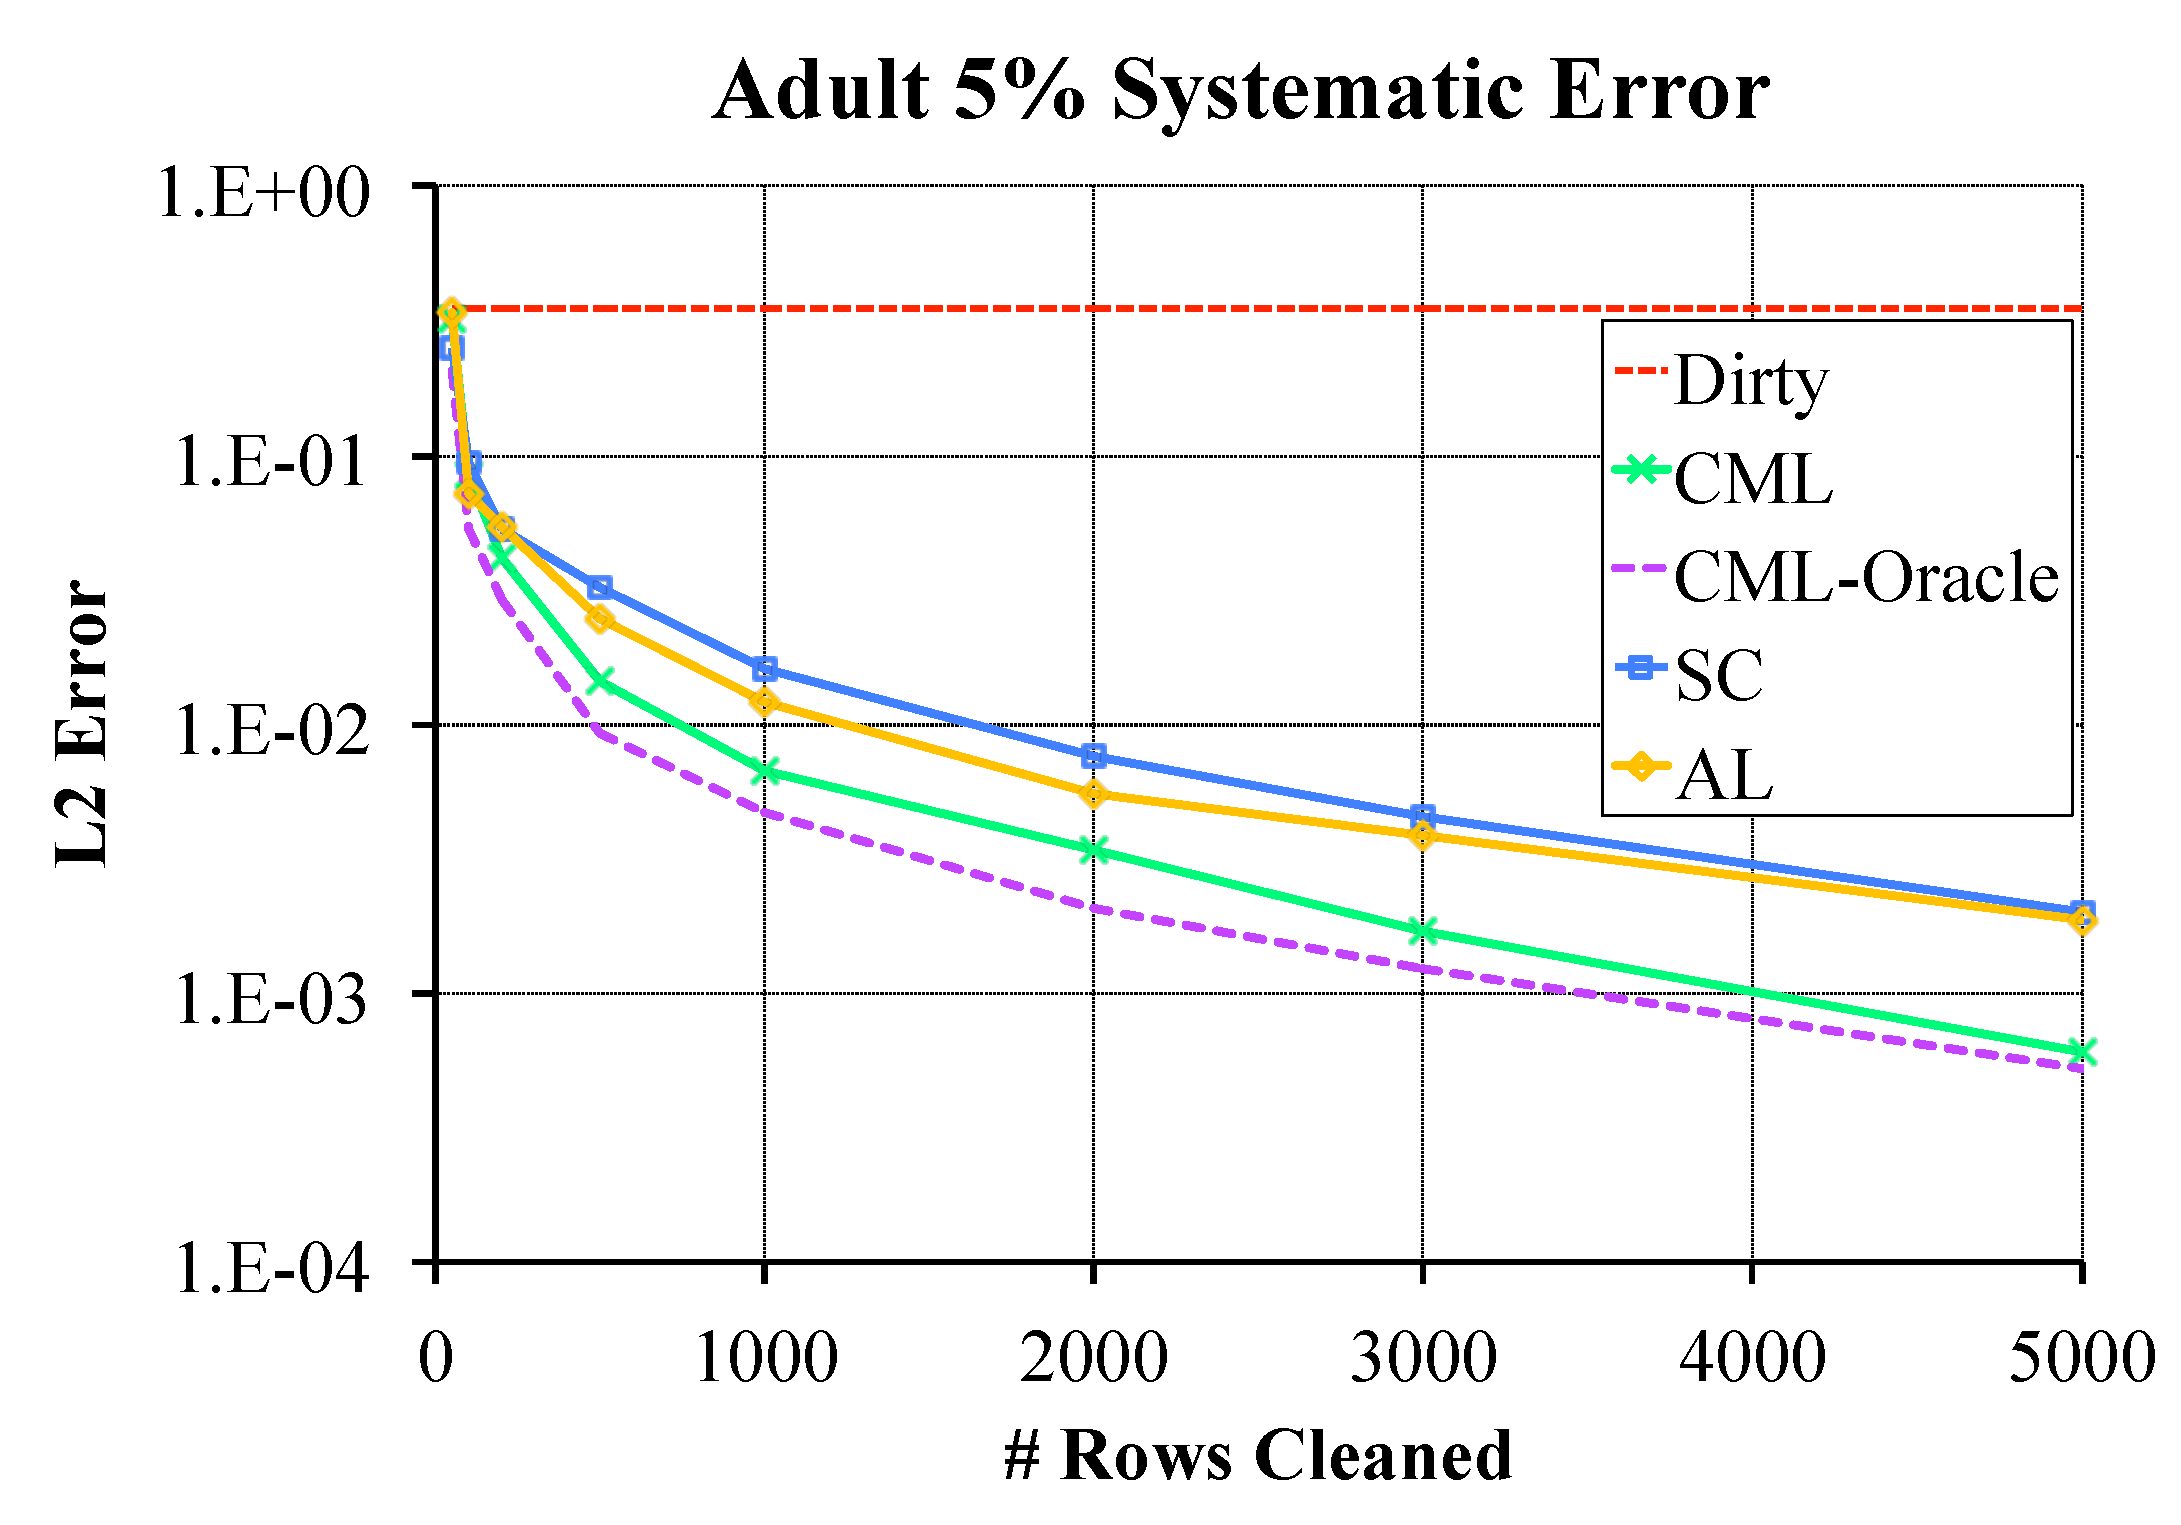
\includegraphics[scale=0.15]{exp/exp3b.pdf}
  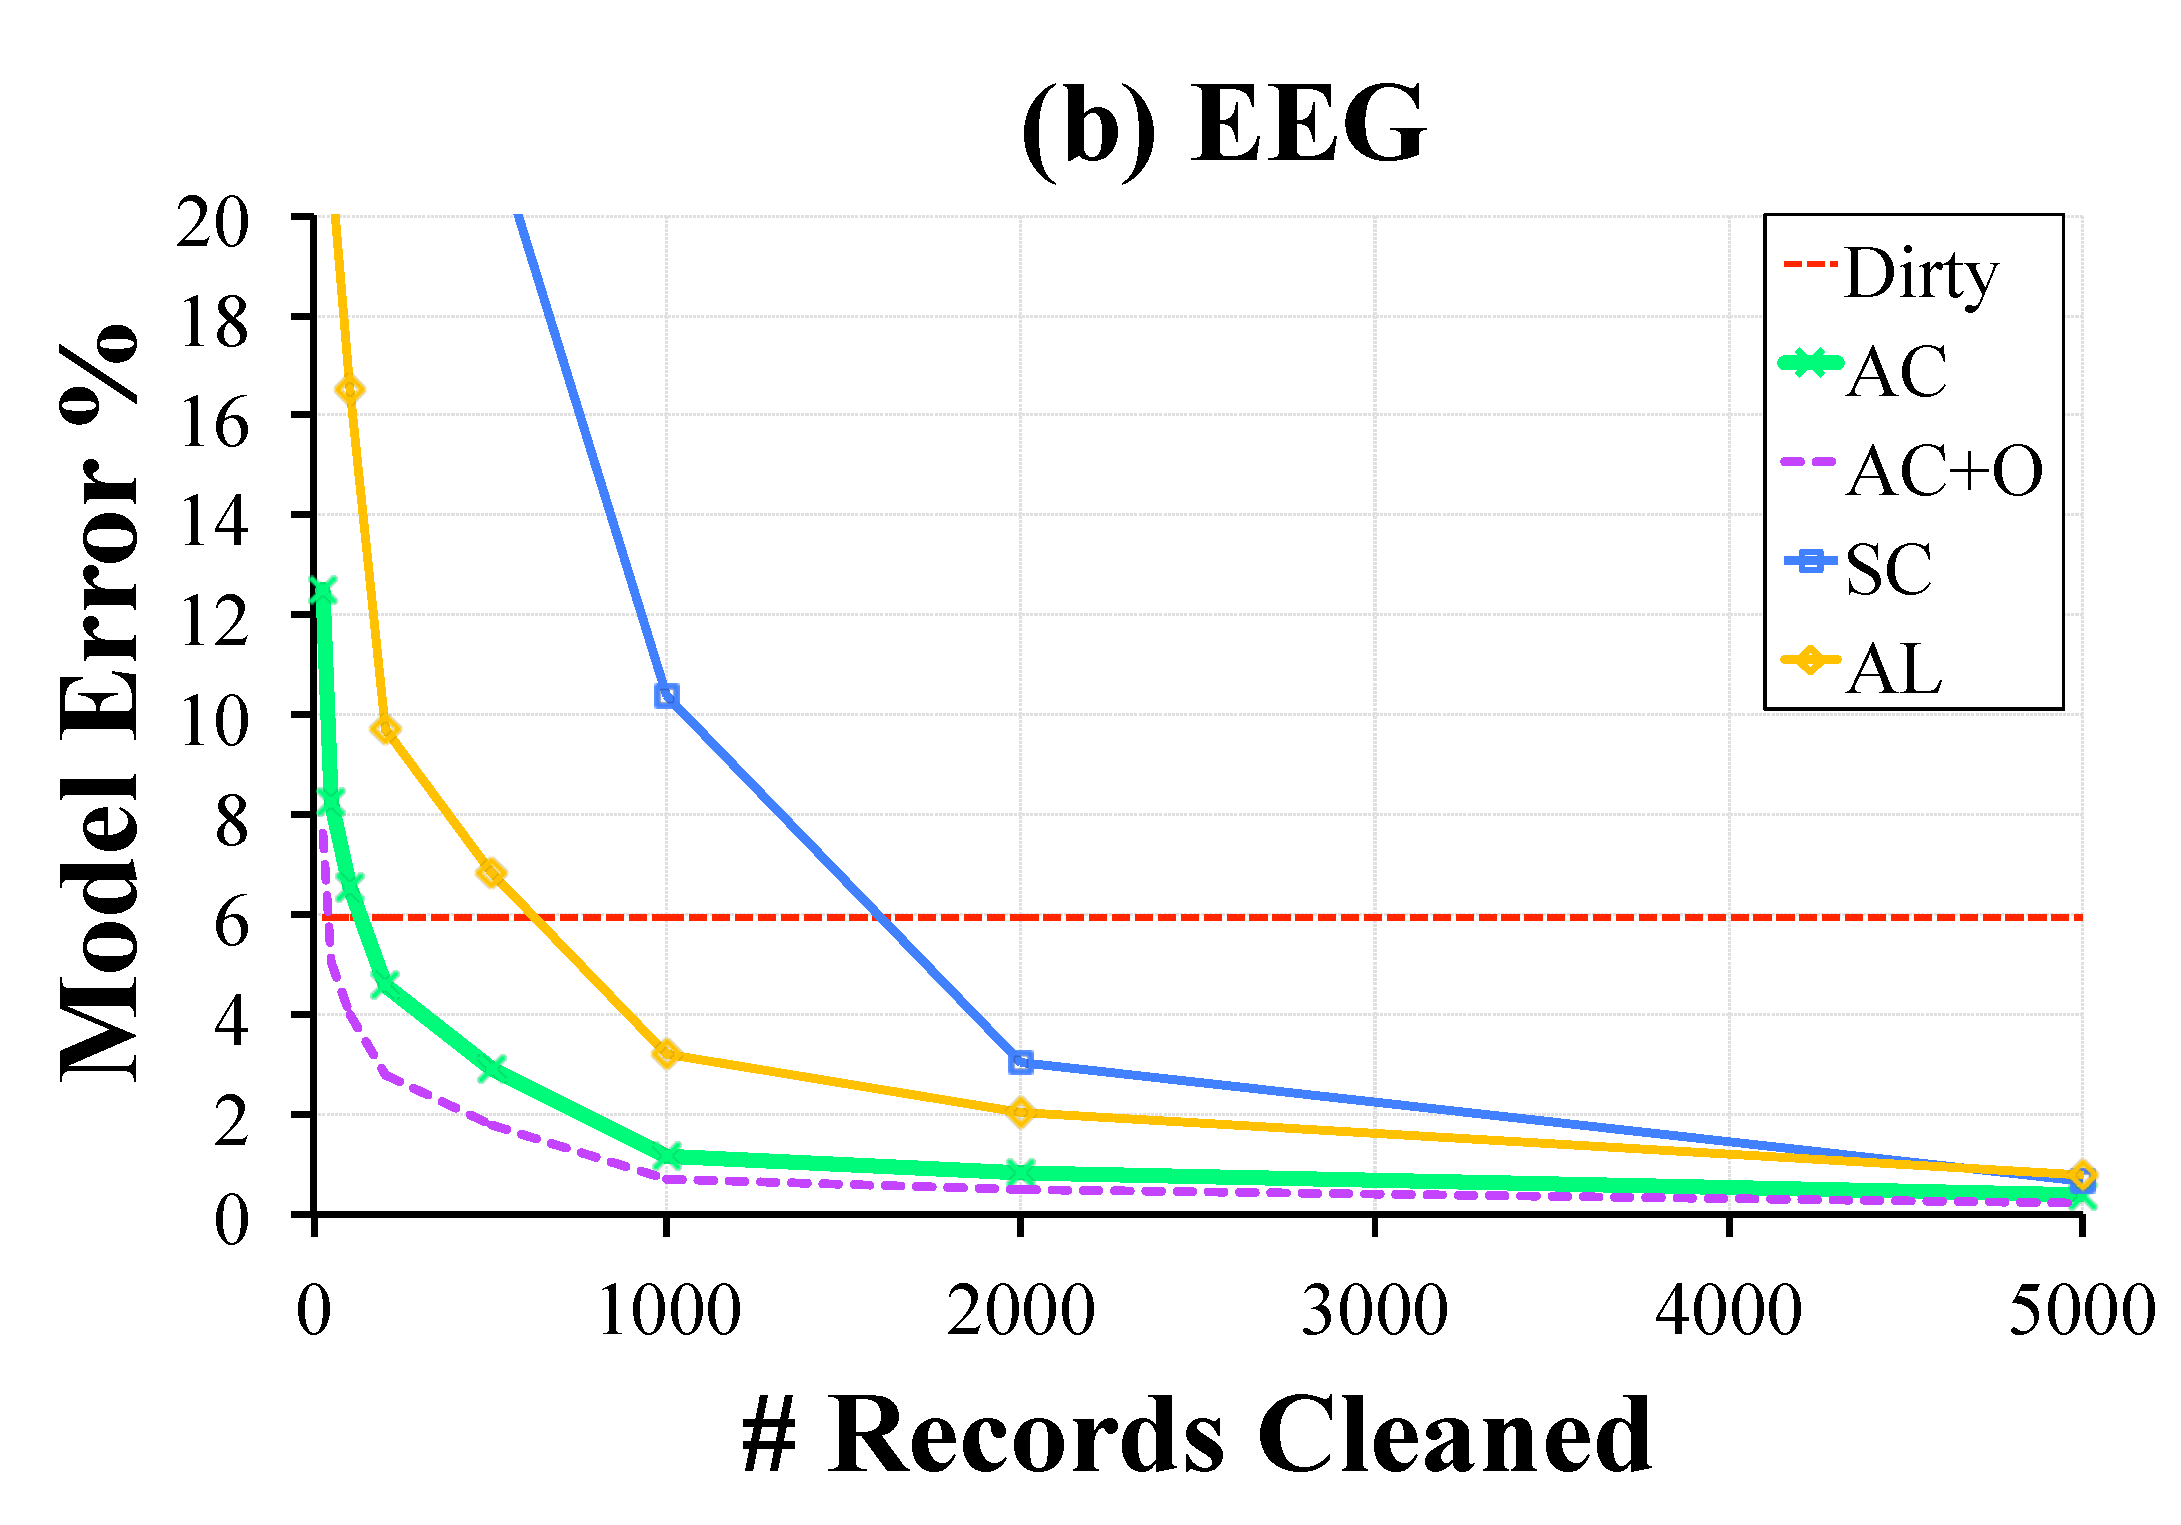
\includegraphics[scale=0.15]{exp/exp3c.pdf}
 \caption{\sys converges with a smaller sample size to the true result in comparison to Active Learning and SampleClean. \label{prio-perf}}
\end{figure*}

\subsubsection{2b. Source of Improvements}
Throughout the paper, we proposed numerous optimizations.
Now, we try to understand the source of our improvements w.r.t Active Learning and SampleClean.
We pick a single point on the curves shown in Figure \ref{prio-perf} that corresponds to 10\% of the data cleaned (55 for Housing, 4555 for Adult, 150 for EEG) and compare the performance of \sys with and without various optimizations.
We denote \sys without partitioning as (AC-P) and \sys without partitioning and importance sampling as (AC-P-I).
In Figure \ref{opts}, we plot the relative error of the alternatives w.r.t to the optimized version of \sys.
Partitioning significantly improves our results in all of the datasets, and accounts for a substantial part of the improvements over Active Learning.
However, when we remove partitioning we still see some improvements since our importance sampling relies on error impact estimates that judge how valuable a point is to the clean model rather than the dirty model in Active Learning.
Not surprisingly, when we remove both these optimizations, \sys is comparable or slightly worse than Active Learning.

\begin{figure}[ht!]
\centering
 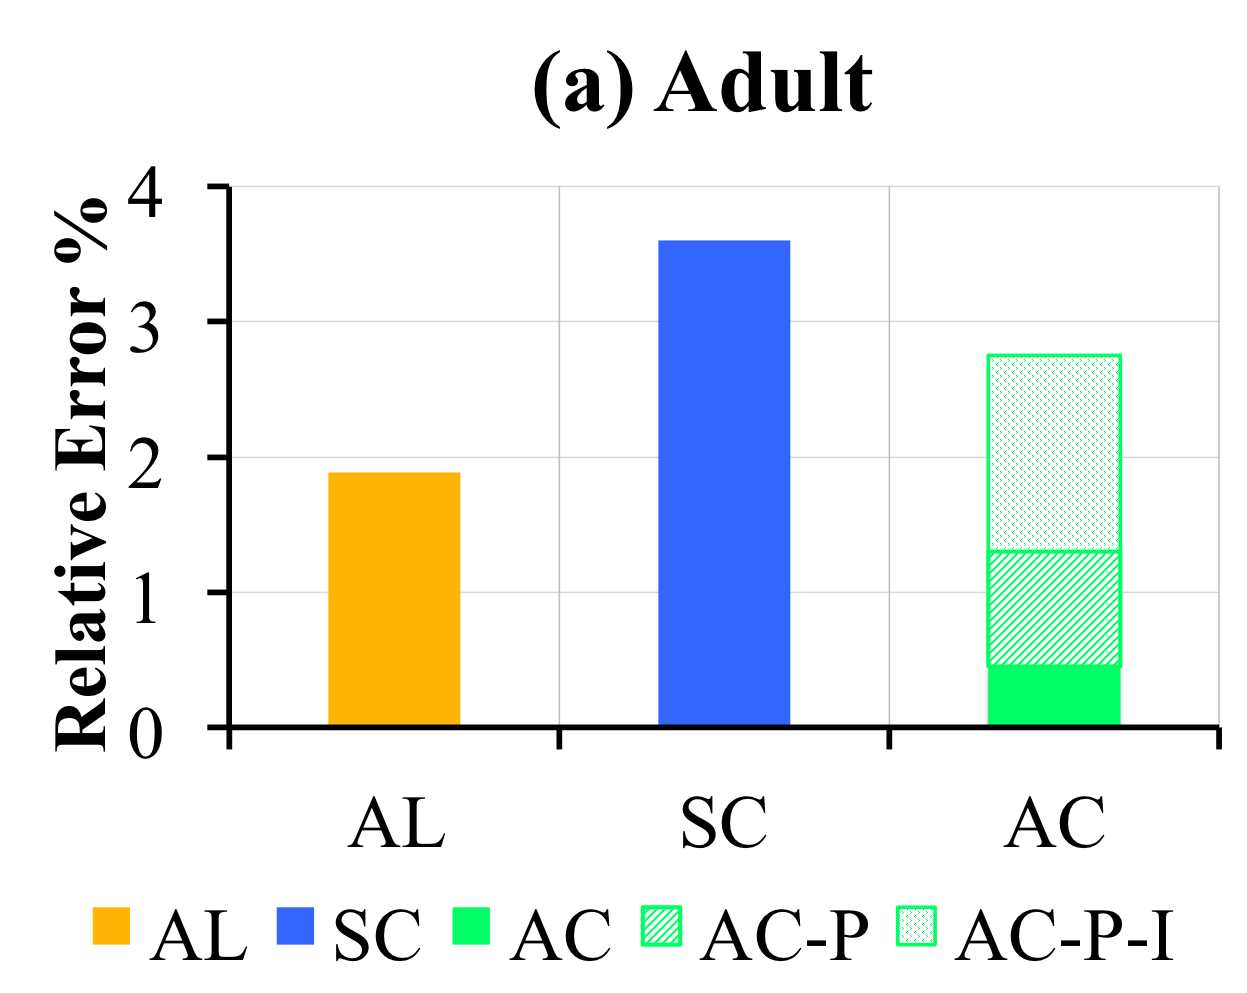
\includegraphics[width=\columnwidth]{exp/exp8.png}
 \caption{We clean 10\% of the data with the alternative algorithms and also include variants of \sys with optimization removed. We plot the relative error w.r.t the optimized \sys. Both partitioning and importance sampling lead to significant reductions in error. \label{opts}}
\end{figure}

We evalue Active Learning and \sys to better understand this relationship.
In Figure \ref{albias}, we vary the biasing effect of our random corruptions.
That is, we start with zero mean noise and increase the mean value and variance of the noise.
Since Active Learning uses the gradient, if there is zero mean noise, in expectation, the dirty data and clean data are the same.
However, as the bias increases, the fact that Active Learning prioritizes w.r.t to the dirty data matters more and becomes increasingly erroneous w.r.t to \sys.

\begin{figure}[ht!]
\centering
 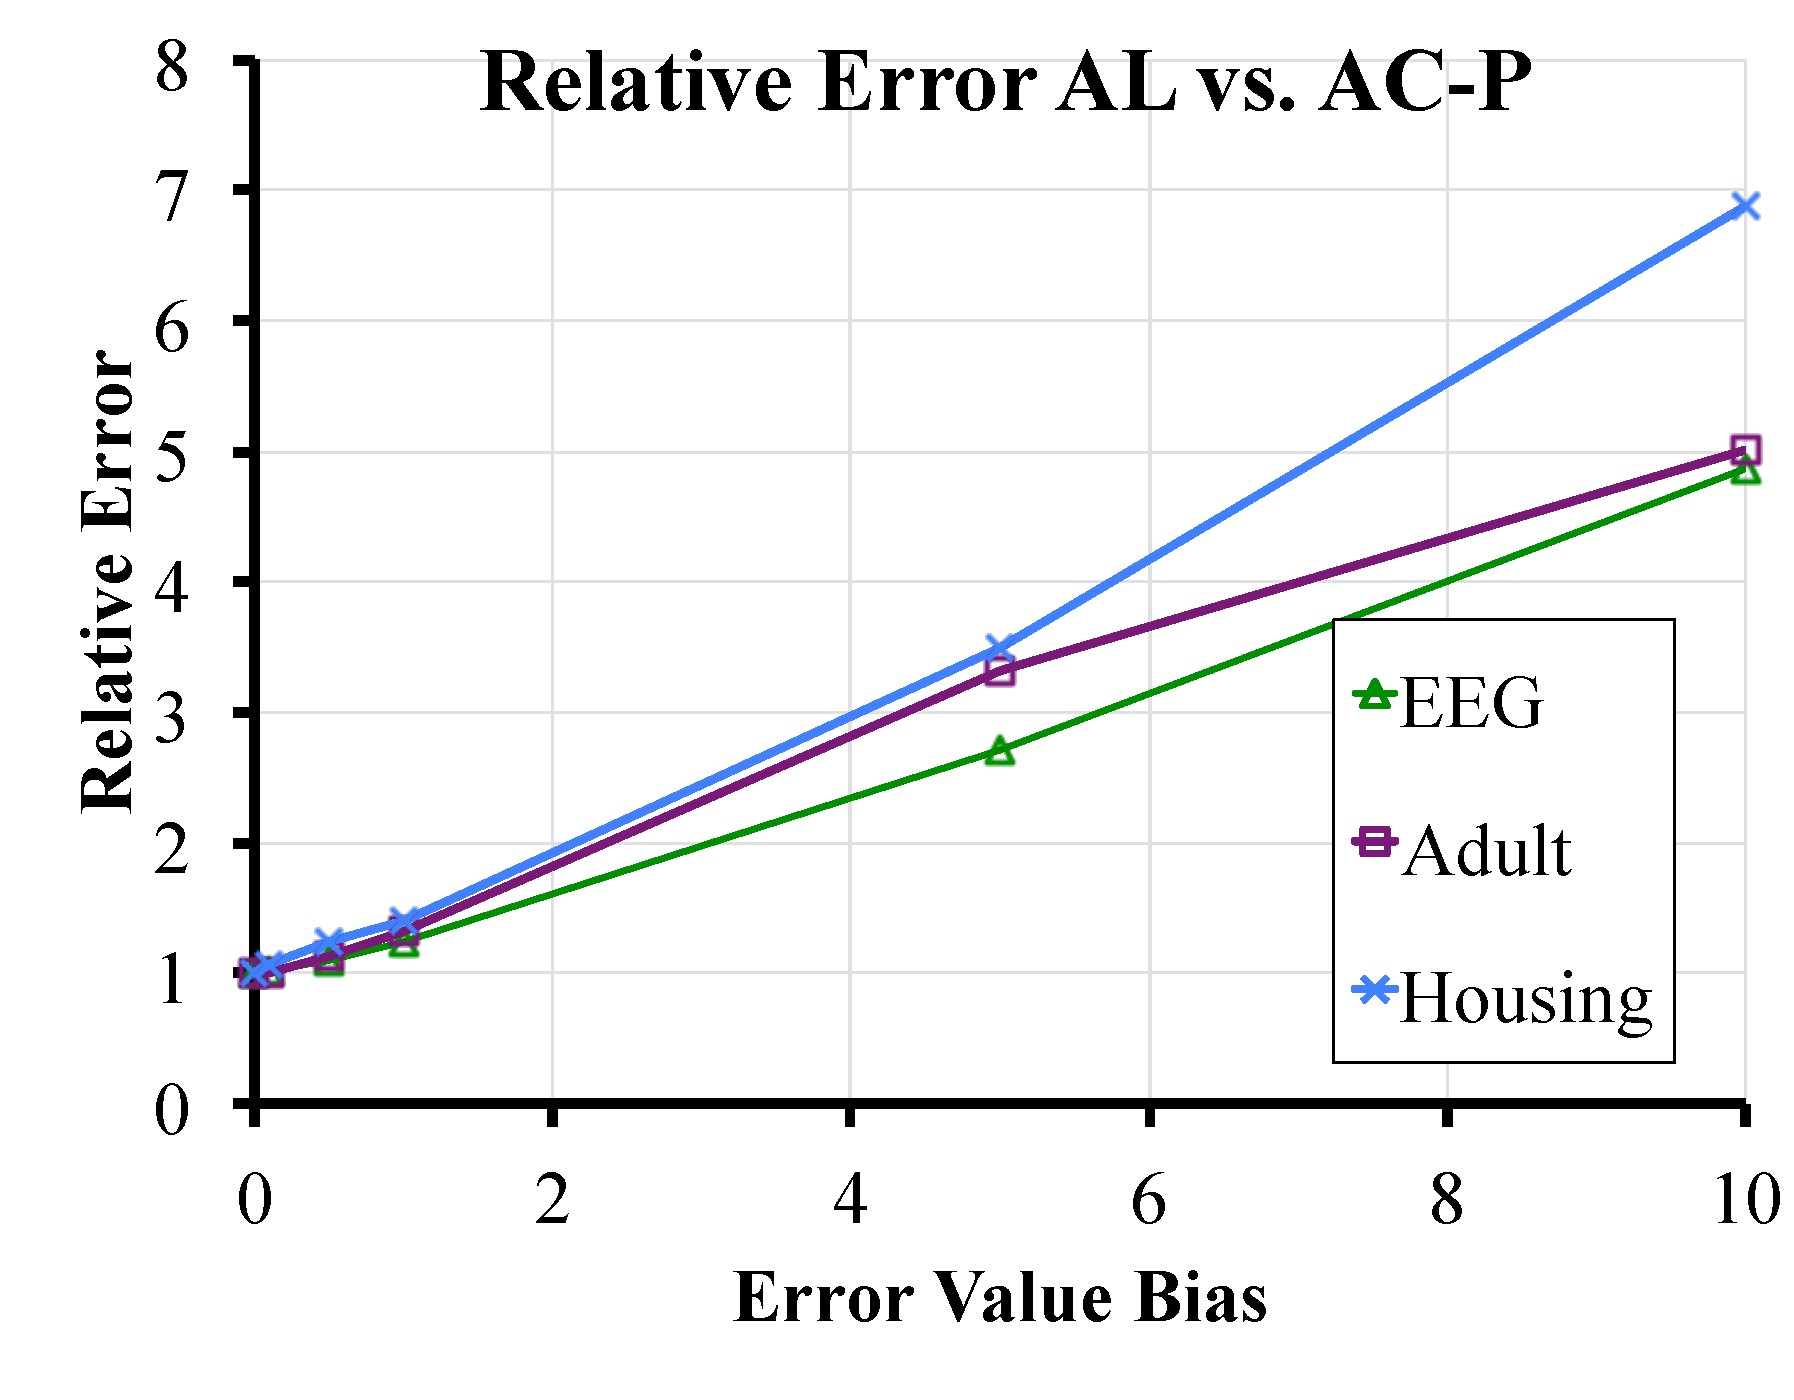
\includegraphics[width=0.6\columnwidth]{exp/exp10.pdf}
 \caption{As we increase the biasing nature of the corruption, Active Learning is increasingly erroneous w.r.t \sys. \label{albias}}
\end{figure}

\subsubsection{2c. Error Dependence}
Both Active Learning and \sys outperform SampleClean in our experiments.
In our next experiment, we try to understand how much of this performance 
is due to the initialization (i.e., SampleClean trains a model from ``scratch").
We vary the rate of random error, thus making the initialization more and more arbitrary, 
and measure the relative performance between SampleClean and \sys.
Since SampleClean only acts on a clean sample of data, it is robust to data error.
So at some point, the errors in the data are so significant that training a model on a small but clean sample of data is more efficient than iteratively updating the dirty model.

In Figure \ref{bias}, we present the results from this experiment.
We corrupt entries from the data matrix of the Adult dataset at random (probability on plotted on the x-axis).
Then, we measure the number of records we need to clean before we have a relative error of 0.1\%.
We find that at about 30\% corruption rate, SampleClean is more accurate than \sys.
Since the Adult dataset has 12 features, a 30\% corruption rate corresponds to each example with 3.6 features incorrect on average.
We optimized \sys for sparse and relatively small errors but it still shows reasonable performance even in this highly erroneous setting. 
At higher corruption rates, \sys requires more than one epoch to converge to an accurate answer which requires cleaning almost all of the data.

\begin{figure}[ht!]
\centering
 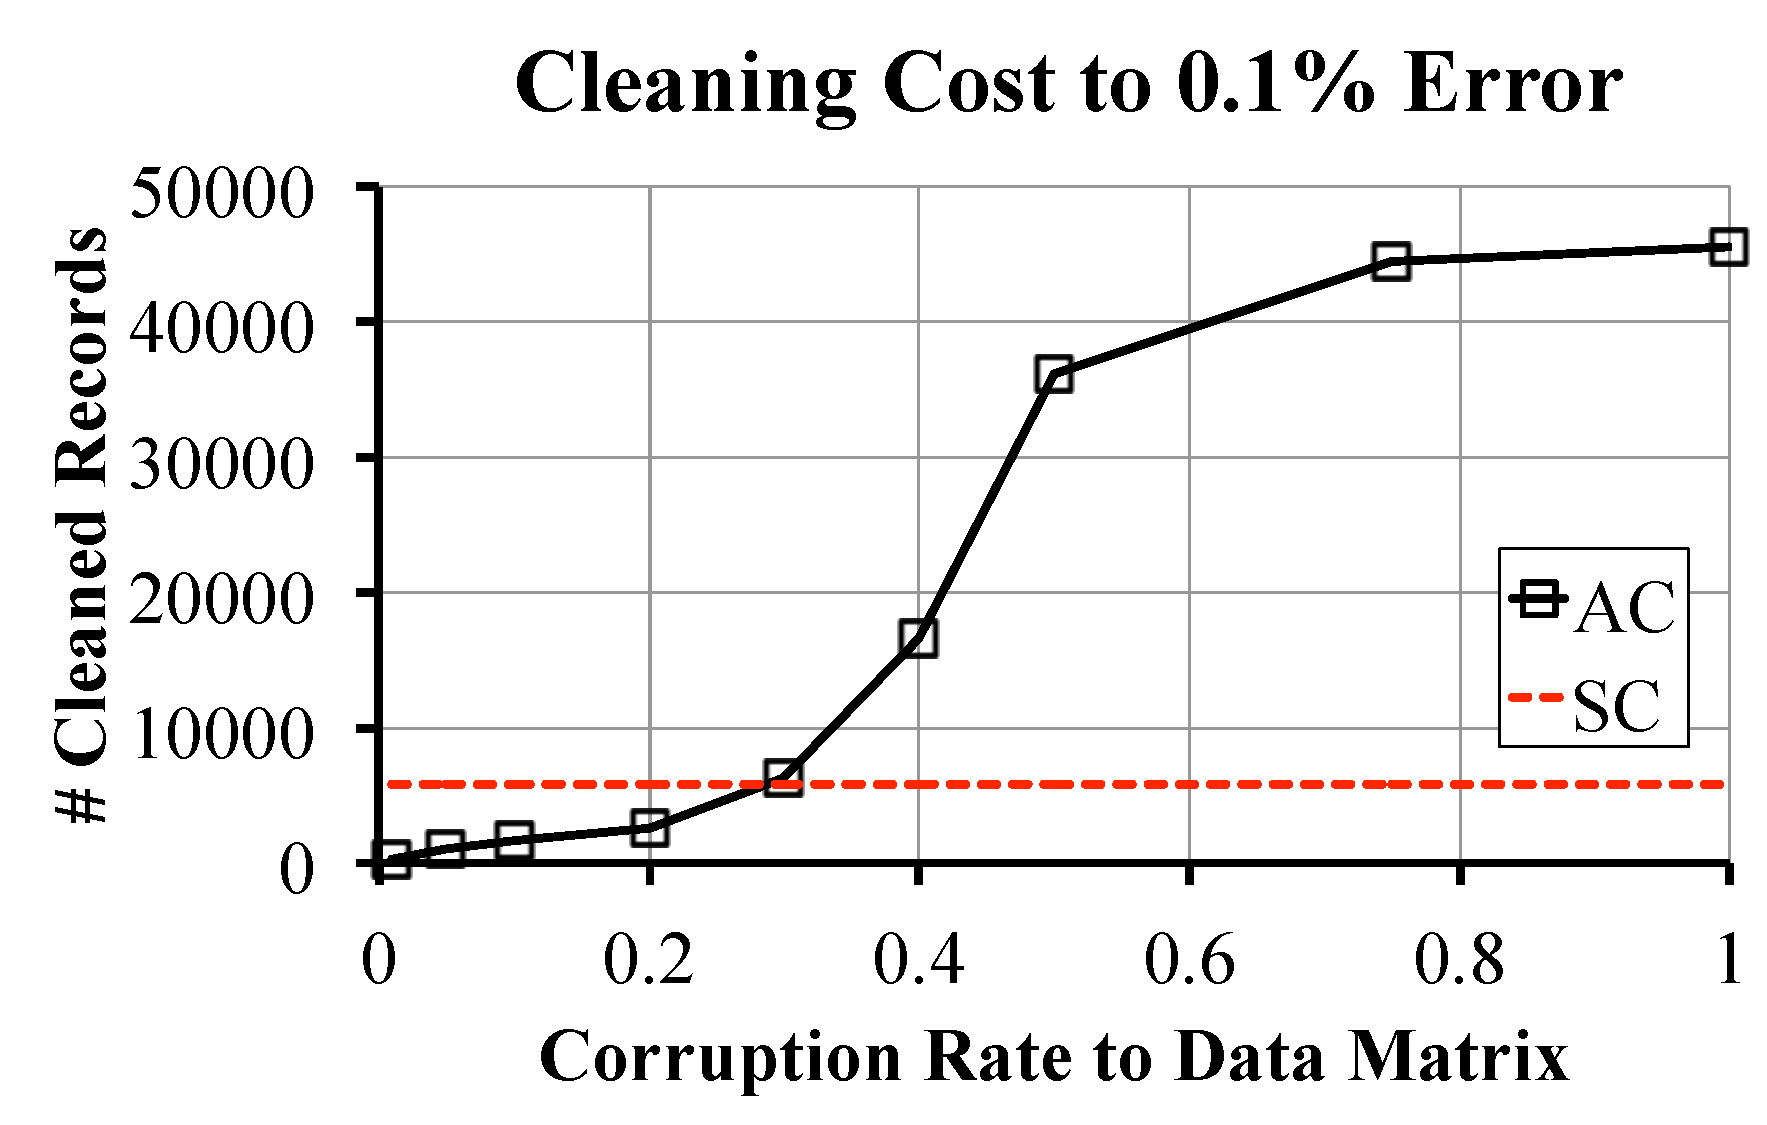
\includegraphics[width=0.6\columnwidth]{exp/exp9.pdf}
 \caption{We corrupt an increasing number of entries in the data matrix. At about 30\% corrupted, \sys is no longer more efficient than SampleClean. \label{bias}}
\end{figure}

\subsubsection{2d. Testing Accuracy}
In the previous experiments, we studied the relative model error which measures the training loss. 
However, to an end user the metric that matters is test accuracy.
In the next experiment, we try to understand how reductions in model error correlate to improvements in test error.
In Figure \ref{prio-tperf}, we present the results for the three datasets: Adult, Housing, and EEG.
We find that in two of the datasets, Housing and Adult, \sys converges to clean test accuracy faster than the alternatives.

However, there is a curious negative result with the EEG dataset that we would like to highlight. 
We find that even though \sys has significantly lower model error (Figure \ref{prio-perf}), this does not correspond to as significant of an increase in test accuracy.
We speculate this is due to the inherrent hardness of the EEG classification problem.
\sys may encourage overfitting at intermediate results for hard classification tasks.
The solution to this problem may be to add additional regularization, thus actually changing the optimization problem.
We hope to explore this problem in further detail in future work.

\begin{figure*}[t]
\centering
 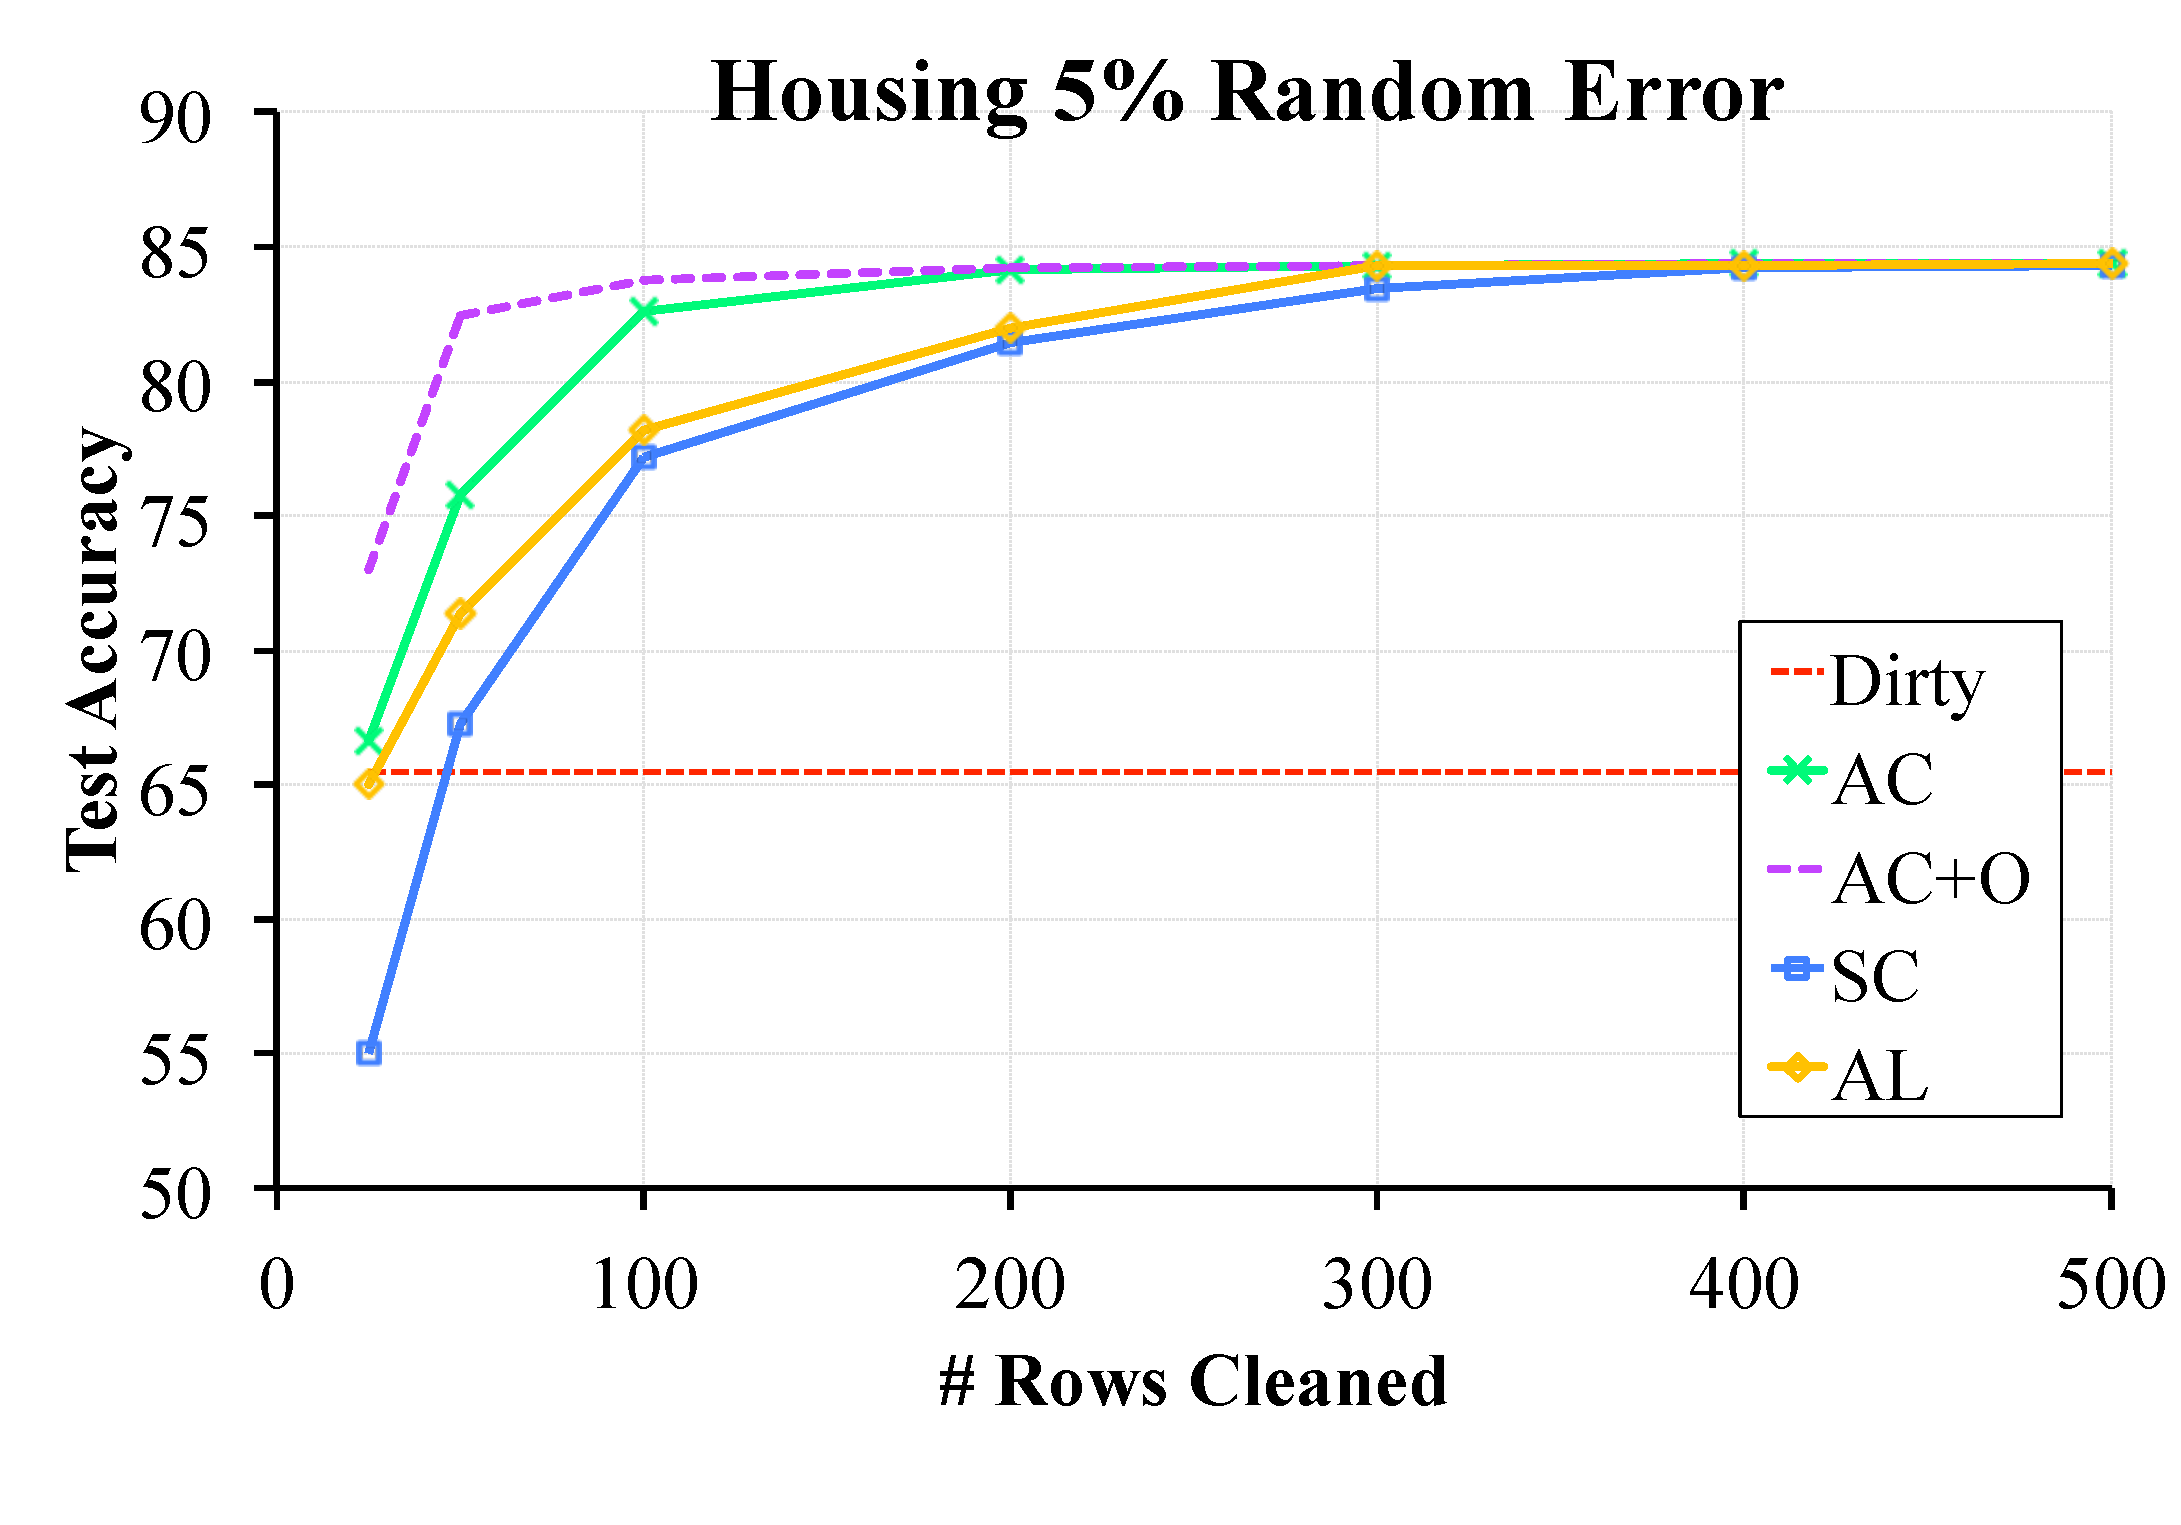
\includegraphics[scale=0.15]{exp/exp3aa.pdf}
 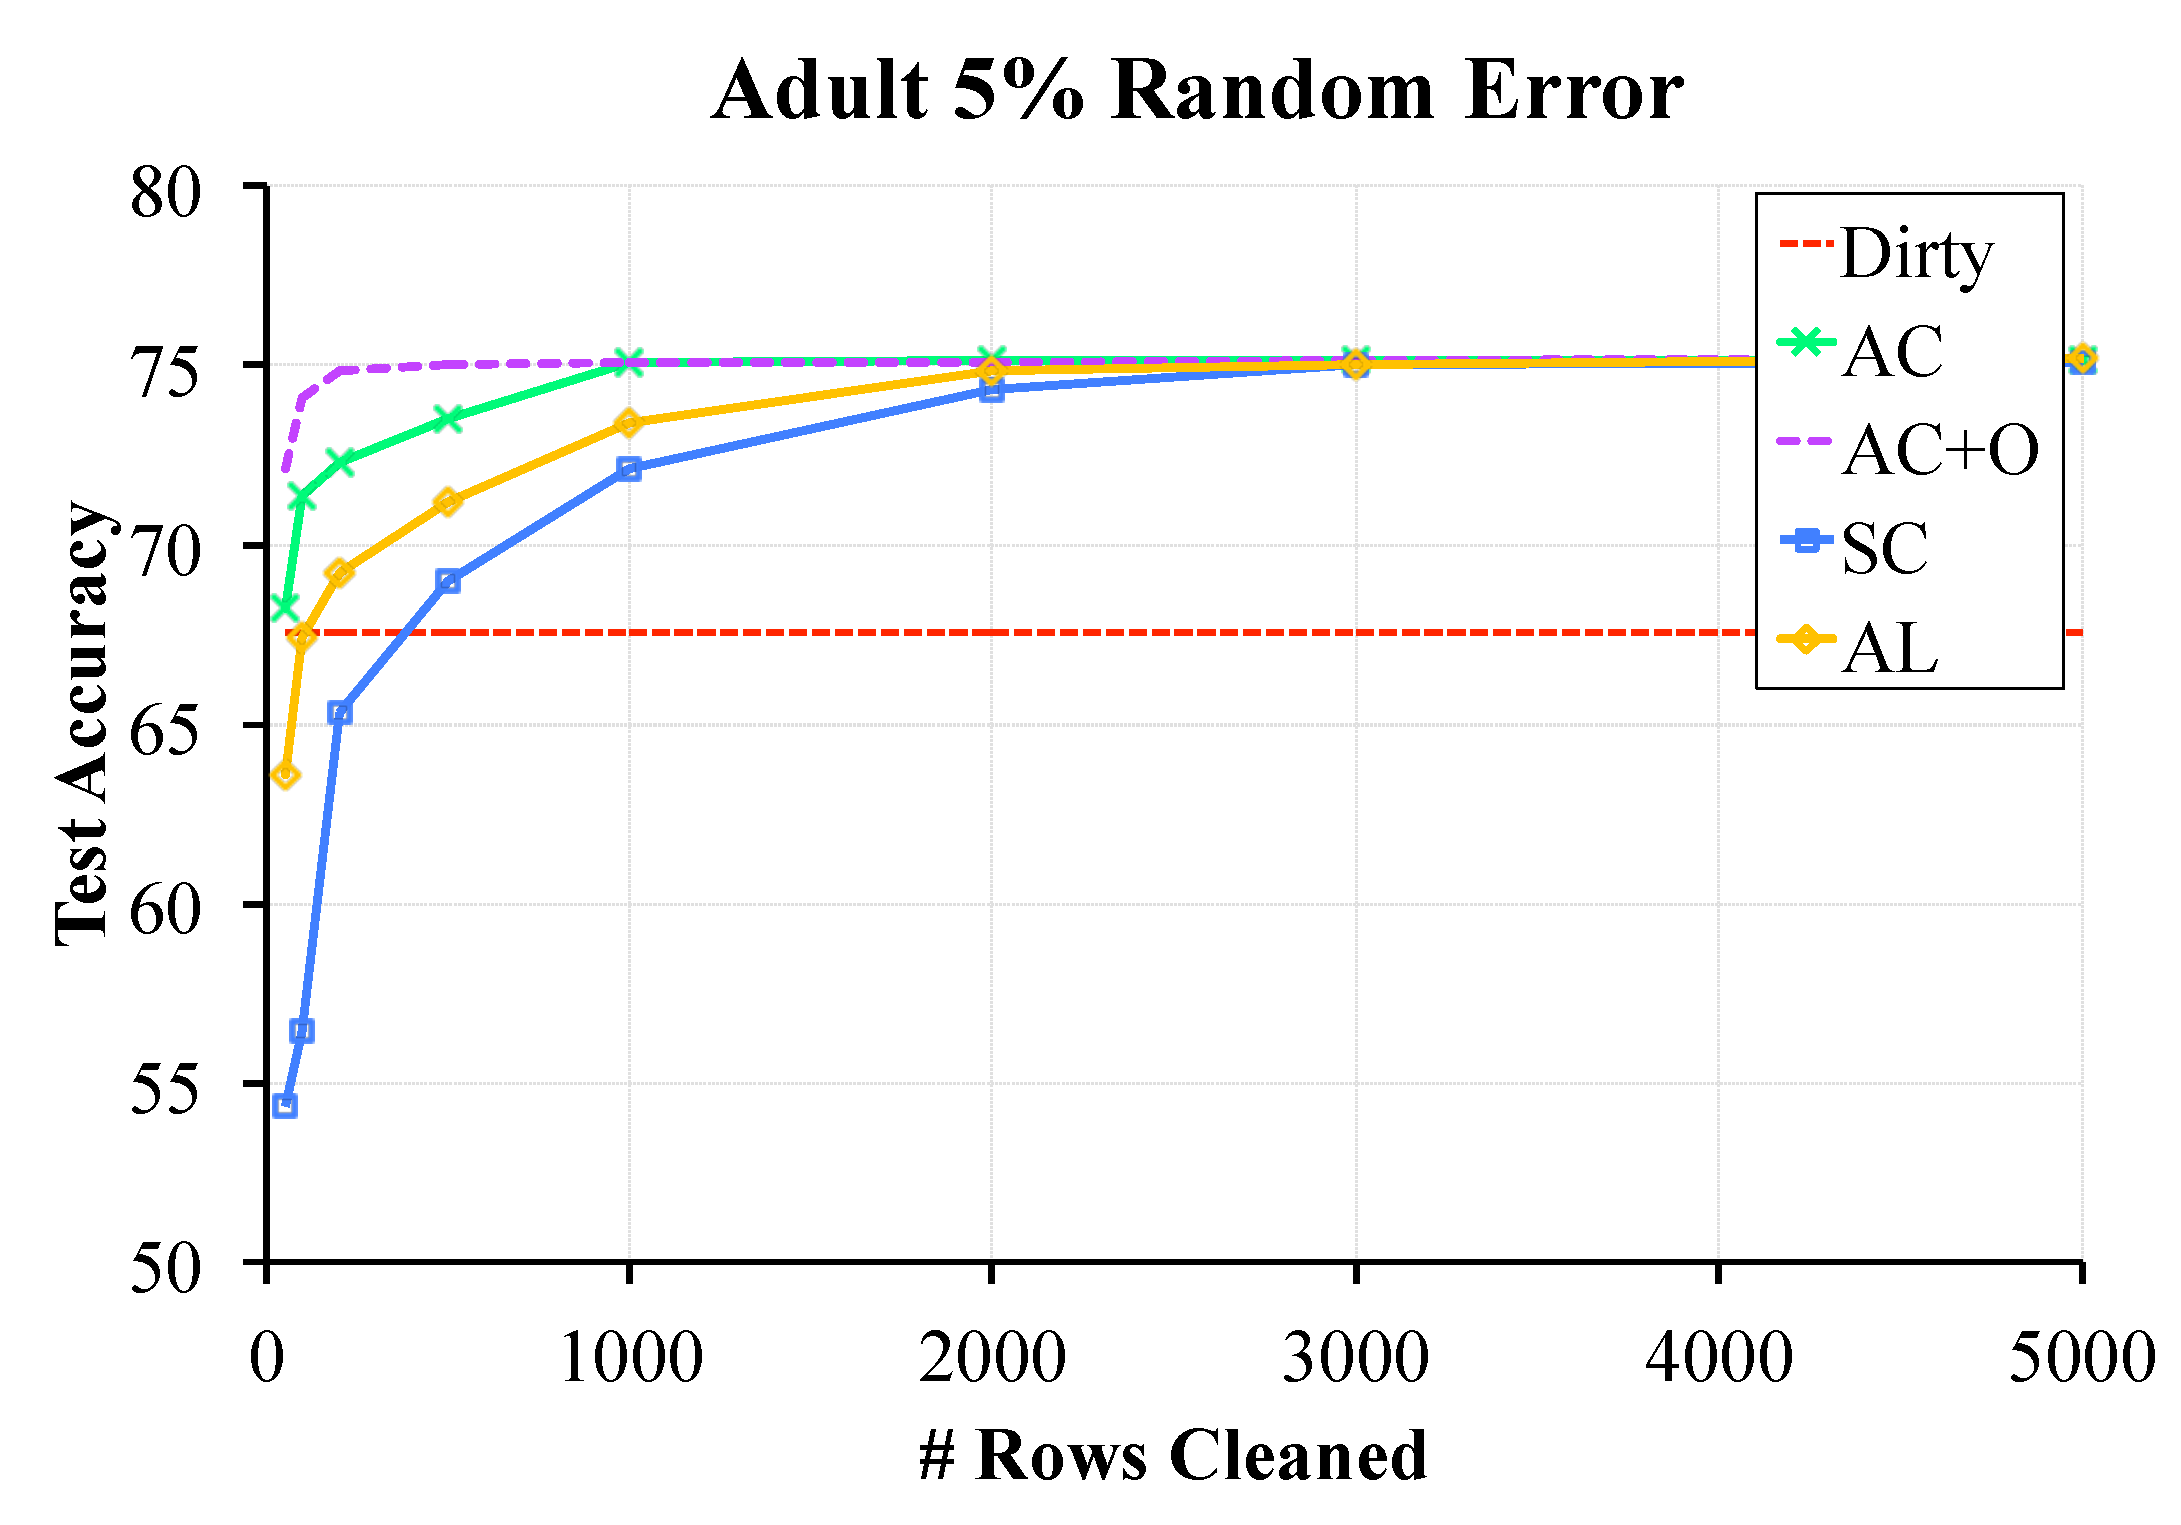
\includegraphics[scale=0.15]{exp/exp3bb.pdf}
  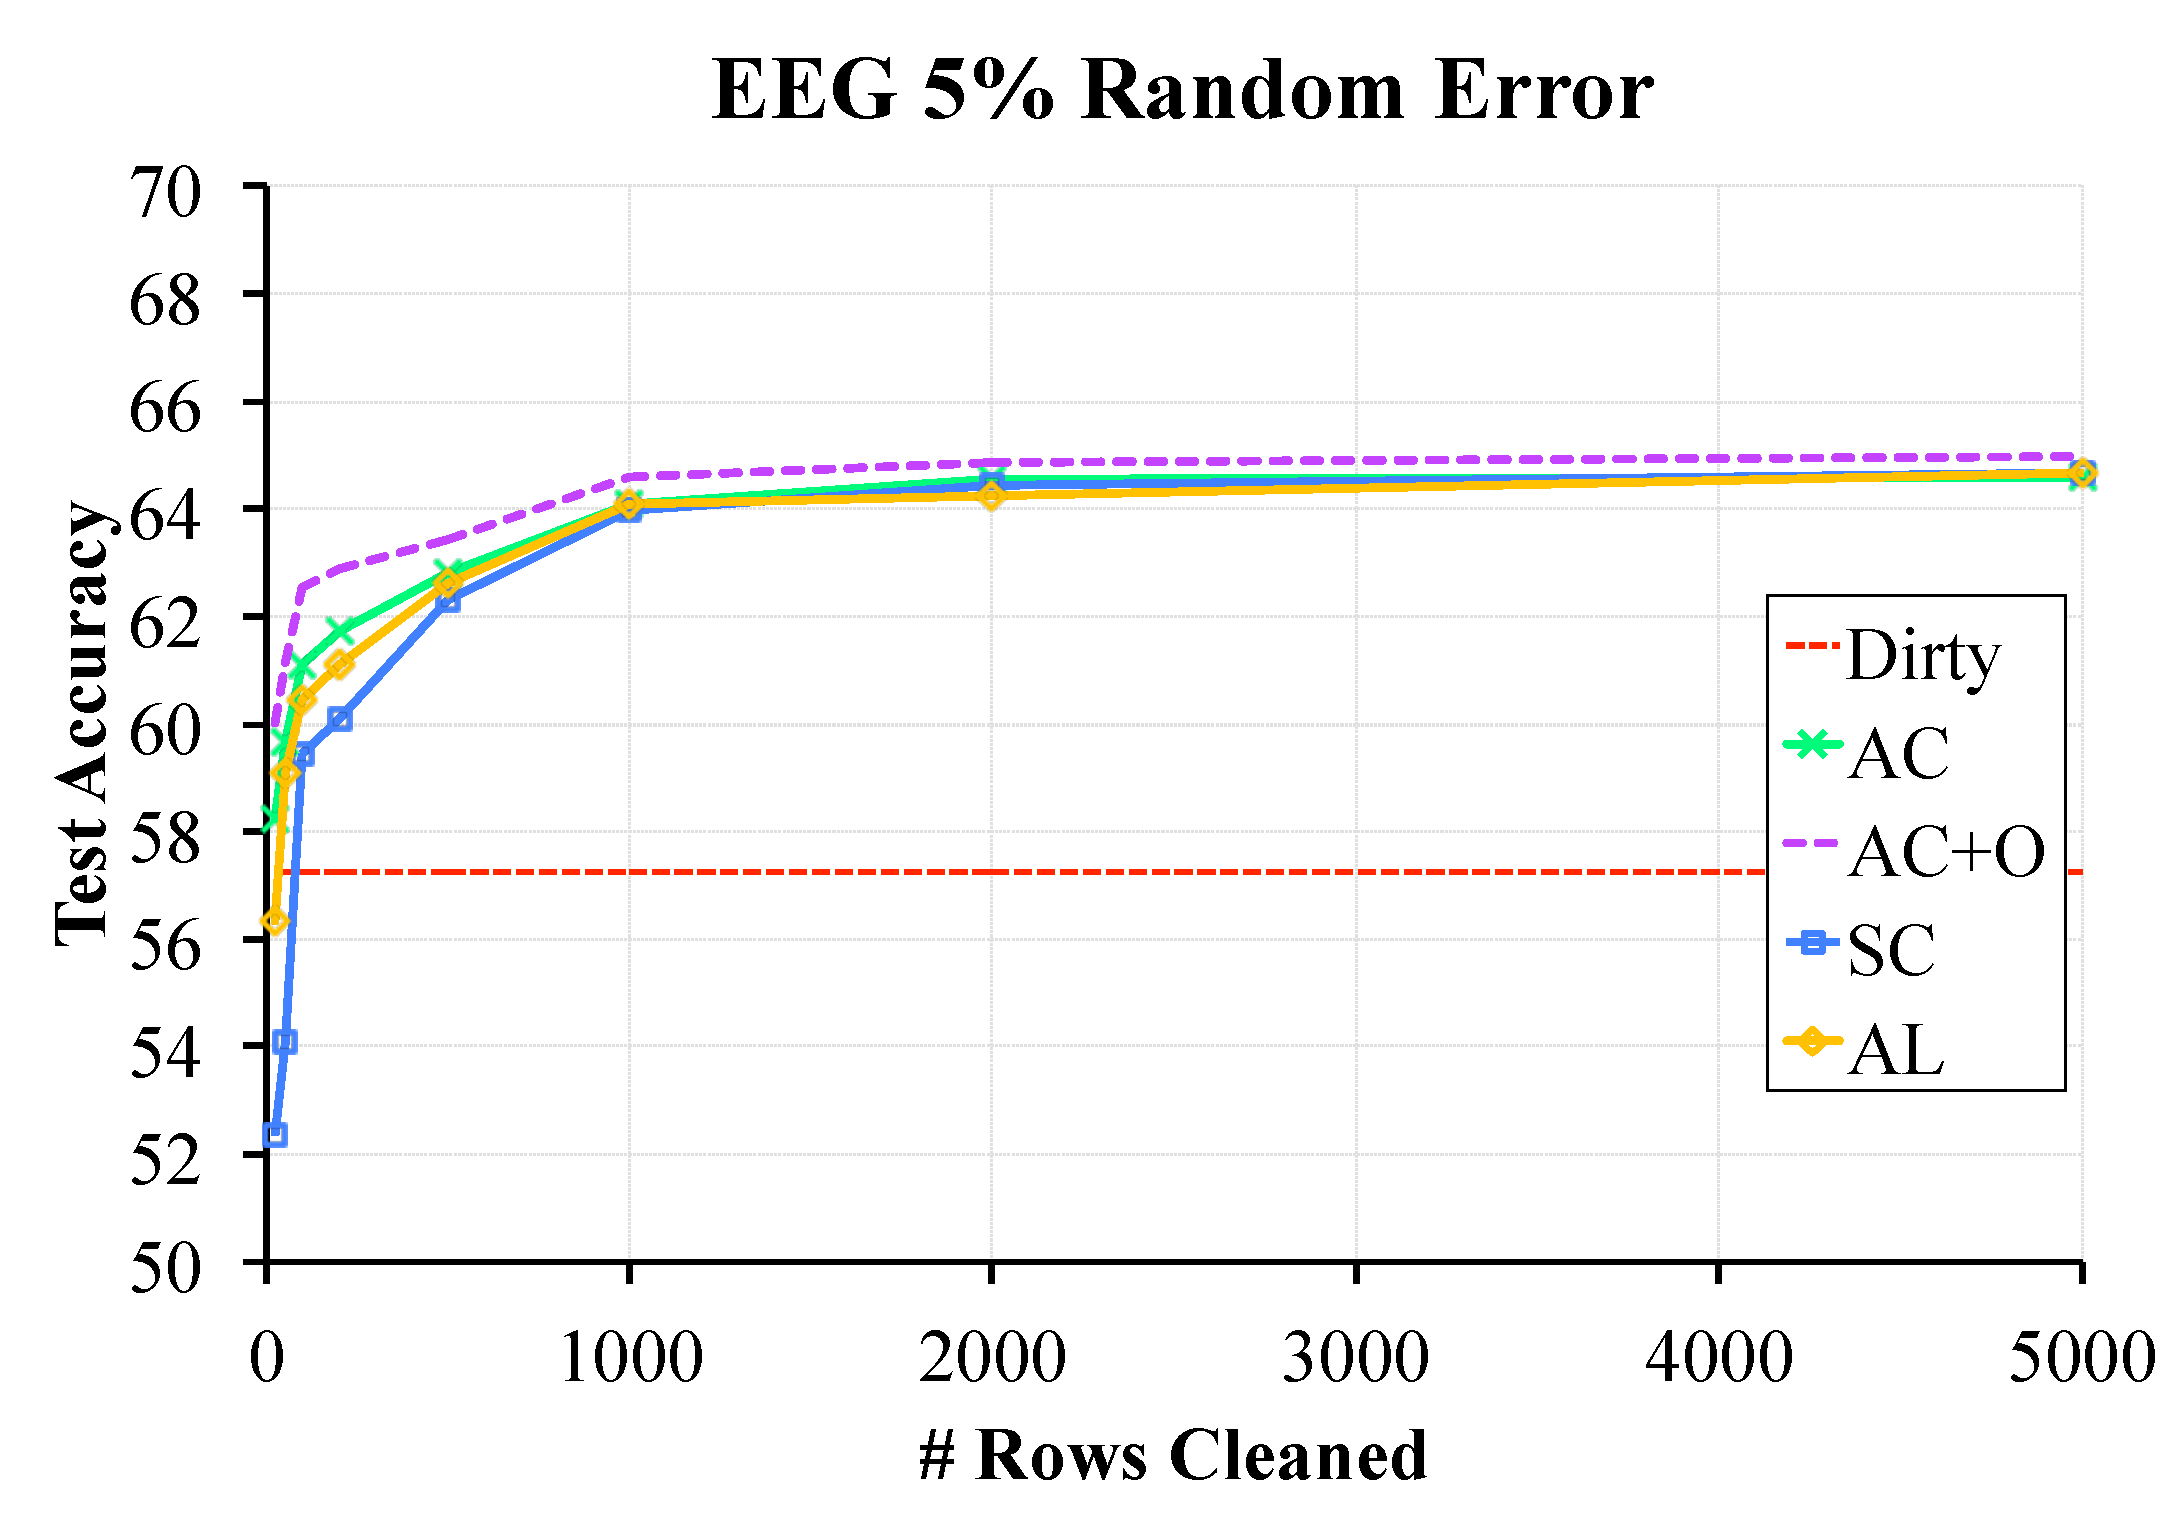
\includegraphics[scale=0.15]{exp/exp3cc.pdf}
 \caption{\sys converges with a smaller sample size to the maximum test accuracy in comparison to Active Learning and SampleClean. \label{prio-tperf}}
\end{figure*}

\subsection{Experiment 3. Predicates vs. Classification}

\subsubsection{3a. Basic Performance}
In the next set of experiments, we explore the error partitioning in more detail.
We presented two models for error sampling, one where we are given a set of candidate dirty records through a predicate and one where we have to learn this predicate as we clean.
In Figure \ref{pred-perf}, we overlay the convergence plots in the previous experiments with a curve (denoted by AC+C) that represents \sys using a classifier instead of an error predicate.
We use an SVM classifier to predict errors.
We find an interesting tradeoff where initially \sys is comparable to Active Learning (explanation for why seen in Figure \ref{opts}), as our classifier becomes more effective the partitioning improves the performance.

\begin{figure}[t]
\centering
 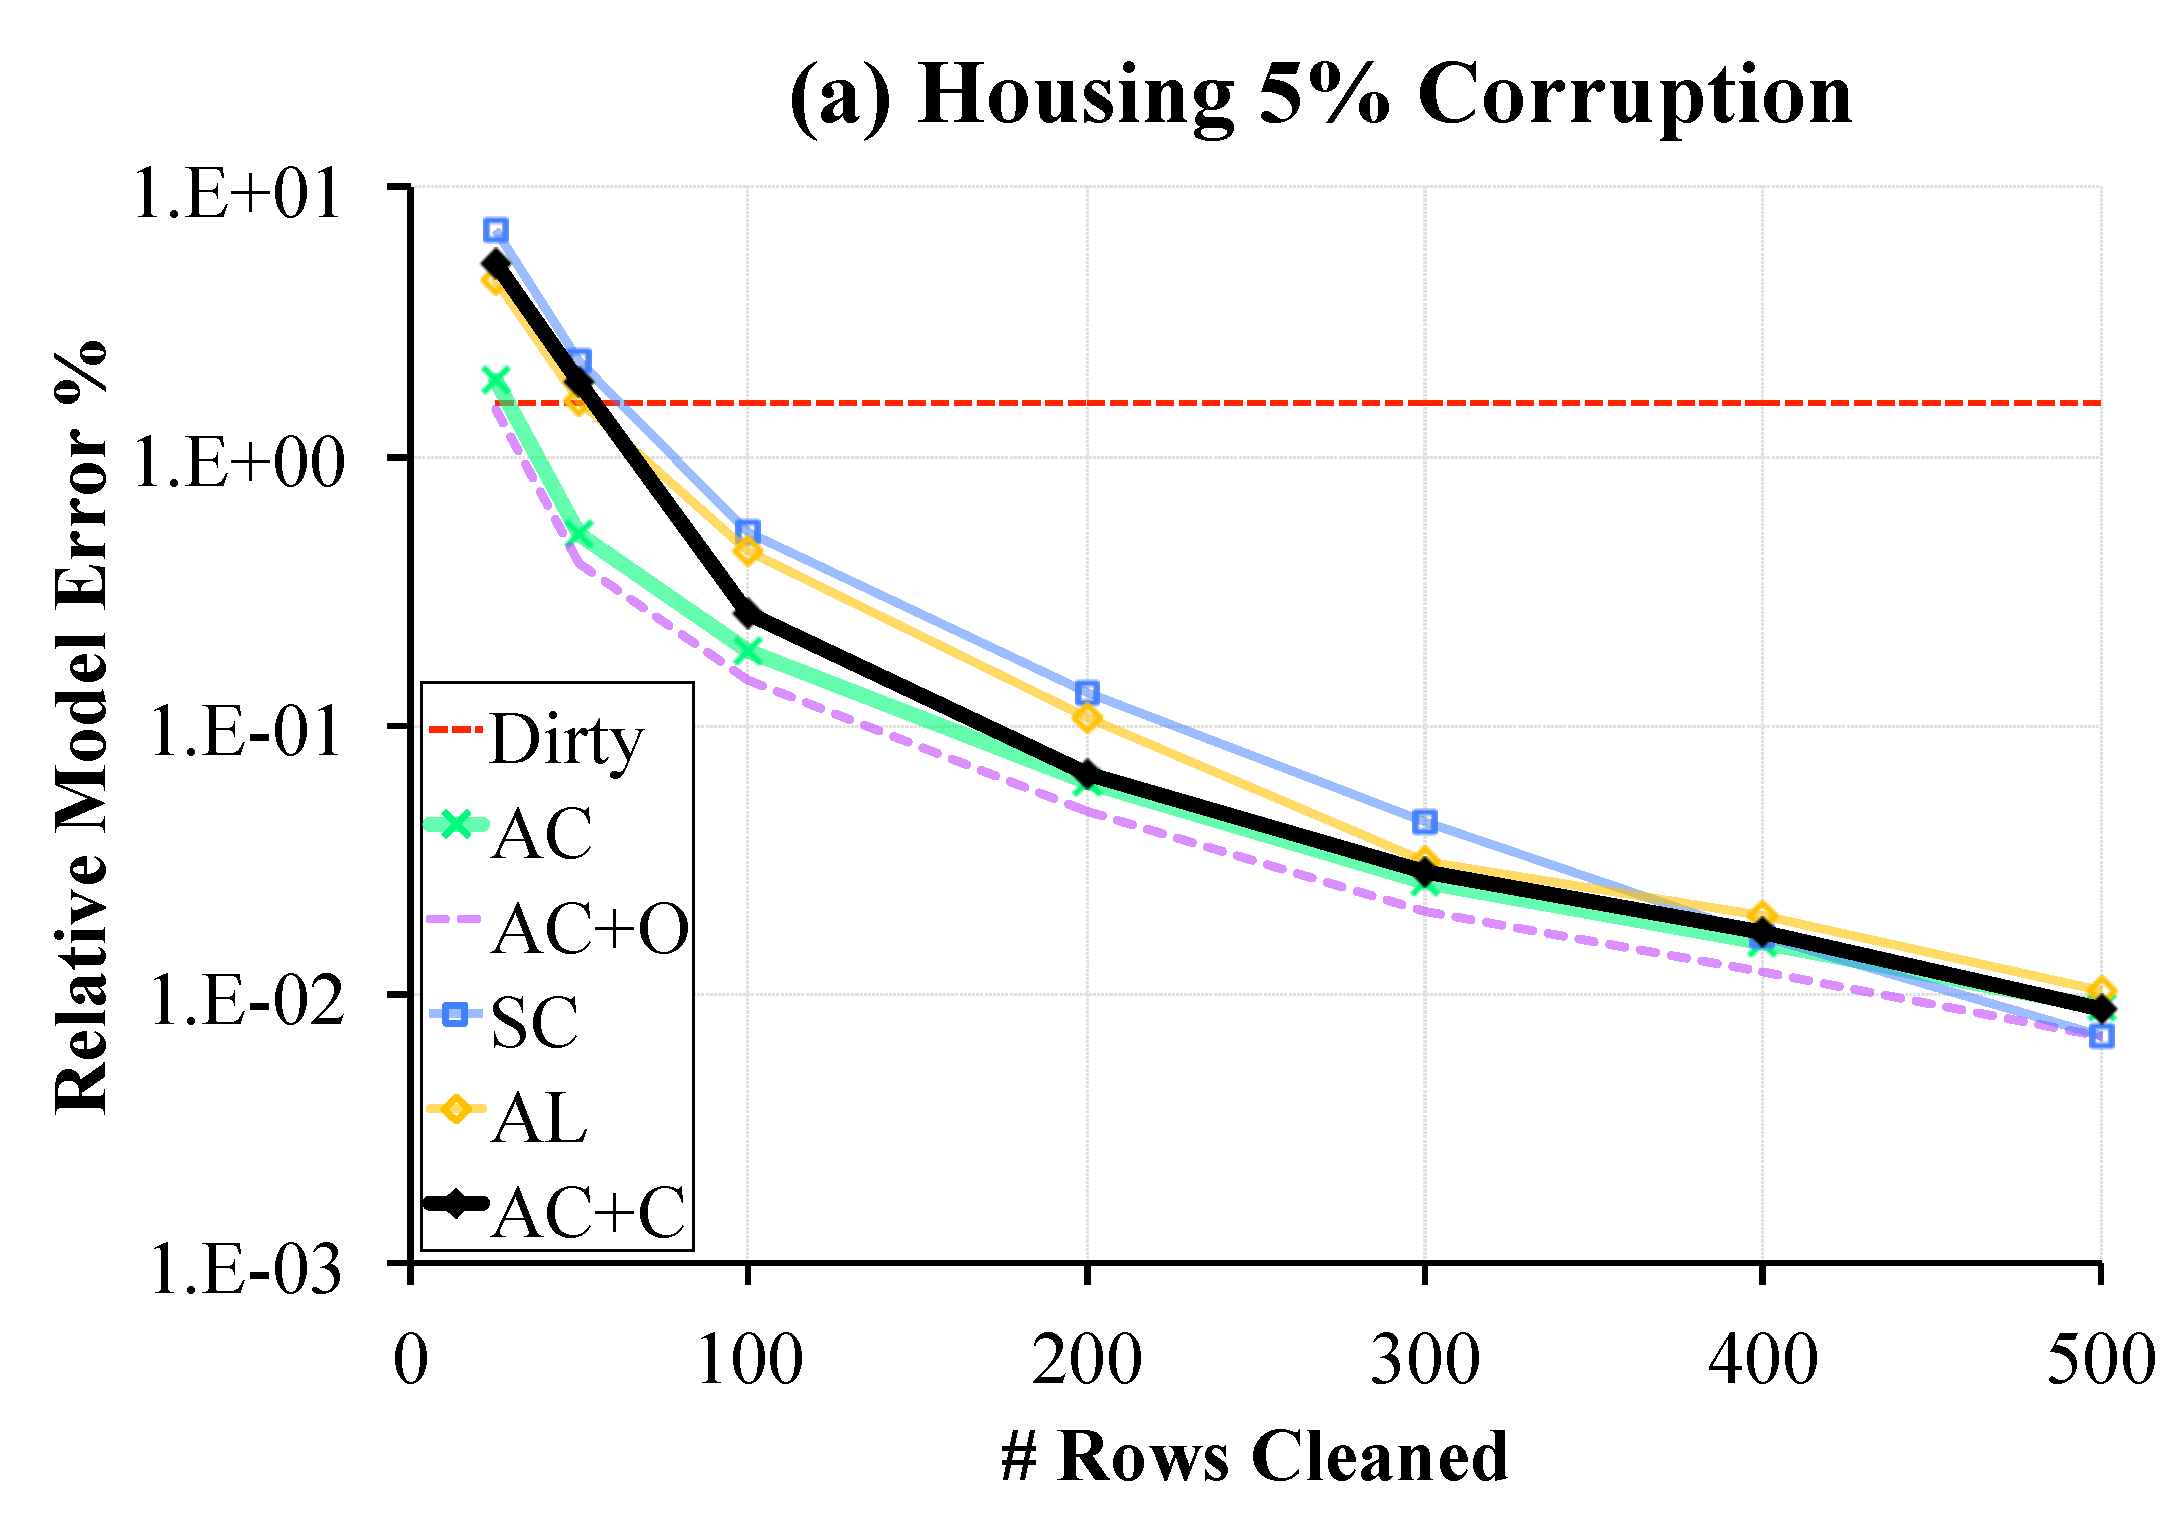
\includegraphics[width=0.48\columnwidth]{exp/exp11a.pdf}
 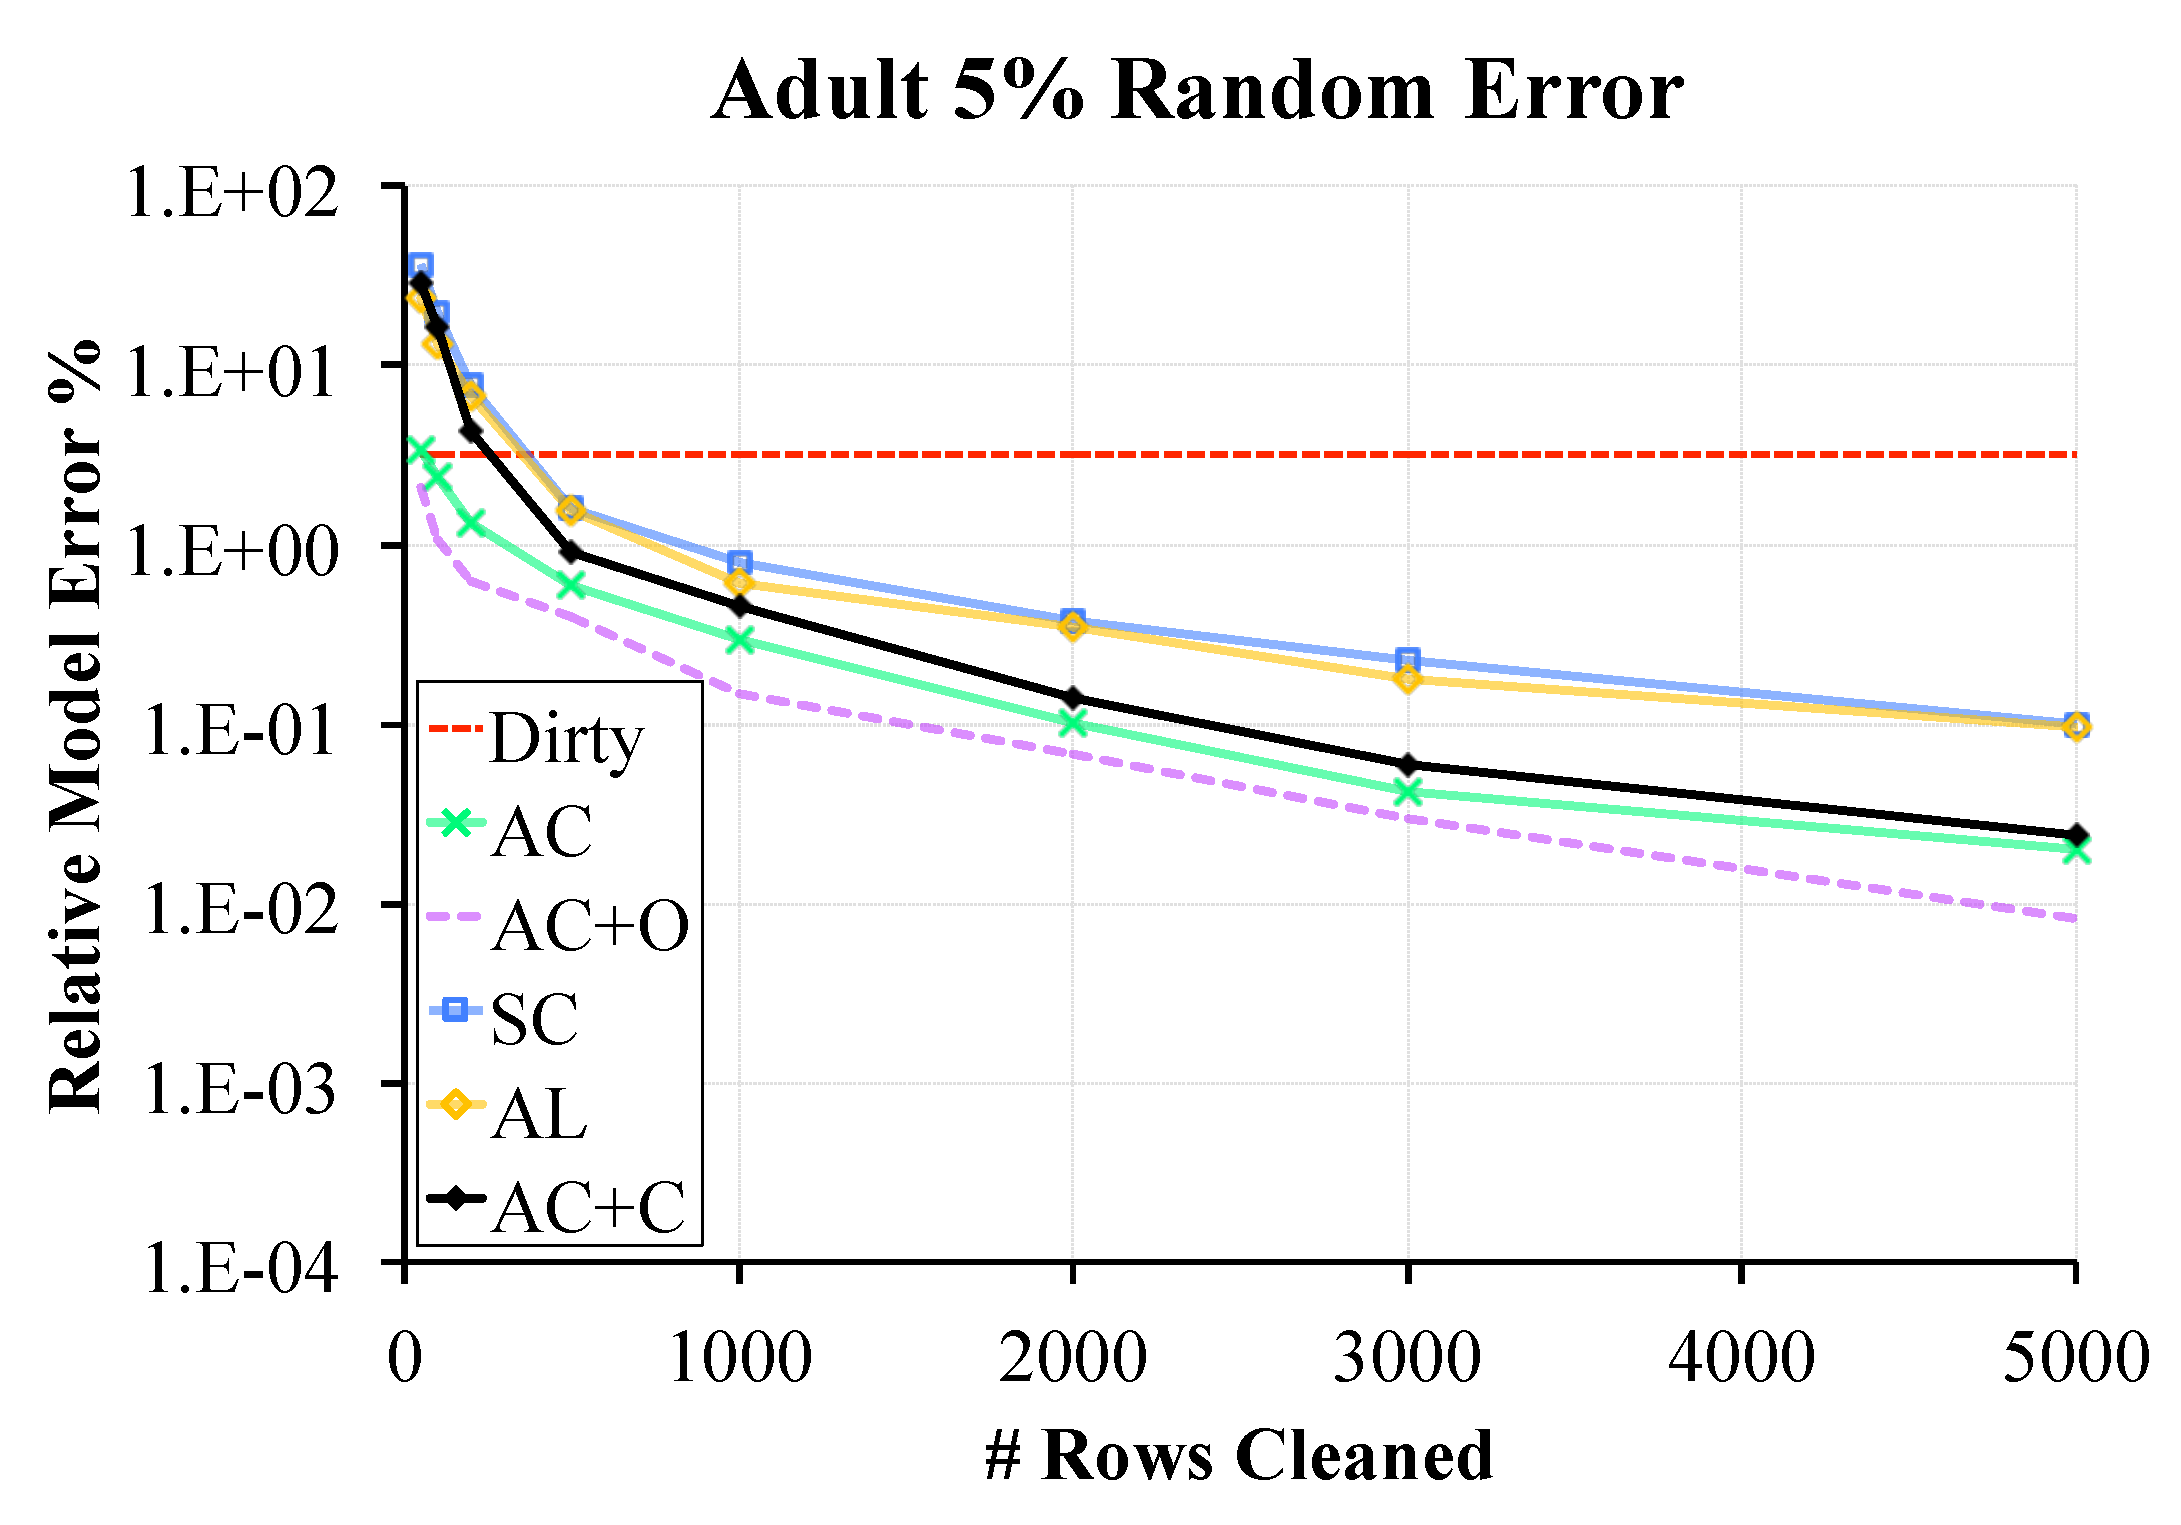
\includegraphics[width=0.48\columnwidth]{exp/exp11b.pdf}
 \caption{While initially \sys is comparable in performance to Active Learning, as the classifier improves, \sys converges faster than Active Learning and SampleClean. \label{pred-perf}}
\end{figure}

\subsubsection{3b. Classifiable Errors}
Using a classifier to partition errors depends on errors that can be classified.
For example, random errors that look like other data may be hard to learn.
As errors become more random, the classifier becomes increasingly erroneous.
We run an experiment where we start with the systematic errors described earlier.
With probability $p$, we increasingly make these errors more random.
We compare these results to AC-P where we do not partition the errors.
In Figure \ref{tradeoffs2}, we plot the error reduction using a classifier.
We find that when errors are about 40\% random then we reach a break even point
where the user is better of not partitiong the data since the errors introduced by incorrect classification are more than the error reductions.

\begin{figure}[ht!]
\centering
 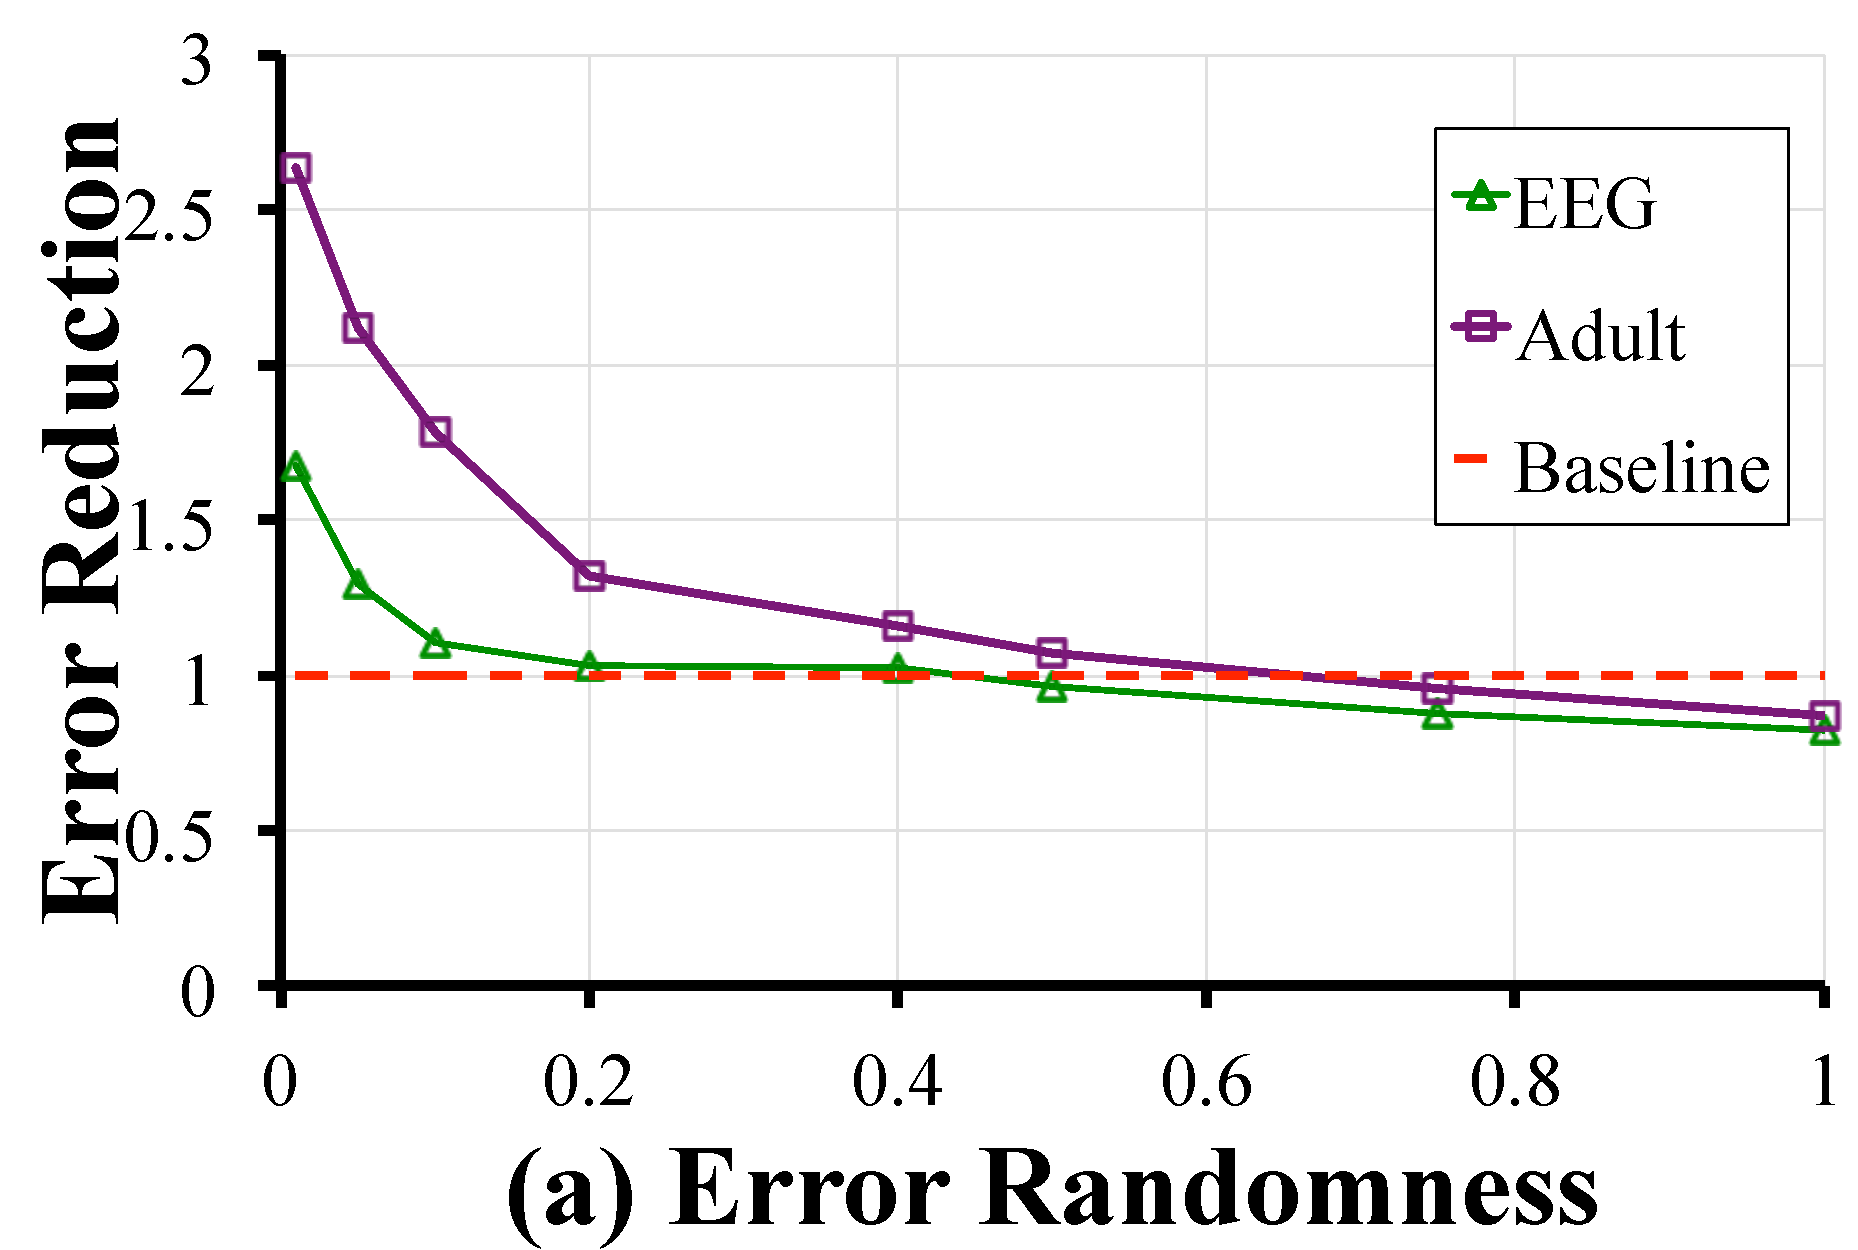
\includegraphics[scale=0.13]{exp/exp5a.pdf}
 \caption{Errors that are less random are easier to classify, and lead to more significant reductions in relative model error. \label{tradeoffs2}}
\end{figure}

\subsection{Experiment 4. Price of a Scan}
In our fourth set of experiments, we evaluate one of the computational premises of our work.
We argue that the price of a scan of data is cheap compared to data cleaning.
The overheads of partioning the dirty and clean data and calculating the sampling distribution should be small in comparison to the faster convergence of our model.
\reminder{How do we quantify the costs of data cleaning?} 

\subsection{Real Scenarios}
\reminder{Value Filling: MNIST}

\begin{figure*}[t]
\centering
 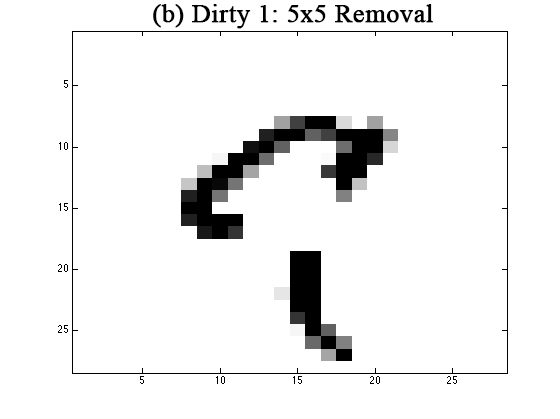
\includegraphics[scale=0.25]{exp/5x5removal.png}
 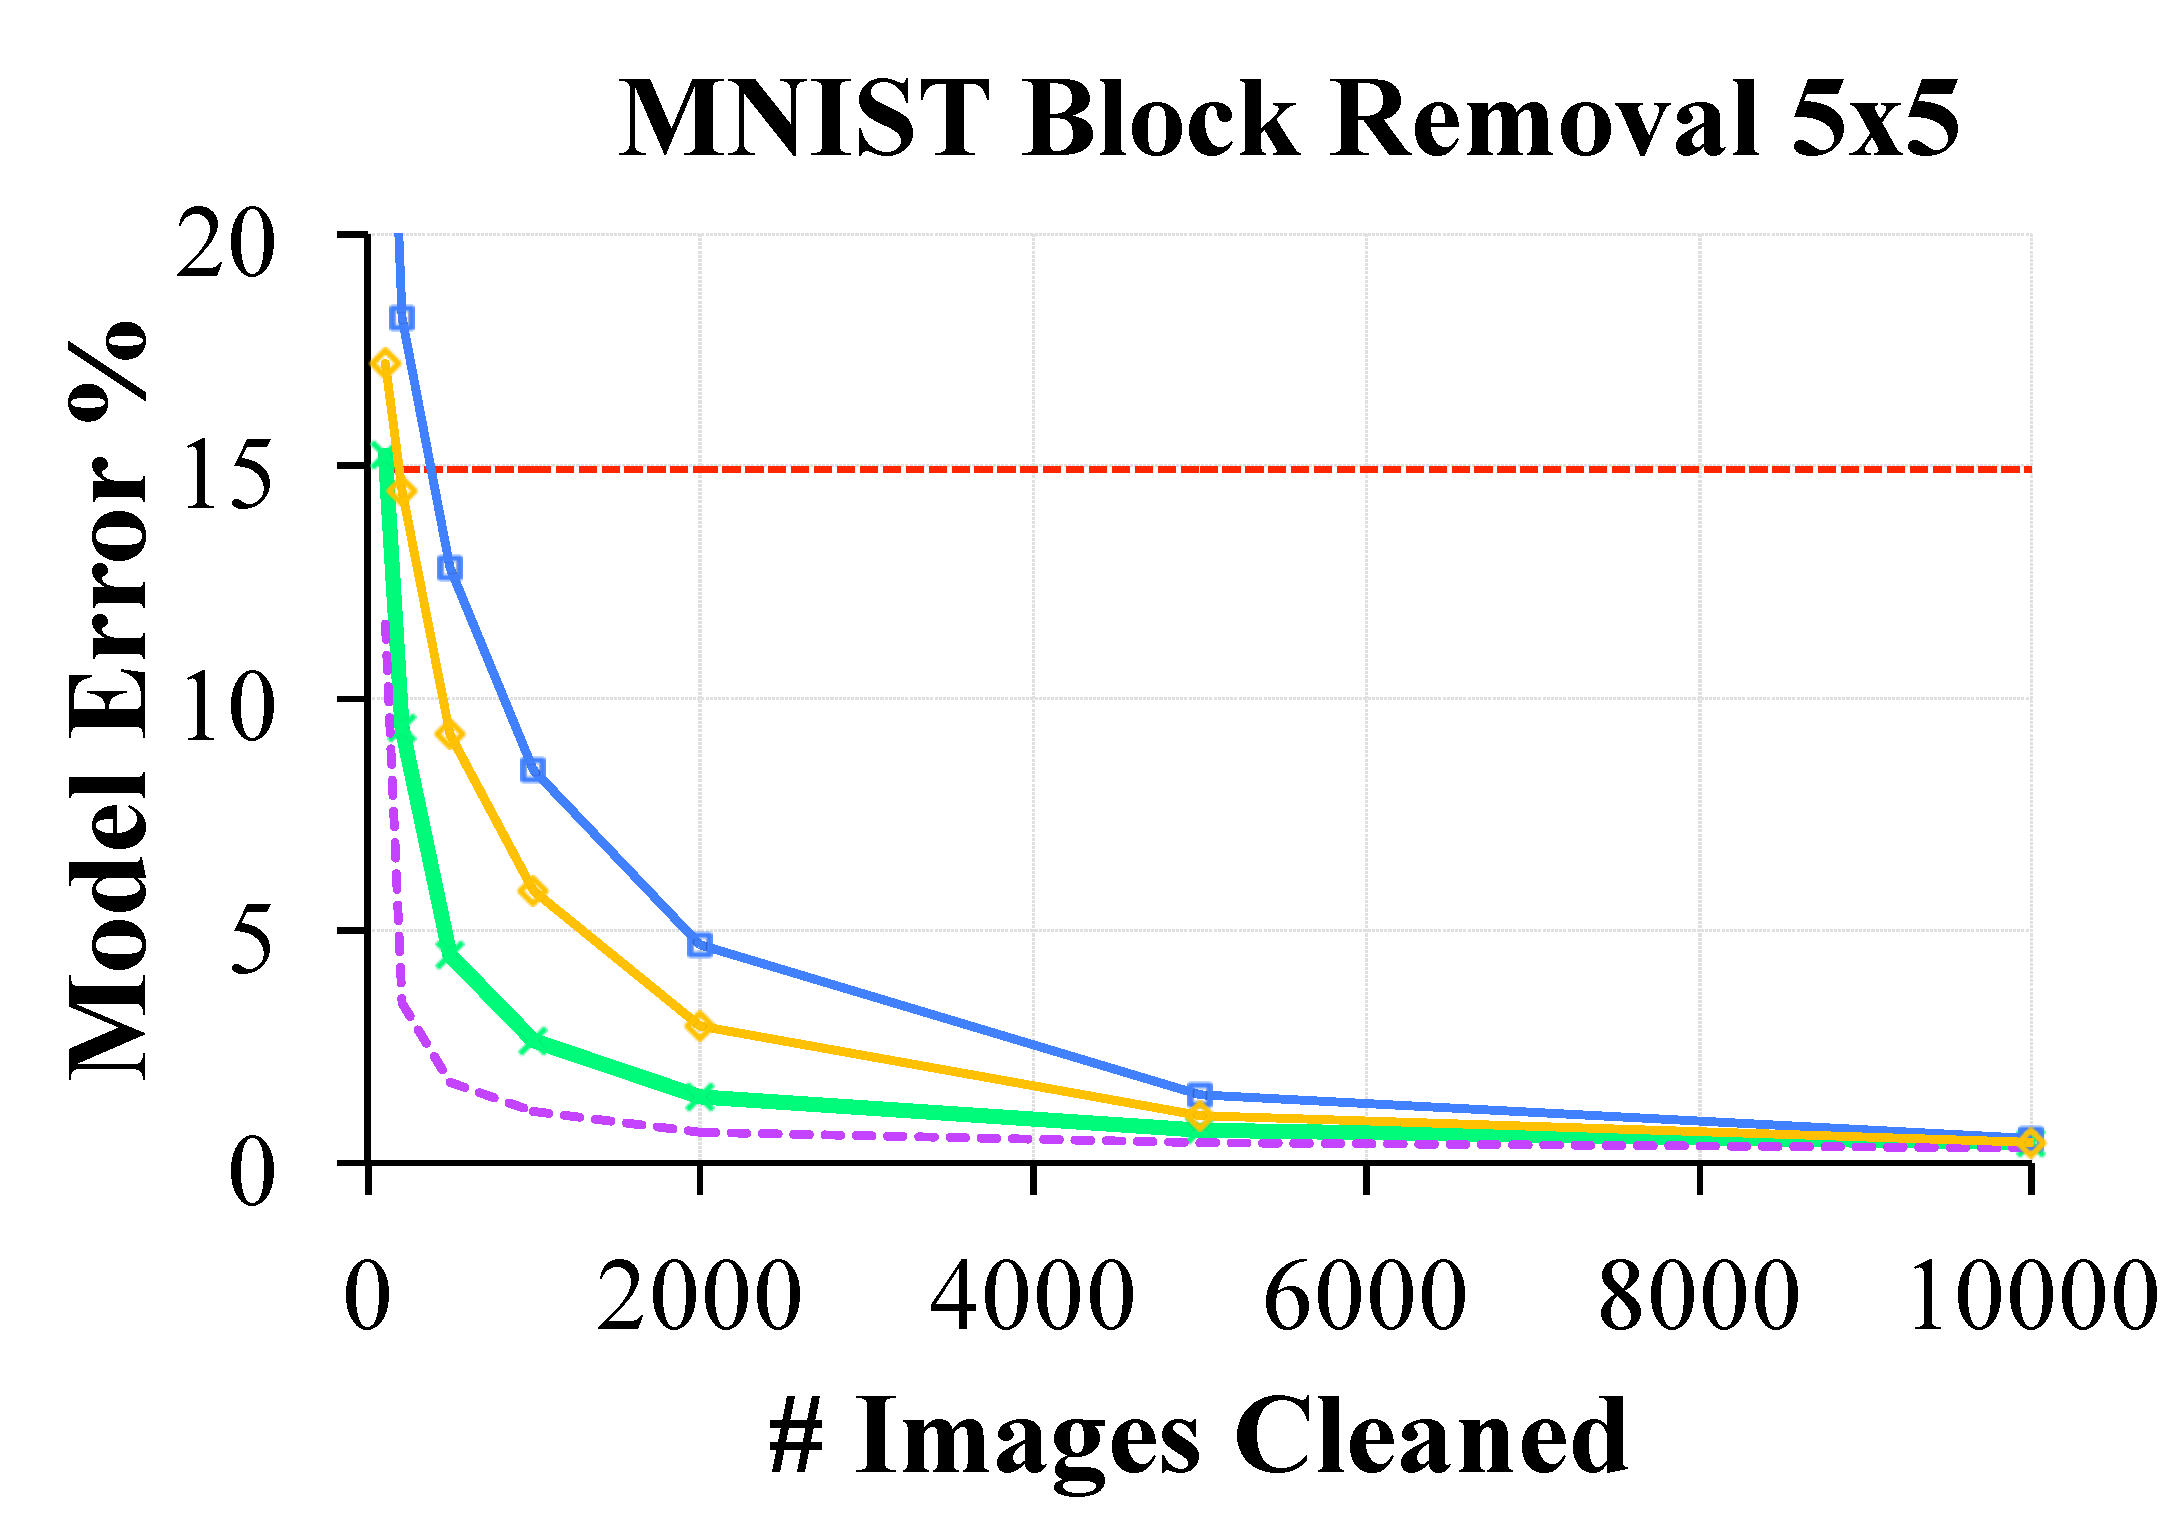
\includegraphics[scale=0.15]{exp/exp7a.pdf}
 \caption{One experiment with MNIST}
\end{figure*}

\reminder{CFD: Adult}
\vspace{-1em}
\section{Related Work}
\noindent \textbf{Data Cleaning and Databases: } There are also several recent results in data cleaning that we would like to highlight. 
Progressive data cleaning methodologies have been proposed, however, these techniques tend to be application agnostic \cite{mayfield2010eracer}.
Altowim et al. proposed a framework for progressive entity resolution \cite{altowim2014progressive}. 
Volkovs et al. explored a related topic of maintaining data cleaning rules that change over time \cite{volkovs2014continuous}. 
Recently, in works such as SampleClean \cite{wang1999sample}, the application (i.e., queries) are used to inform data cleaning methodology.
When the workload is made up of aggregate queries, cleaning samples of data may suffice. 
Similarly, Bergman et al. explore the problem of query-oriented data cleaning \cite{DBLP:conf/sigmod/BergmanMNT15}. Given a query they clean data relevant to that query. 
Bergman et al. does not explore the Machine Learning applications studied in this work.
Deshpande et al. studied data acquisition in sensor networks \cite{deshpande2004model}. They explored value of information based prioritization of data acquisition for estimating aggregate queries of sensor readings.
Similarly, Jeffery et al. \cite{DBLP:conf/pervasive/JefferyAFHW06} explored similar prioritization based on value of information.
We see this work as pushing prioritization further down the pipeline to the end analytics.
Finally, incremental optimization methods like SGD have a connection to incremental materialized view maintenance as the argument for incremental maintenance over recomputation is similar (i.e., relatively sparse updates).
Krishnan et al. explored how samples of materialized views can be maintained similar to how models are updated with a sample of clean data in this work \cite{krishnan2015svc}

\vspace{0.5em}

\noindent \textbf{Stochastic Optimization and Active Learning: } Zhao and Tong recently proposed using importance sampling in conjunction with stochastic gradient descent \cite{zhao2014stochastic}. 
The ideas applied in \sys are well rooted in the Machine Learning and Optimization literature, and we apply these ideas to the data cleaning problem. 
This line of work builds on prior results in linear algebra that show that some matrix columns are more informative than others \cite{drineas2012fast}, and Active Learning which shows that some labels are more informative that others \cite{settles2010active}.
Active Learning largely studies the problem of label acquisition \cite{settles2010active},
and recently the links between Active Learning and Stochastic optimization have been studied \cite{guillory2009active}. 
We use the work in Guillory et al. to evaluate a state-of-the-art Active Learning technique against \sys.


\vspace{0.5em}

\noindent \textbf{Transfer Learning and Bias Mitigation: }  
\sys has a strong link to a field called Transfer Learning and Domain Adaptation \cite{pan2010survey}. The basic idea of Transfer Learning is that suppose a model is trained on a dataset $D$ but tested on a dataset $D'$. 
Much of the complexity and contribution of \sys comes from efficiently tuning such a process for expensive data cleaning applications -- costs not studied in Transfer Learning.
In robotics, Mahler et al. explored a calibration problem in which data was systematically corrupted \cite{DBLP:conf/case/MahlerKLSMKPWFAG14} and proposed a rule-based technique for cleaning data.
Other problems in bias mitigation (e.g., Krishnan et al. \cite{DBLP:conf/recsys/KrishnanPFG14}) have the same structure, systematically corrupted data that is feeding into a model.
In this work, we try to generalize these principles given a general dirty dataset, convex model, and data cleaning procedure.


\vspace{0.5em}

\noindent \textbf{Secure Learning: } Another relevant line of work is the work in private machine learning  \cite{wainwright2012privacy, duchi2013local}. Learning is performed on a noisy variant of the data which mitigates privacy concerns, embracing the error rather than correcting for it. \sys is also related to work in adversarial learning \cite{nelson2012query}, where the goal is to make models robust to adversarial data manipulation.
This line of work has extensively studied methodologies for making models private to external queries and robust to malicious labels \cite{xiaofeature}, but the data cleaning problem explores more general corruptions than just malicious labels.
One widely applied technique in this field is reject-on-negative impact, which essentially, discards data that reduces the loss function--which will not work when we do not have access to the true loss function (only the ``dirty loss"). 



\vspace{2em}\section{Discussion and Future Work}
The experimental results suggest the following conclusions about \sys: (1) when the data corruption rate is relatively small (e.g., 5\%), \sys cleans fewer records than Active Learning or Sample Clean to achieve the same model accuracy, (2) all of the optimizations in \sys (importance sampling, detection, and estimation) lead to significantly more accurate models at small sample sizes, (3) only when corruption rates are very severe (e.g. 50\%) , SampleClean out performs \sys, and (4) two real-world scenarios demonstrate similar accuracy improvements where \sys returns significantly more accurate models than SampleClean or Active Learning for the same number of records cleaned.

There are also a few additional points for discussion.
\sys provides guarantees for training error on models trained with progressive data cleaning, however, there are no such guarantees on test error. 
This work focuses on the problem where an analyst has a large amount of dirty data and would like explore data cleaning and predictive models on this dataset.
By providing the analyst more accurate model estimates, the value of different data cleaning techniques can be judged without having to clean the entire dataset.
However, this problem is distinct from the model deployment problem, which we hope to explore in more detail in future work.
It implicitly assumes that when the model is deployed, it will be applied in a setting where the test data is also clean.
Training on clean data, and testing on dirty data, defeats the purpose of data cleaning and can lead to unreliable predictions.

As the experiments clearly show, \sys is not strictly \emph{better} than Active Learning or Sample Clean.
\sys is optimized for a specific design point of sparse errors and small sample sizes, and the empirical results suggest it returns more accurate models in this setting.
As sample sizes and error rates increase, the benefits of \sys are reduced.
Another consideration for future work is automatically selecting alternative techniques when \sys is expected to perform poorly.

Beyond these limitations, there are several exciting new avenues for future work.
The data cleaning models explored in this work can be extended to handle non-uniform costs, where different errors have a different cleaning cost.
Next, the empirical success of Deep Learning has led to increasing industry and research adoption of non-convex losses in many tasks that were traditionally served by convex models.
In future work, we hope to explore how we can integrate with such frameworks.



\section{Conclusion}
The growing popularity of predictive models (e.g., classifiers) in data analytics adds additional challenges in managing dirty data with mixing dirty and clean data, sensitivity to sampling, and sparsity.
\sys is a framework that utilizes data cleaning to mitigate systematic errors with progressive data cleaning.
The key insight is that an important class of predictive models, called convex loss models (e.g., linear regression and SVMs), can be simultaneously trained and cleaned.
Consequently, there are provable guarantees on the convergence and error bounds of \sys.  
\sys also includes numerous optimizations such as: using the information from the model to inform data cleaning on samples, dirty data detection to avoid sampling clean data, and batching together updates on already clean data.
The experimental results are promising as they suggest that these optimizations can significantly reduce data cleaning costs when errors are sparse and cleaning budgets are small.
Techniques such as Active Learning and SampleClean are not optimized for the sparse low-budget setting, and \sys achieves models of similar accuracy for significantly less records cleaned.

%\input{outlier.tex}
%\input{analysis.tex}
%\section{Experiments}
There are a number of different axes on which we can evaluate \sys.
First, we take real datasets and generate various types of errors to illustrate the value of data cleaning in comparison to robust statistical techniques.
Next, we explore different prioritization and model update schemes for data cleaning samples.
Finally, we evaluate \sys end-to-end in a number of real-world data cleaning scenarios.

\subsection{Experimental Setup and Notation}
Every experiment has two steps: data cleaning and model evaluation.
We evaluate the data cleaning on one metric:

\noindent\textbf{Cleaning Efficiency. } Let $K$ be the number of samples processed by the algorithm, and $K'$ be the number of samples that were actually dirty. The cleaning efficiency is $\frac{K'}{K}$.

In our experiments, we explore three classification models: L1-Hinge Loss SVM, Logistic Regression, and Thresholded Linear Regression.
We evaluate the trained models on the following metrics:

\noindent\textbf{Relative Model Error. } Let $\theta$ be the model trained on the dirty data, and let $\theta^*$ be the model trained on the same data if it was cleaned. Then the model error is defined as $\frac{\|\theta - \theta^*\|}{\|\theta^*\|}$.

\noindent\textbf{Testing Accuracy. } Let $\theta$ be the model trained on the dirty data, and let $\theta^*$ be the model trained on the same data if it was cleaned. Let $T(\theta)$ be the out-of-sample testing accuracy when the dirty model is applied to the clean data, and $T(\theta^*)$ be the testing accuracy when the clean model is applied to the clean data. The testing error is defined as $T(\theta^*) - T(\theta)$

\subsubsection{Scenarios}
We apply these models in the following scenarios:

\noindent\textbf{Housing: } In this dataset, our task is to predict housing prices from 13 numerical and categorical covariates. There are 550 data points in this dataset. The model is a Logistic Regression classifier which predicts if the house price is greater than \$500k.

\noindent\textbf{Adult: } In this census dataset, our task is to predict the income bracket (binary) from 12 numerical and categorical covariates. There are 45552 data points in this dataset. We use a SVM classifier to predict the income bracket of the person.

\noindent\textbf{EEG: } In this dataset, our task is to predict the on set of a seizure (binary) from 15 numerical covariates. There are 14980 data points in this dataset. This dataset is unique because the classification is hard with linear predictors. The model that we use is a thresholded Linear Regression.

\noindent\textbf{MNIST: } In this dataset, our task is to classify 60,000 images of handwritten images into 10 categories. The unique part of this dataset is the featurized data consists of a 784 dimensional vector which includes edge detectors and raw image patches. We use this dataset to explore how we can corrupt the raw data to affect subsequent featurization. The model is an one-to-all multiclass SVM classifier. 

\subsection{Experiment 1. Effect of Cleaning}
Before we evaluate \sys, we first evaluate the benefits of cleaning on our 4 example datasets.
We first explore this problem without sampling to understand which types of errors are amenable to data cleaning and which are better suited for robust statistical techniques.
We compare 4 schemes: (1) cleaning, (2) adding an L2 regularizer tuned to maximal accuracy with a grid search, (3) discarding the dirty data, and (4) baseline of no cleaning.

We corrupted 5\% of the training examples in each dataset.
We corrupted these data in two different ways.

\noindent\textbf{Random errors: } We simulated high-magnitude random outliers. We select 5\% of the examples and features uniformly at random and replace a feature with 3 times the highest feature value.

\noindent\textbf{Systematic errors: } We simulated innocuous looking (but still incorrect) systematic errors. We trained the model on the clean data, find the most important feature (highest weighted). We sort examples but this feature and corrupt the top 5\% of examples with the mean value for that feature.

\begin{figure}[ht!]
\centering
 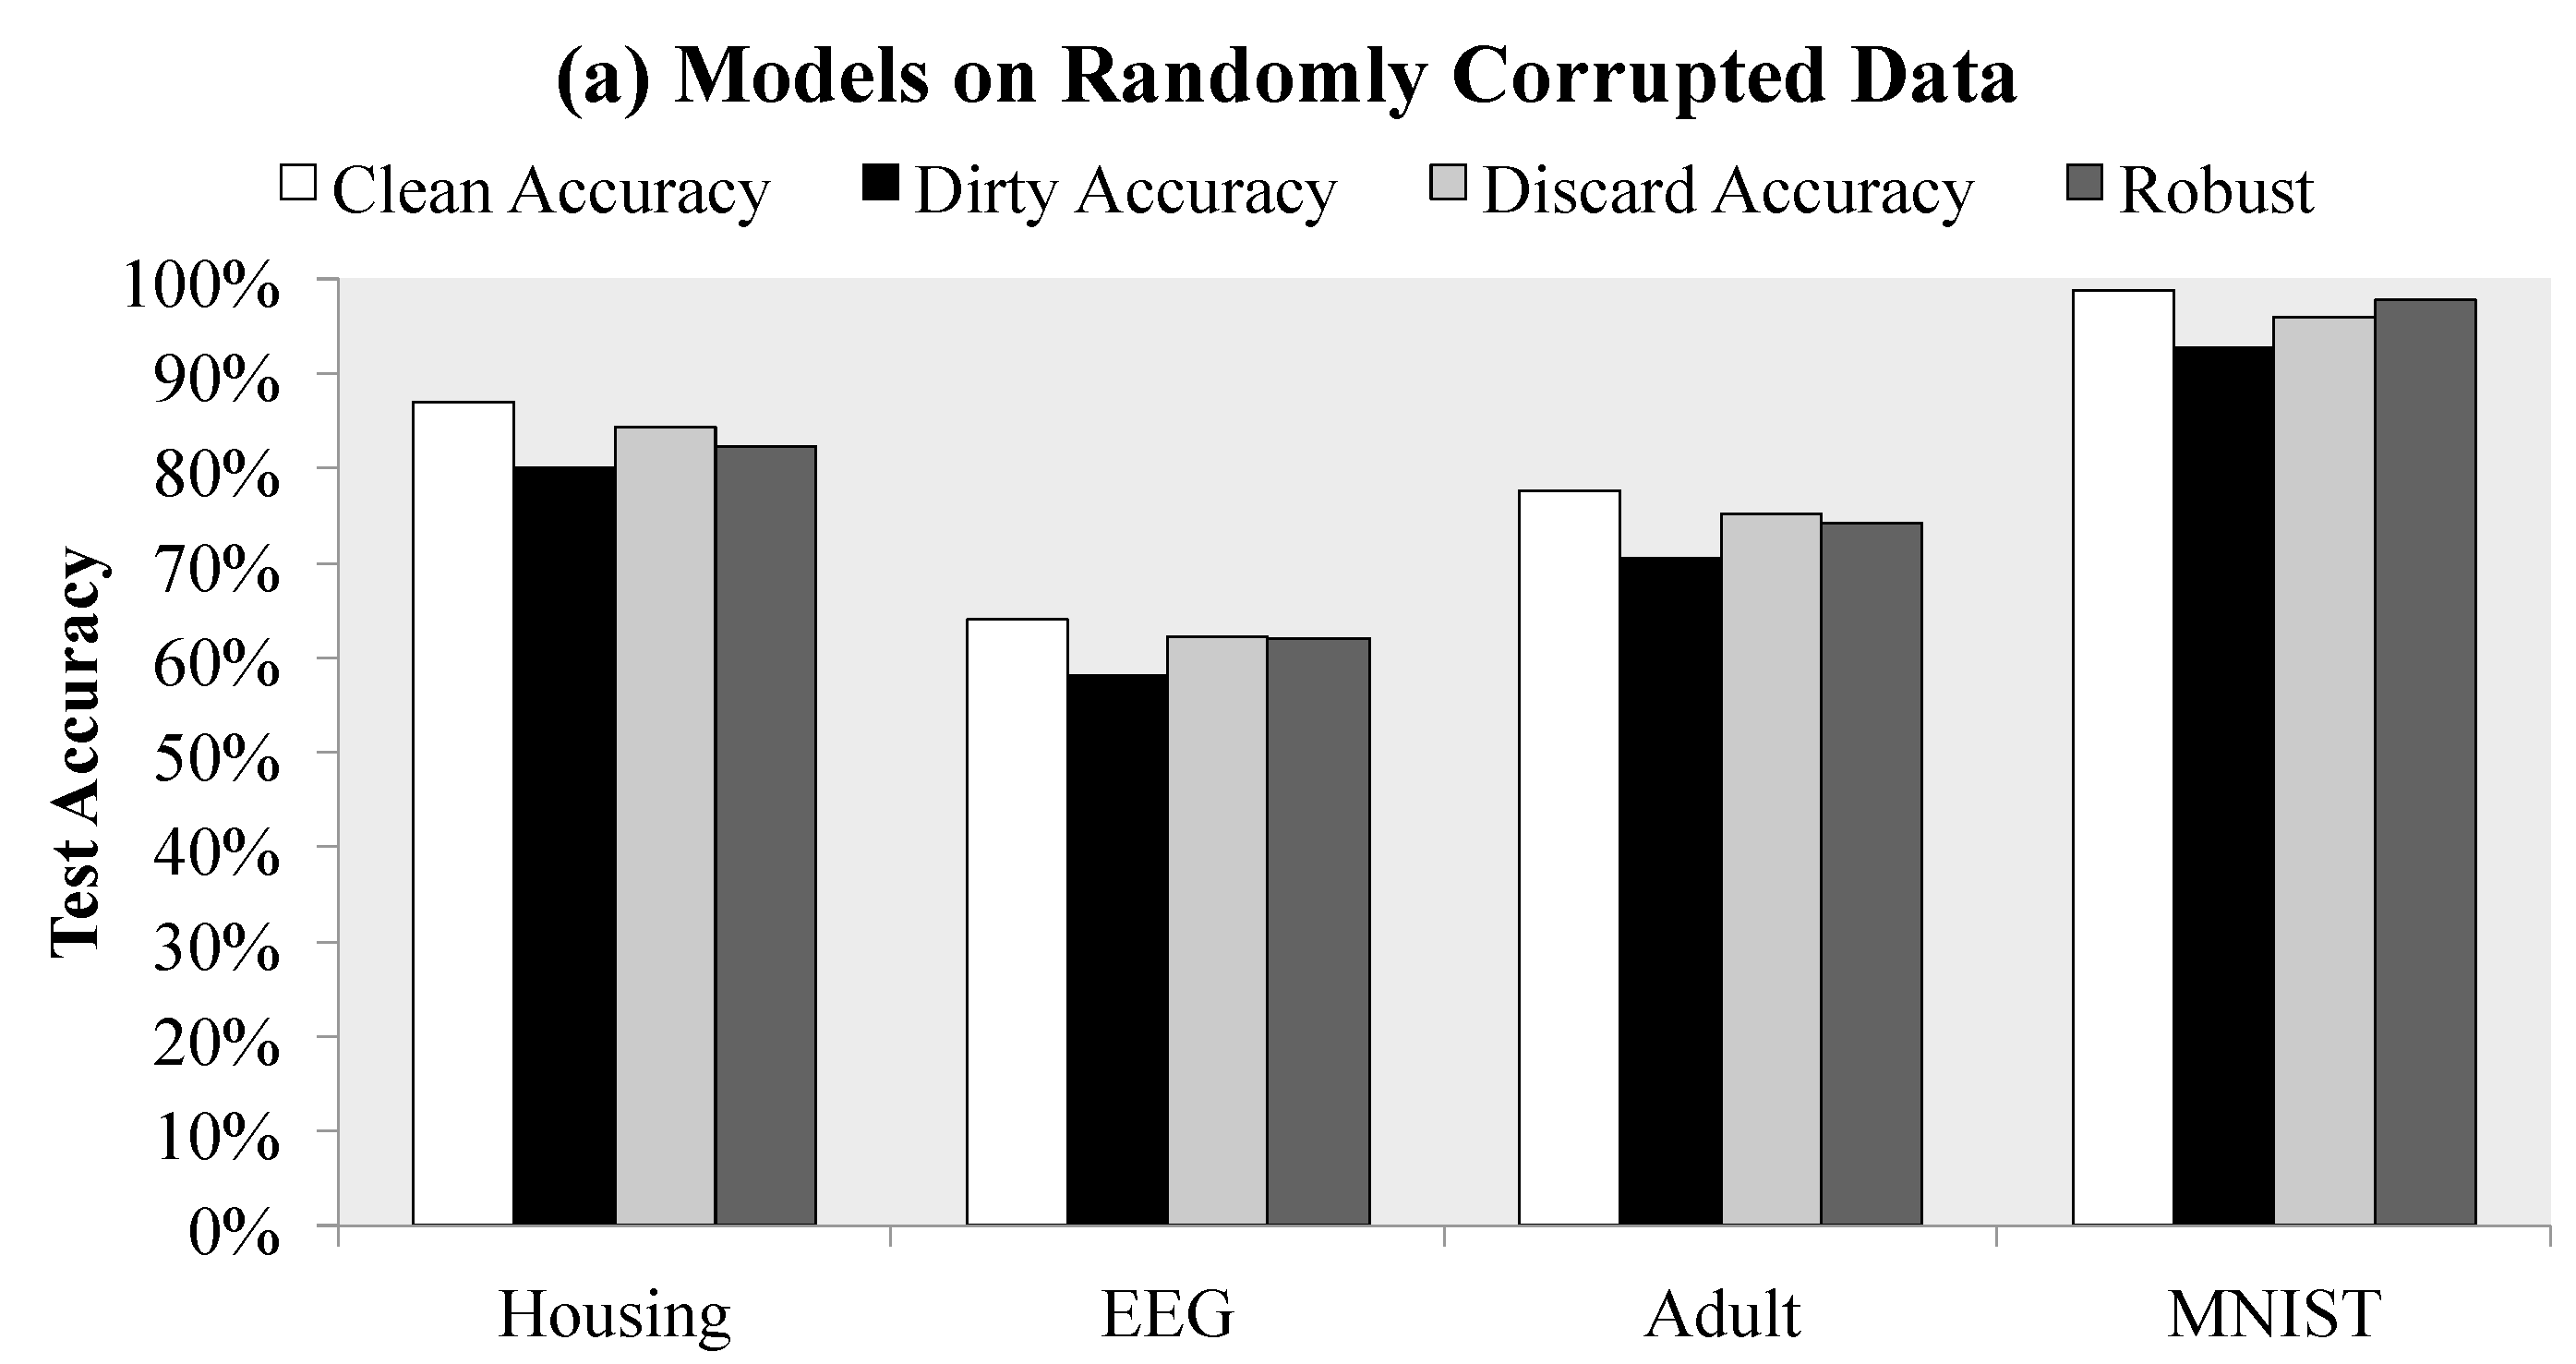
\includegraphics[width=0.8\columnwidth]{exp/exp2.pdf}
 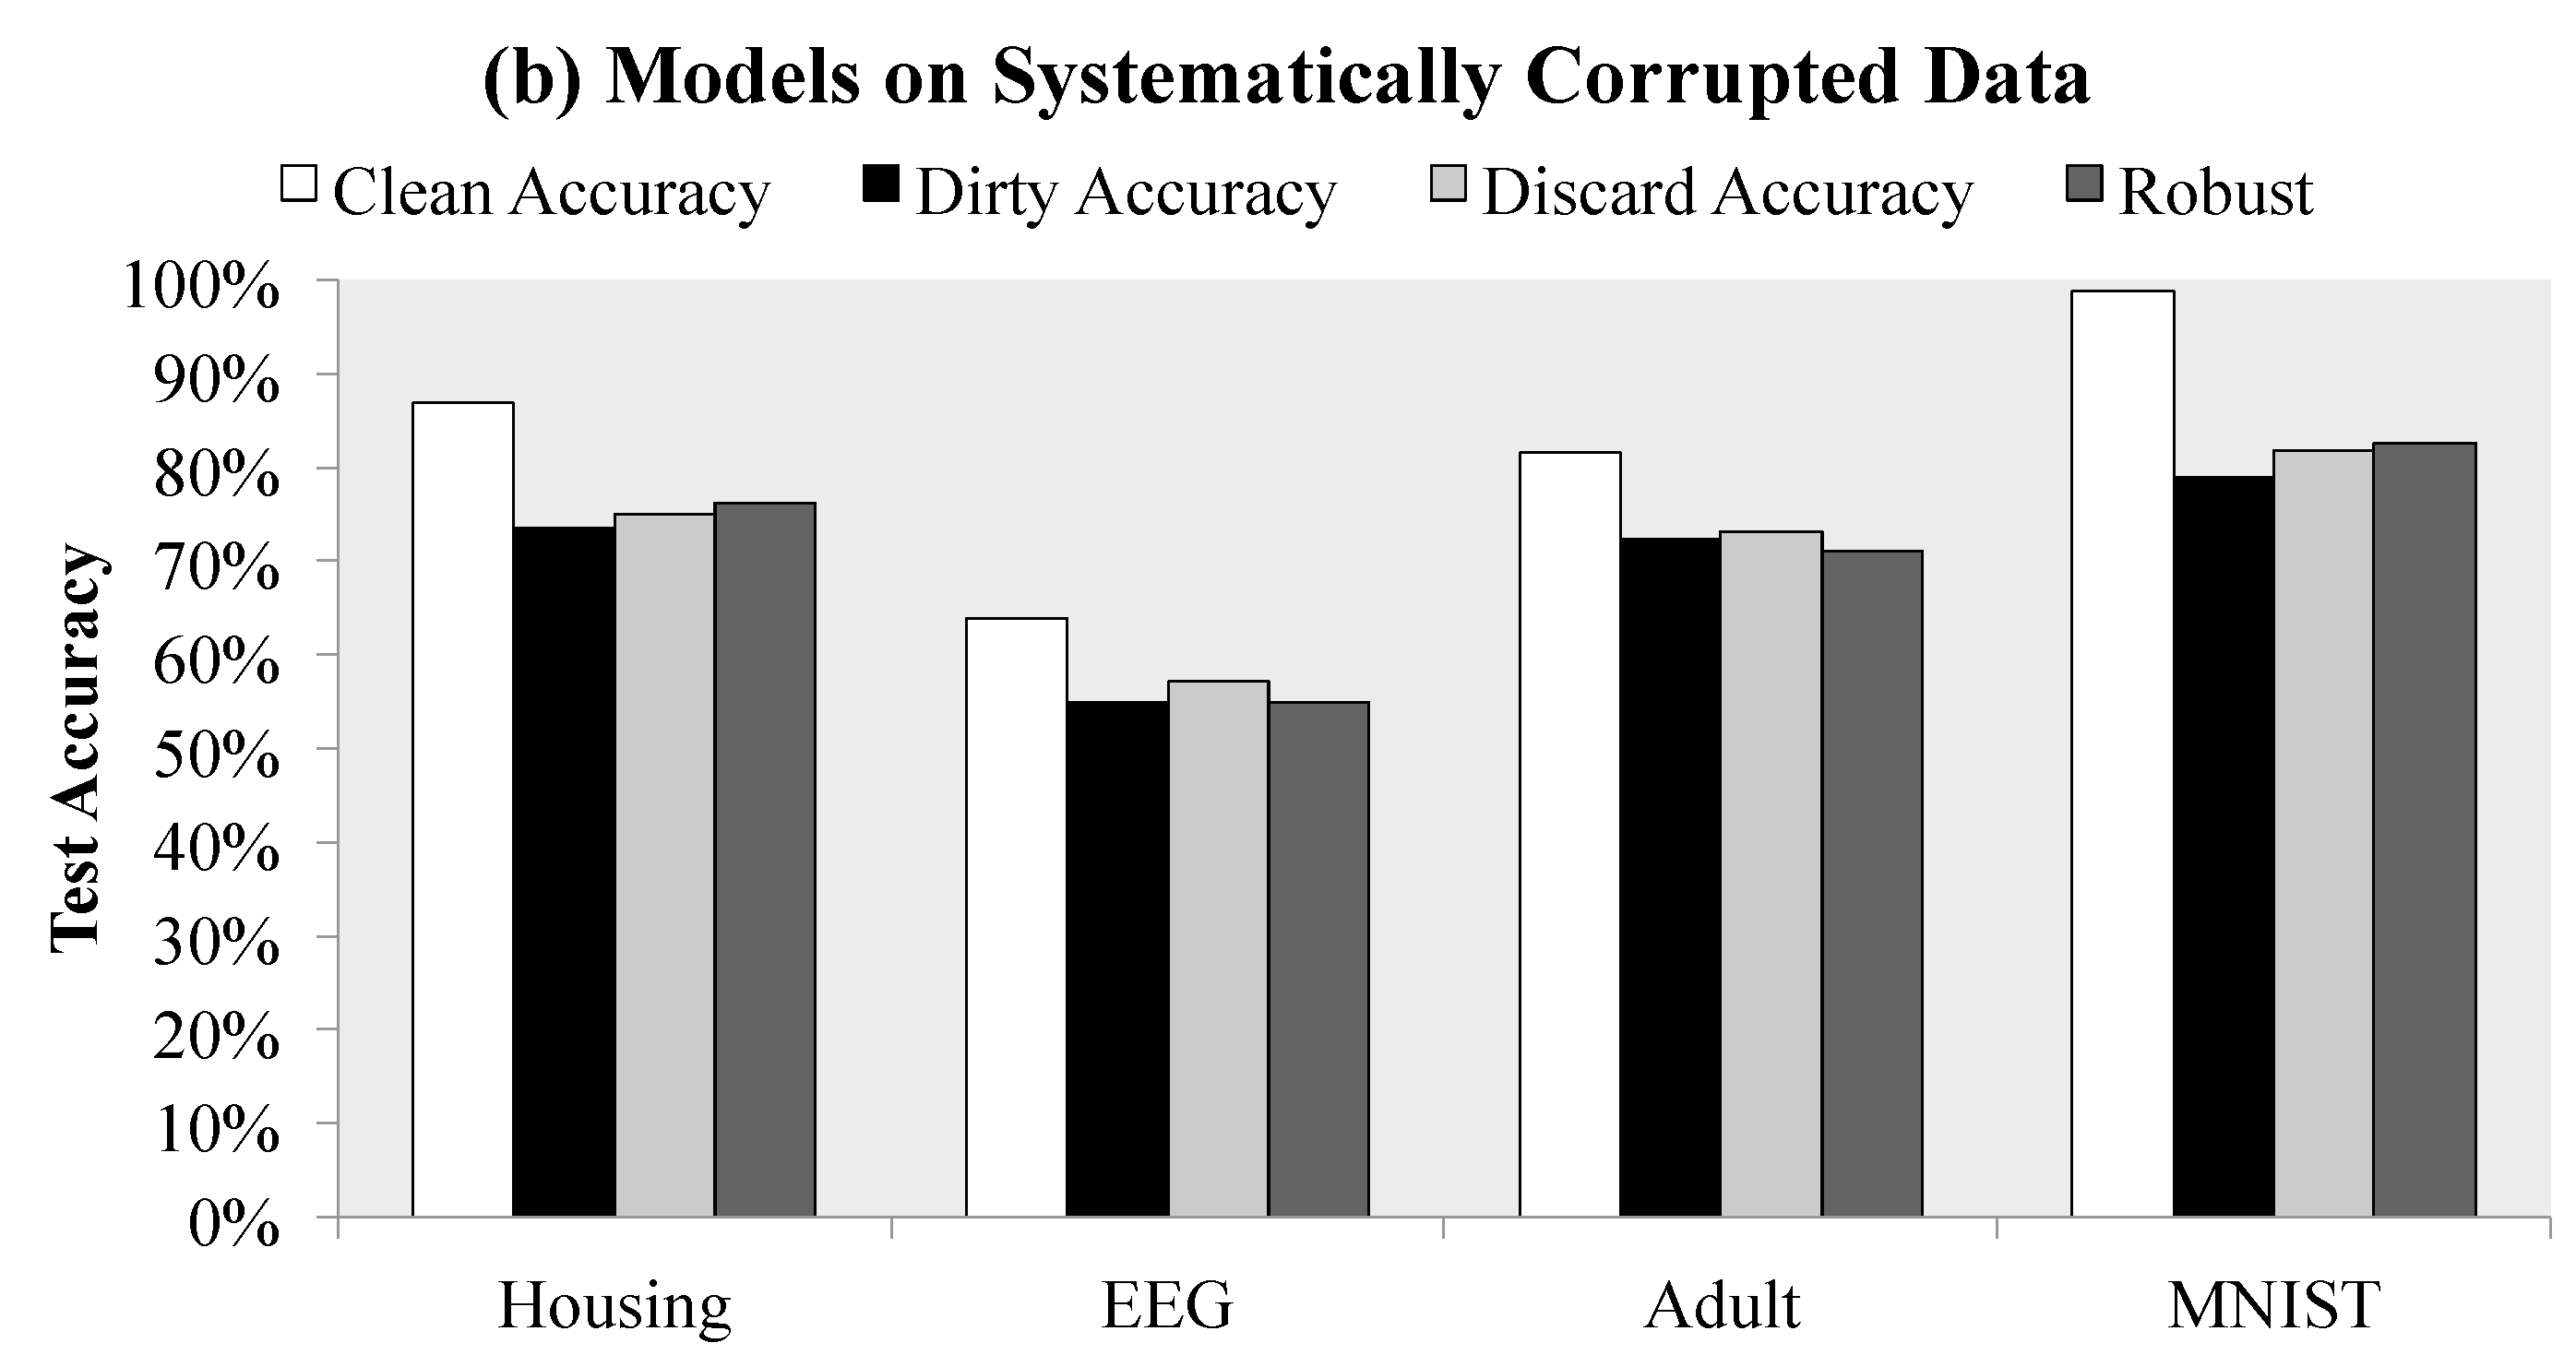
\includegraphics[width=0.8\columnwidth]{exp/exp1.pdf}
 \caption{Robust techniques work best when corrupted data are random and look atypical. Data cleaning can provide reliable performance in both the systematically corrupted setting and randomly corrupted setting.\label{sys-rand}}
\end{figure}

In Figure \ref{sys-rand}, we present the results of this experiment.
As we argued in this paper, the robust method performs well on the random high-magnitude outliers, however, falters on the systematic corruption.
Interestingly enough, in the random setting, discarding dirty data also performs well.
However, when errors are systematic data cleaning is the most reliable option across datasets.
In the MNIST dataset, we see a particularly significant effect of systematic corruption
where the test accuracy drops from nearly 98\% to 78\%.
Multiclass classification is particularly sensitive to systematic corruption when the corruptions can make classes ambiguous (e.g. reconizing a ``4" and a ``9").
The problem is that a priori, we do not know if data error is random or systematic.
While data cleaning requires more effort, it provides benefits in both settings.

\subsection{Experiment 2. Prioritization}
The next set of experiments evaluate different approaches to cleaning a sample of data.
In this set of experiments, we use the random errors generated above.

\subsubsection{2a. Alternative Algorithms}
In our first prioritization experiment, we evaluate the samples-to-error tradeoff between three alternative algorithms:

\noindent\textbf{SampleClean (SC): } In SampleClean, we do not use a gradient update and instead take a sample of data and train the model to completion on the sample.

\noindent\textbf{Active Learning (AL): } In Active Learning, we do not consider the effect of ``data cleaning" and prioritze points by their dirty gradient value. We do, however, do this iteratively and update the model.

\noindent\textbf{ActiveClean Oracle (AC+O): } In ActiveClean Oracle, we importance sample points by their clean gradient. This represents the theoretical best that our algorithm could hope to achieve given perfect error estimation.

In Figure \ref{prio-perf}, we present our results on Housing, Adult, and EEG. 
We find that \sys gives its largest benefits for small sample sizes (up-to 12x).
\sys makes significant progress because of its intelligent initialization, iterative updates, and partitioning.
For example, the EEG dataset is the hardest classification task.
SampleClean has difficulty on this dataset since it takes a uniform sample of data (only 5\% of which are corrupted on average) and tries to train a model using only this data.
\sys and Active Learning leverage the initialization from the dirty data to get an improved result. 
However, \sys's impact estimates and error partitioning allow us to beat Active Learning on all three of the datasets.

\begin{figure*}[t]
\centering
 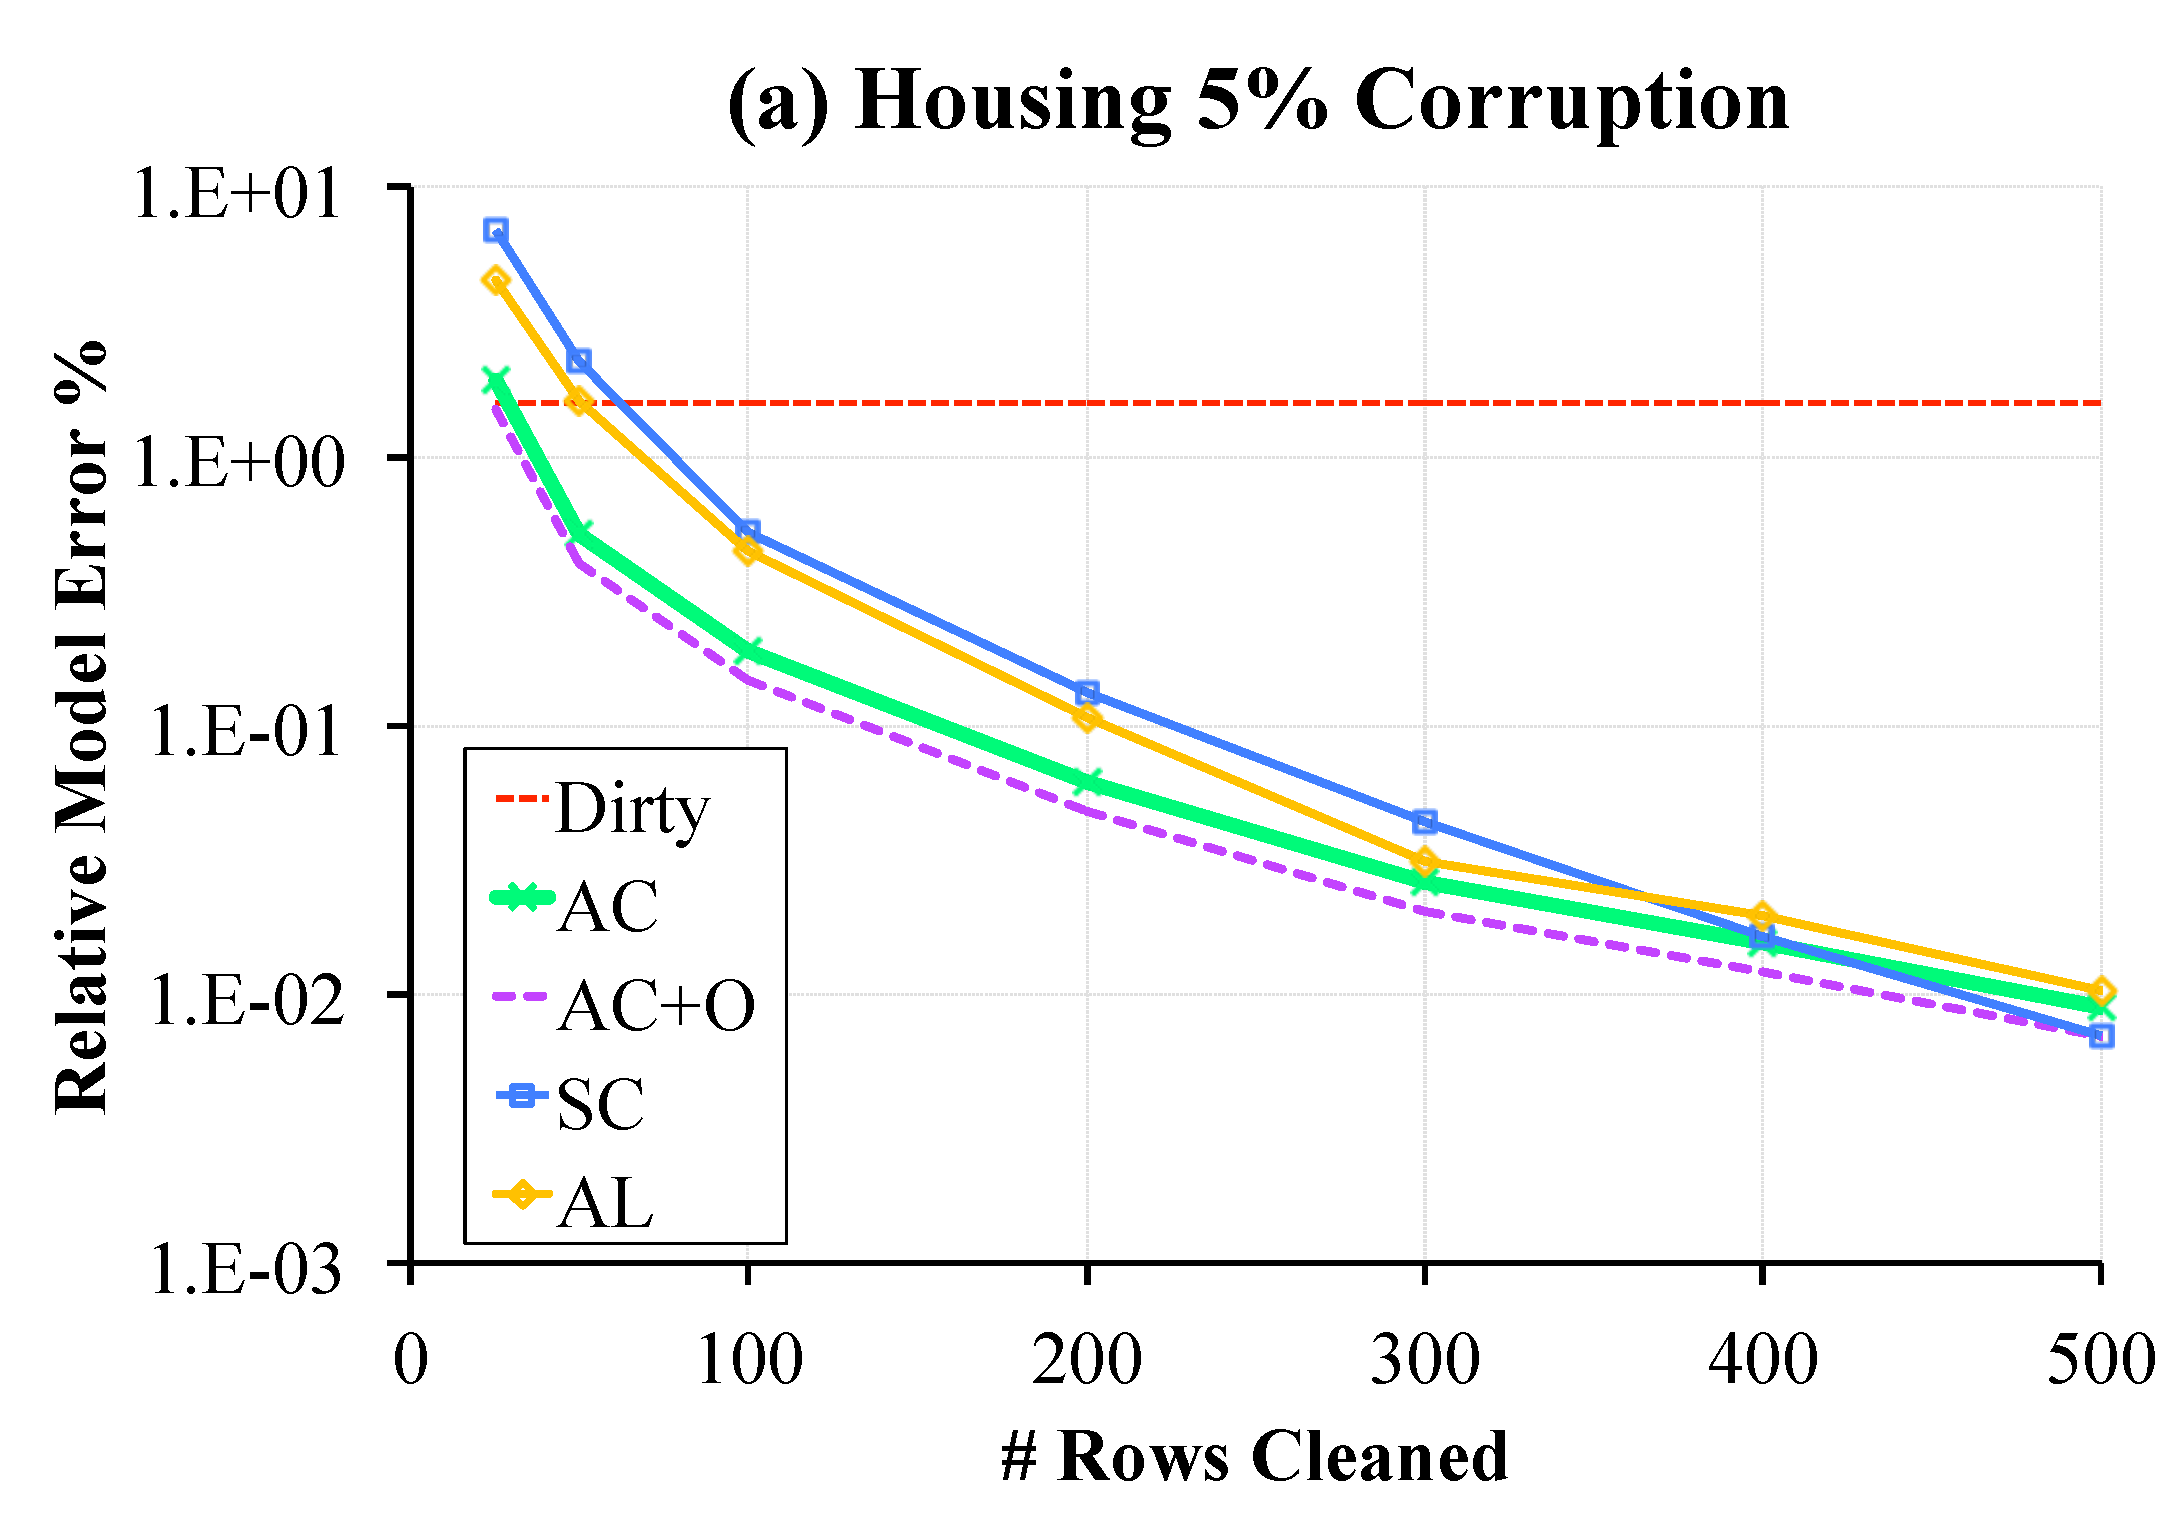
\includegraphics[scale=0.15]{exp/exp3a.pdf}
 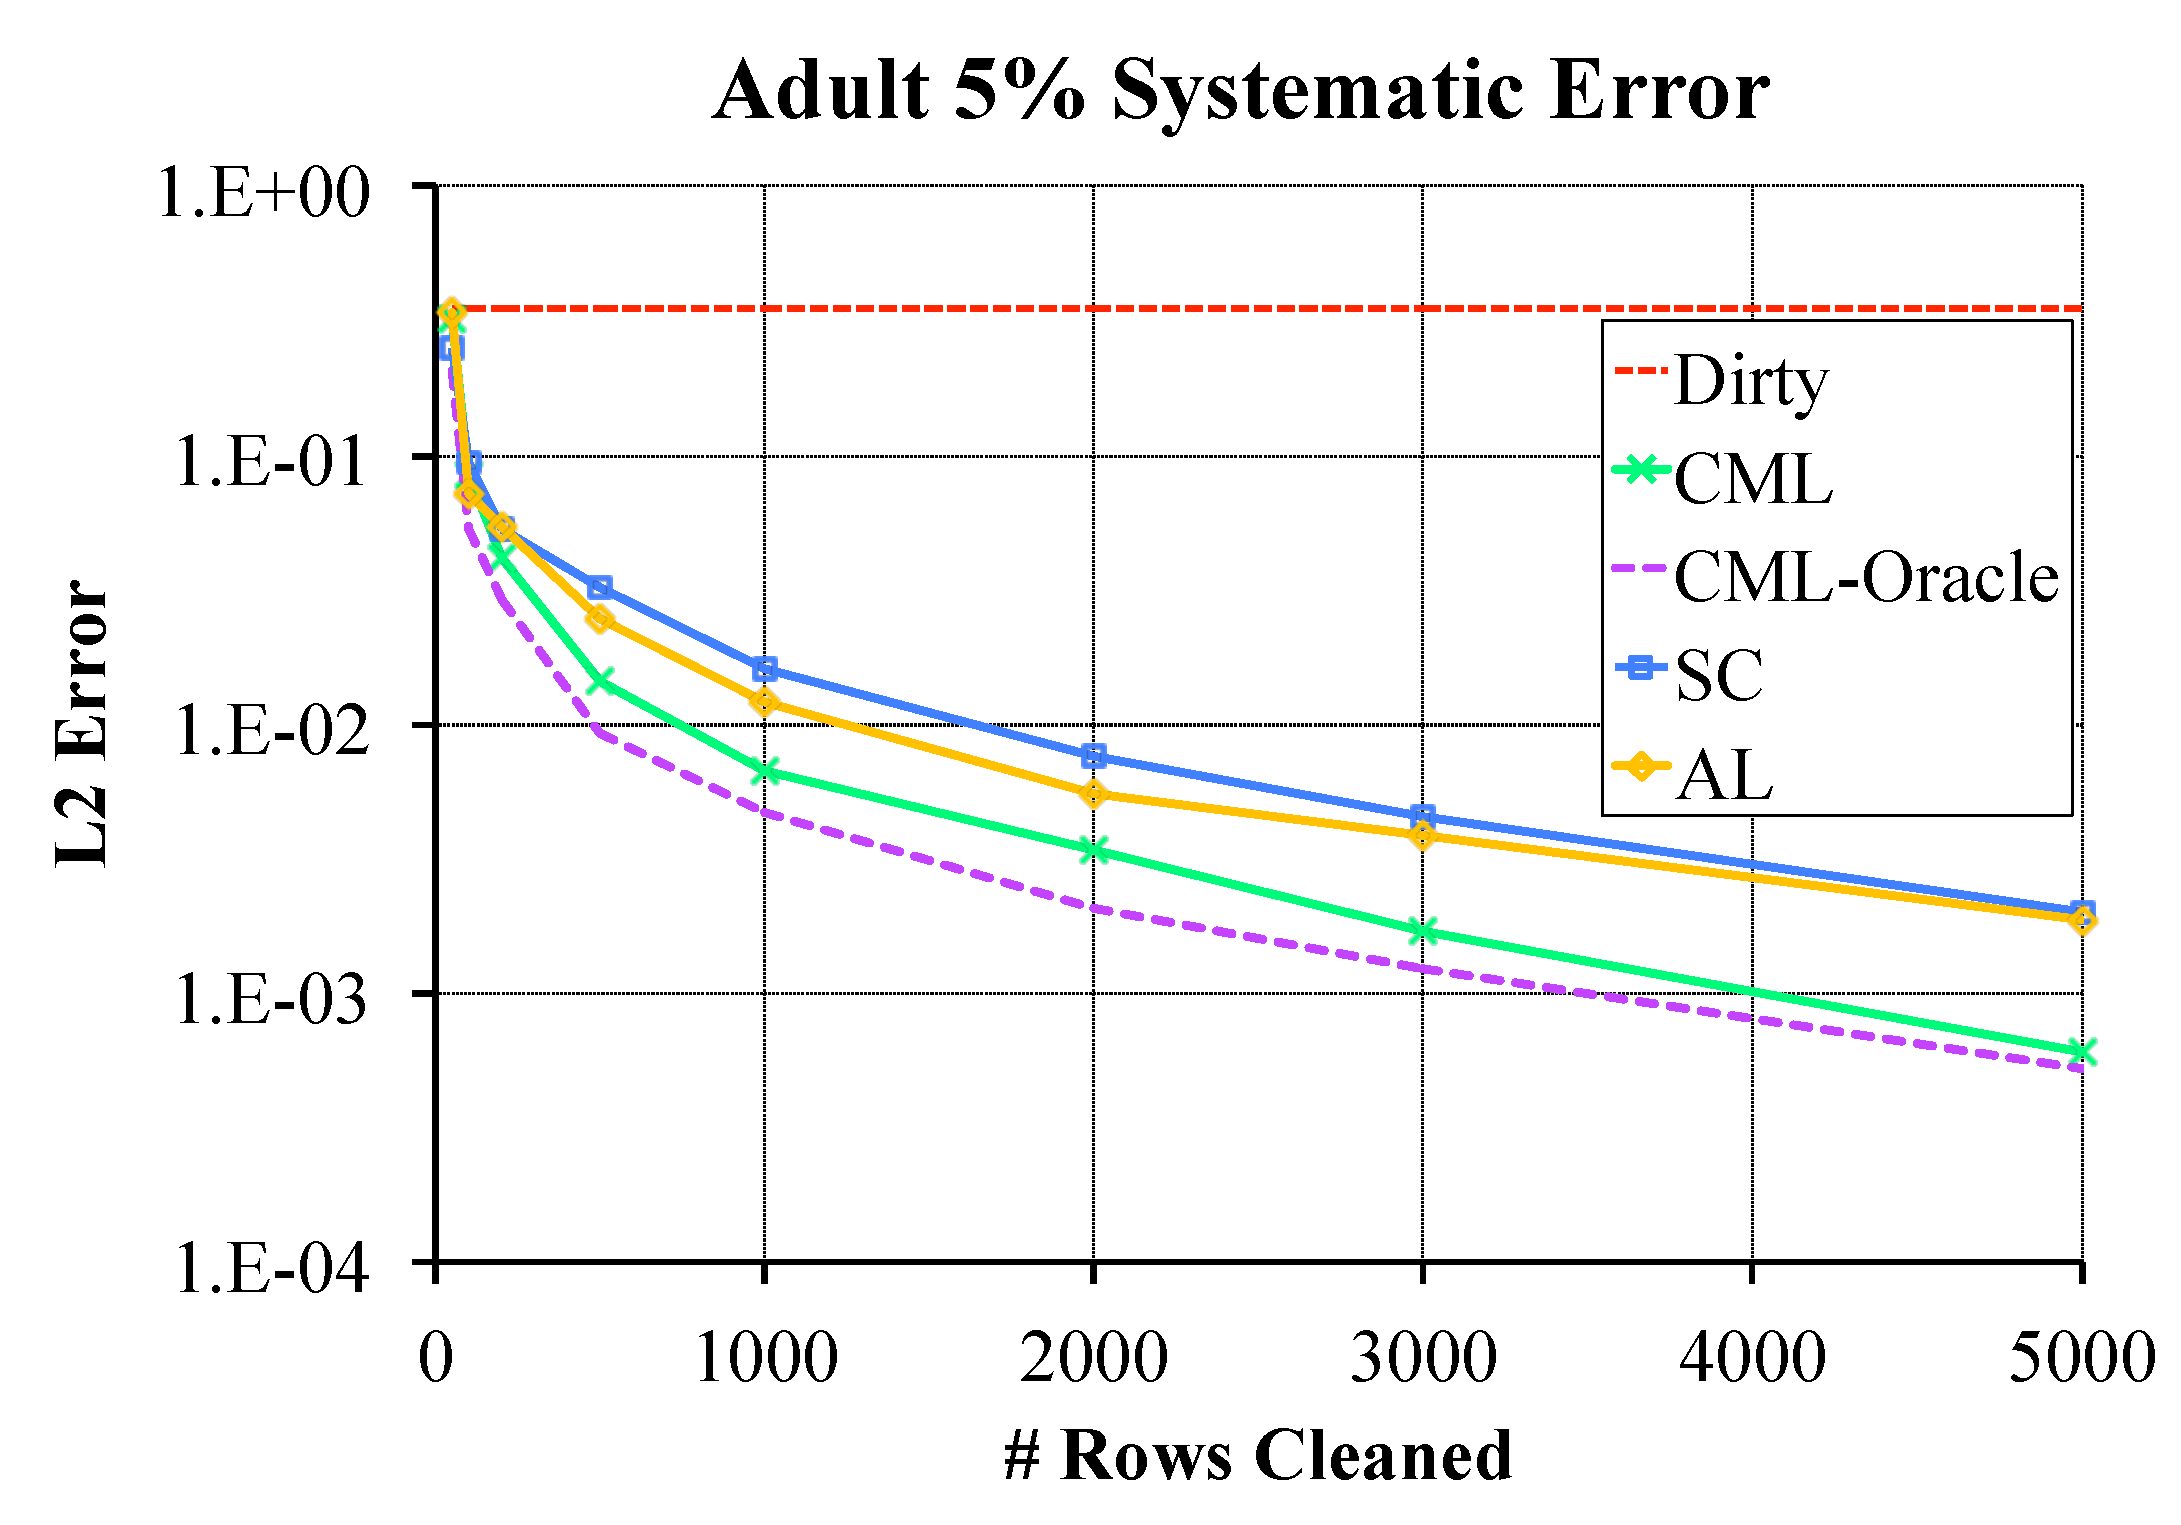
\includegraphics[scale=0.15]{exp/exp3b.pdf}
  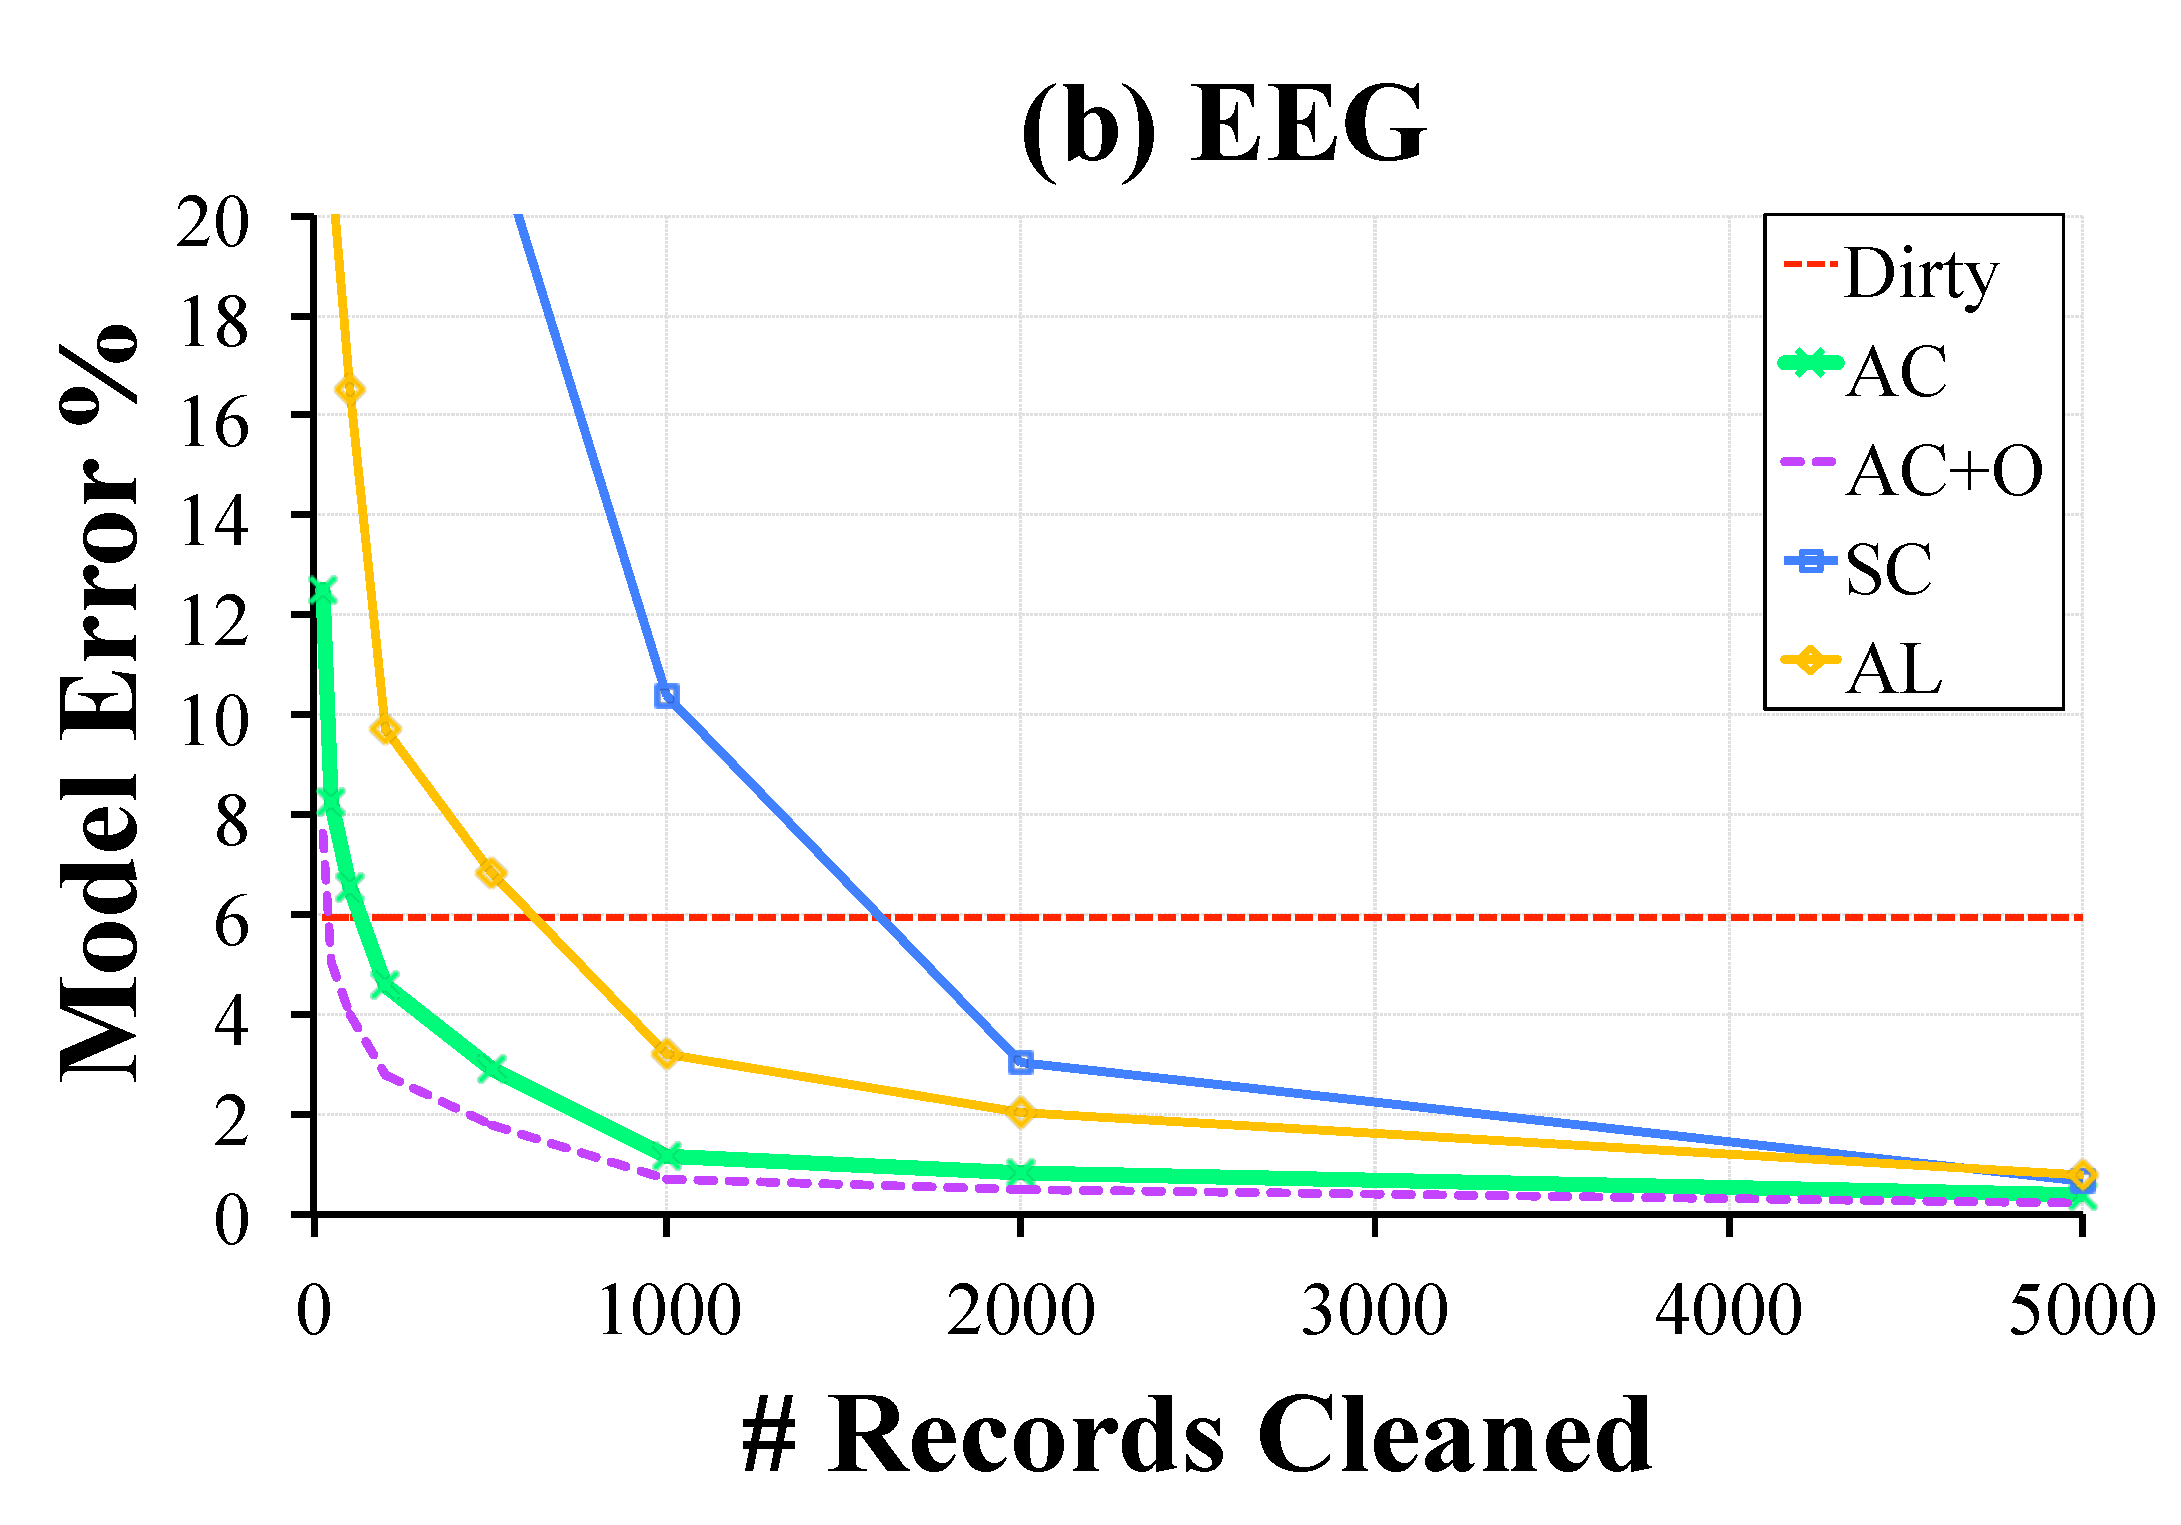
\includegraphics[scale=0.15]{exp/exp3c.pdf}
 \caption{\sys converges with a smaller sample size to the true result in comparison to Active Learning and SampleClean. \label{prio-perf}}
\end{figure*}

\subsubsection{2b. Source of Improvements}
Throughout the paper, we proposed numerous optimizations.
Now, we try to understand the source of our improvements w.r.t Active Learning and SampleClean.
We pick a single point on the curves shown in Figure \ref{prio-perf} that corresponds to 10\% of the data cleaned (55 for Housing, 4555 for Adult, 150 for EEG) and compare the performance of \sys with and without various optimizations.
We denote \sys without partitioning as (AC-P) and \sys without partitioning and importance sampling as (AC-P-I).
In Figure \ref{opts}, we plot the relative error of the alternatives w.r.t to the optimized version of \sys.
Partitioning significantly improves our results in all of the datasets, and accounts for a substantial part of the improvements over Active Learning.
However, when we remove partitioning we still see some improvements since our importance sampling relies on error impact estimates that judge how valuable a point is to the clean model rather than the dirty model in Active Learning.
Not surprisingly, when we remove both these optimizations, \sys is comparable or slightly worse than Active Learning.

\begin{figure}[ht!]
\centering
 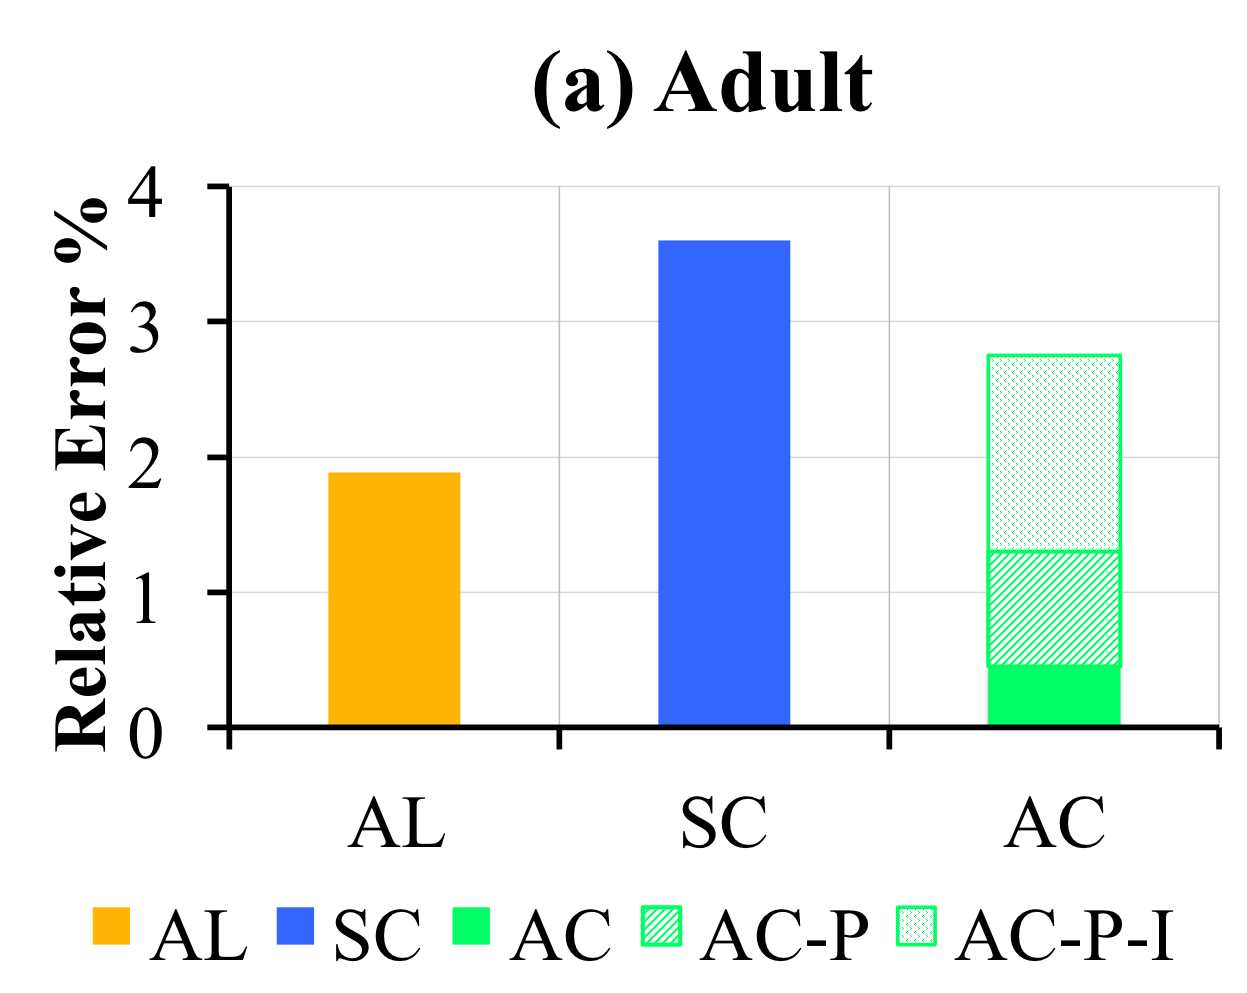
\includegraphics[width=\columnwidth]{exp/exp8.png}
 \caption{We clean 10\% of the data with the alternative algorithms and also include variants of \sys with optimization removed. We plot the relative error w.r.t the optimized \sys. Both partitioning and importance sampling lead to significant reductions in error. \label{opts}}
\end{figure}

We evalue Active Learning and \sys to better understand this relationship.
In Figure \ref{albias}, we vary the biasing effect of our random corruptions.
That is, we start with zero mean noise and increase the mean value and variance of the noise.
Since Active Learning uses the gradient, if there is zero mean noise, in expectation, the dirty data and clean data are the same.
However, as the bias increases, the fact that Active Learning prioritizes w.r.t to the dirty data matters more and becomes increasingly erroneous w.r.t to \sys.

\begin{figure}[ht!]
\centering
 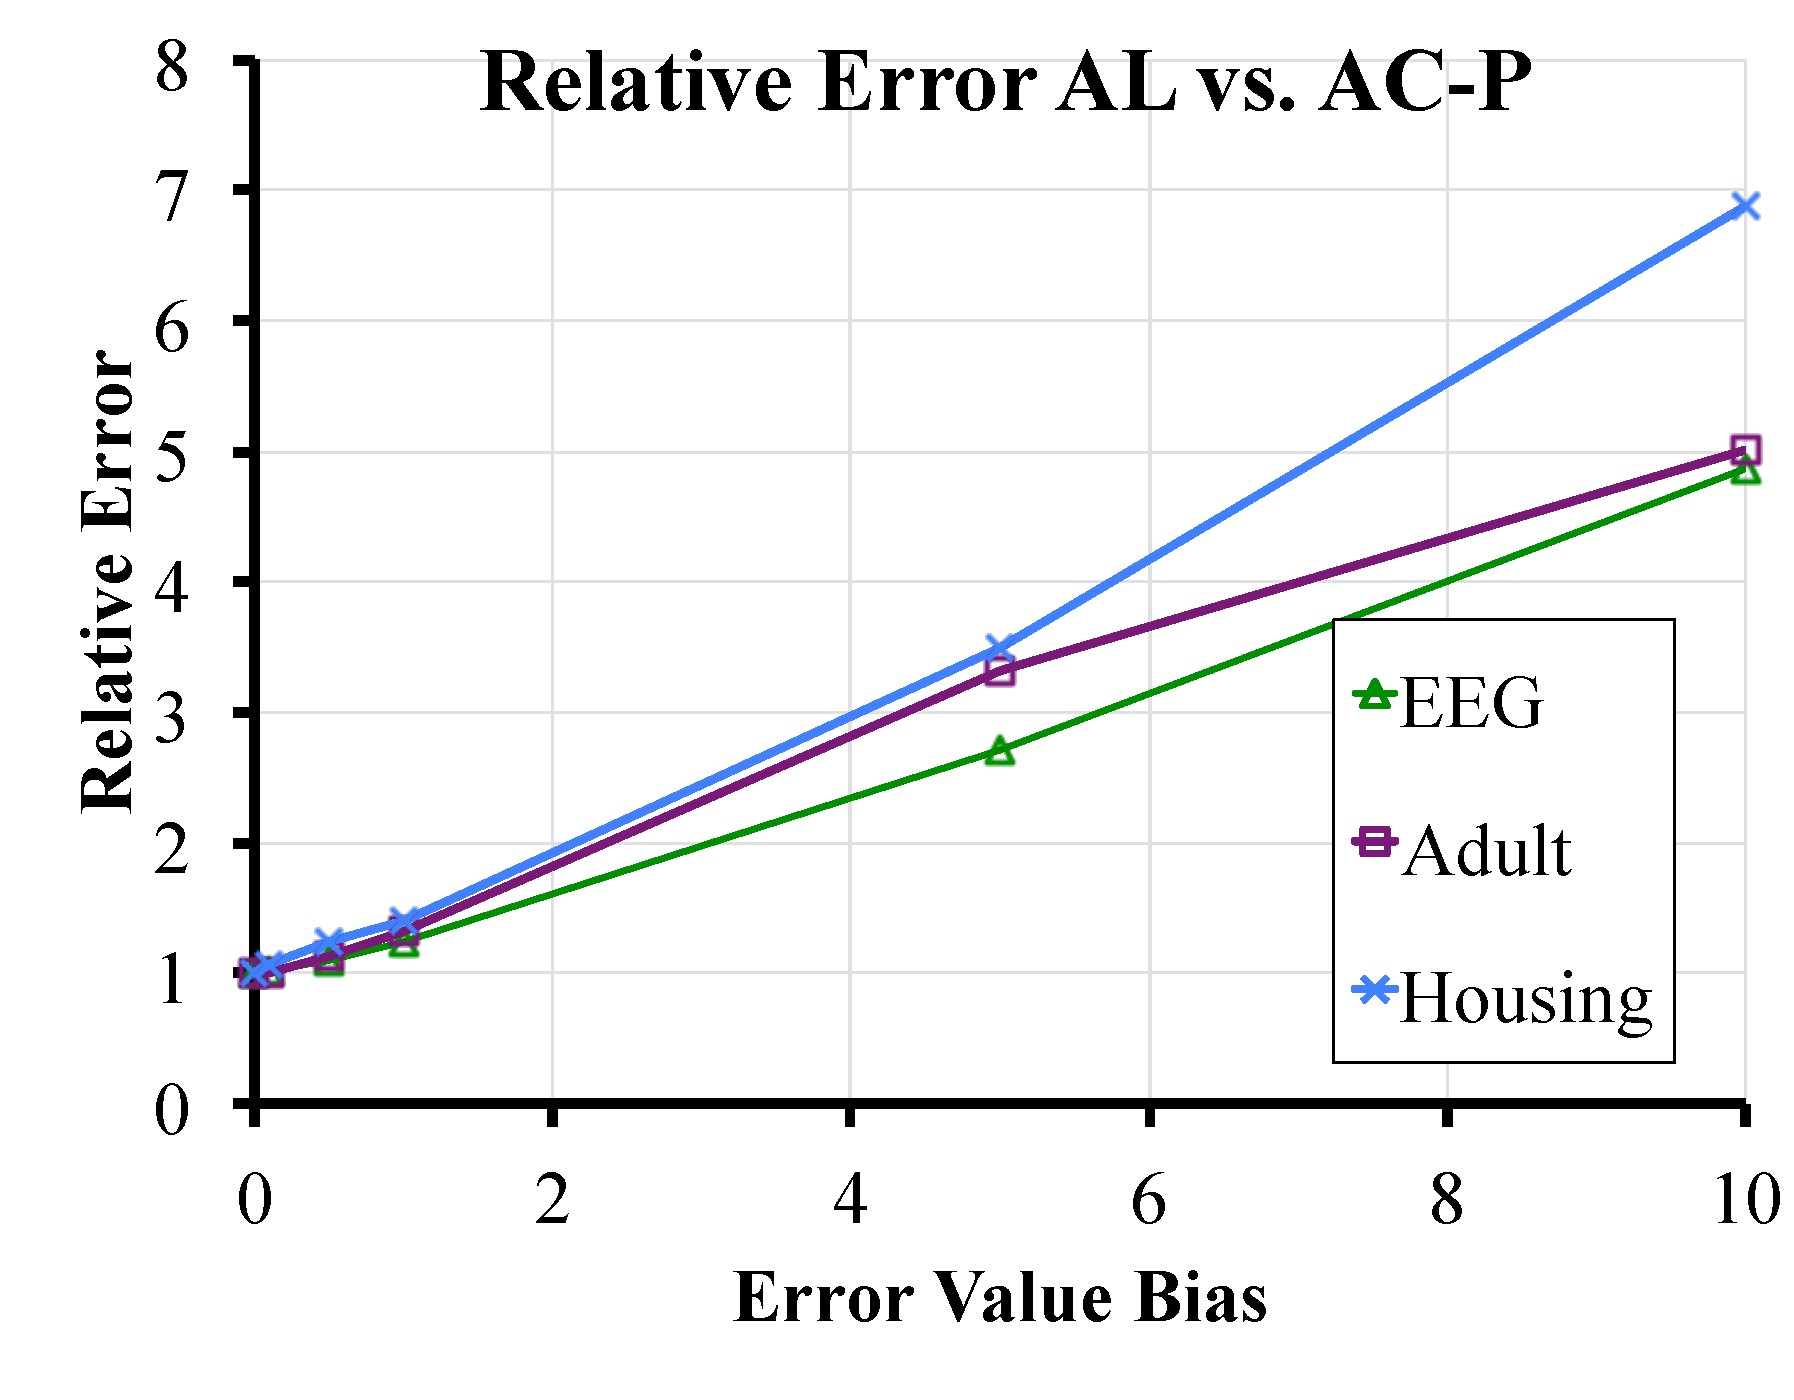
\includegraphics[width=0.6\columnwidth]{exp/exp10.pdf}
 \caption{As we increase the biasing nature of the corruption, Active Learning is increasingly erroneous w.r.t \sys. \label{albias}}
\end{figure}

\subsubsection{2c. Error Dependence}
Both Active Learning and \sys outperform SampleClean in our experiments.
In our next experiment, we try to understand how much of this performance 
is due to the initialization (i.e., SampleClean trains a model from ``scratch").
We vary the rate of random error, thus making the initialization more and more arbitrary, 
and measure the relative performance between SampleClean and \sys.
Since SampleClean only acts on a clean sample of data, it is robust to data error.
So at some point, the errors in the data are so significant that training a model on a small but clean sample of data is more efficient than iteratively updating the dirty model.

In Figure \ref{bias}, we present the results from this experiment.
We corrupt entries from the data matrix of the Adult dataset at random (probability on plotted on the x-axis).
Then, we measure the number of records we need to clean before we have a relative error of 0.1\%.
We find that at about 30\% corruption rate, SampleClean is more accurate than \sys.
Since the Adult dataset has 12 features, a 30\% corruption rate corresponds to each example with 3.6 features incorrect on average.
We optimized \sys for sparse and relatively small errors but it still shows reasonable performance even in this highly erroneous setting. 
At higher corruption rates, \sys requires more than one epoch to converge to an accurate answer which requires cleaning almost all of the data.

\begin{figure}[ht!]
\centering
 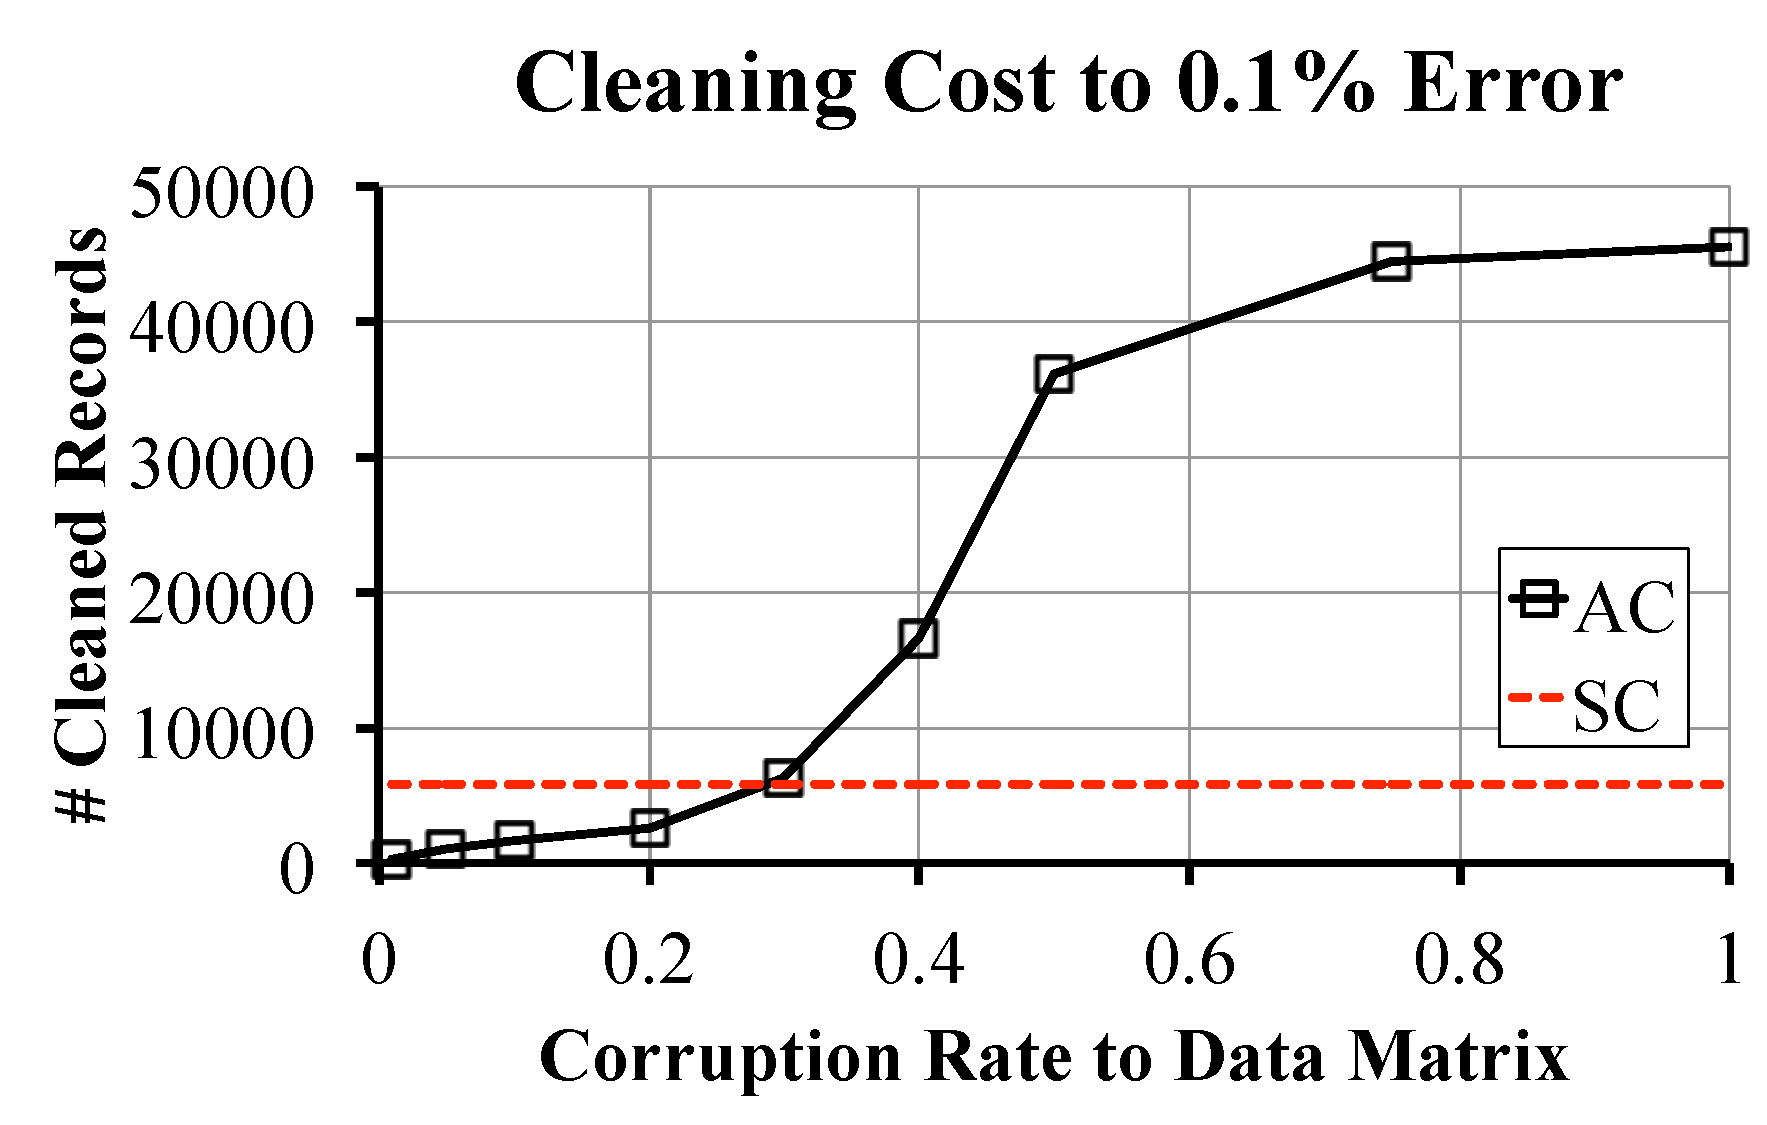
\includegraphics[width=0.6\columnwidth]{exp/exp9.pdf}
 \caption{We corrupt an increasing number of entries in the data matrix. At about 30\% corrupted, \sys is no longer more efficient than SampleClean. \label{bias}}
\end{figure}

\subsubsection{2d. Testing Accuracy}
In the previous experiments, we studied the relative model error which measures the training loss. 
However, to an end user the metric that matters is test accuracy.
In the next experiment, we try to understand how reductions in model error correlate to improvements in test error.
In Figure \ref{prio-tperf}, we present the results for the three datasets: Adult, Housing, and EEG.
We find that in two of the datasets, Housing and Adult, \sys converges to clean test accuracy faster than the alternatives.

However, there is a curious negative result with the EEG dataset that we would like to highlight. 
We find that even though \sys has significantly lower model error (Figure \ref{prio-perf}), this does not correspond to as significant of an increase in test accuracy.
We speculate this is due to the inherrent hardness of the EEG classification problem.
\sys may encourage overfitting at intermediate results for hard classification tasks.
The solution to this problem may be to add additional regularization, thus actually changing the optimization problem.
We hope to explore this problem in further detail in future work.

\begin{figure*}[t]
\centering
 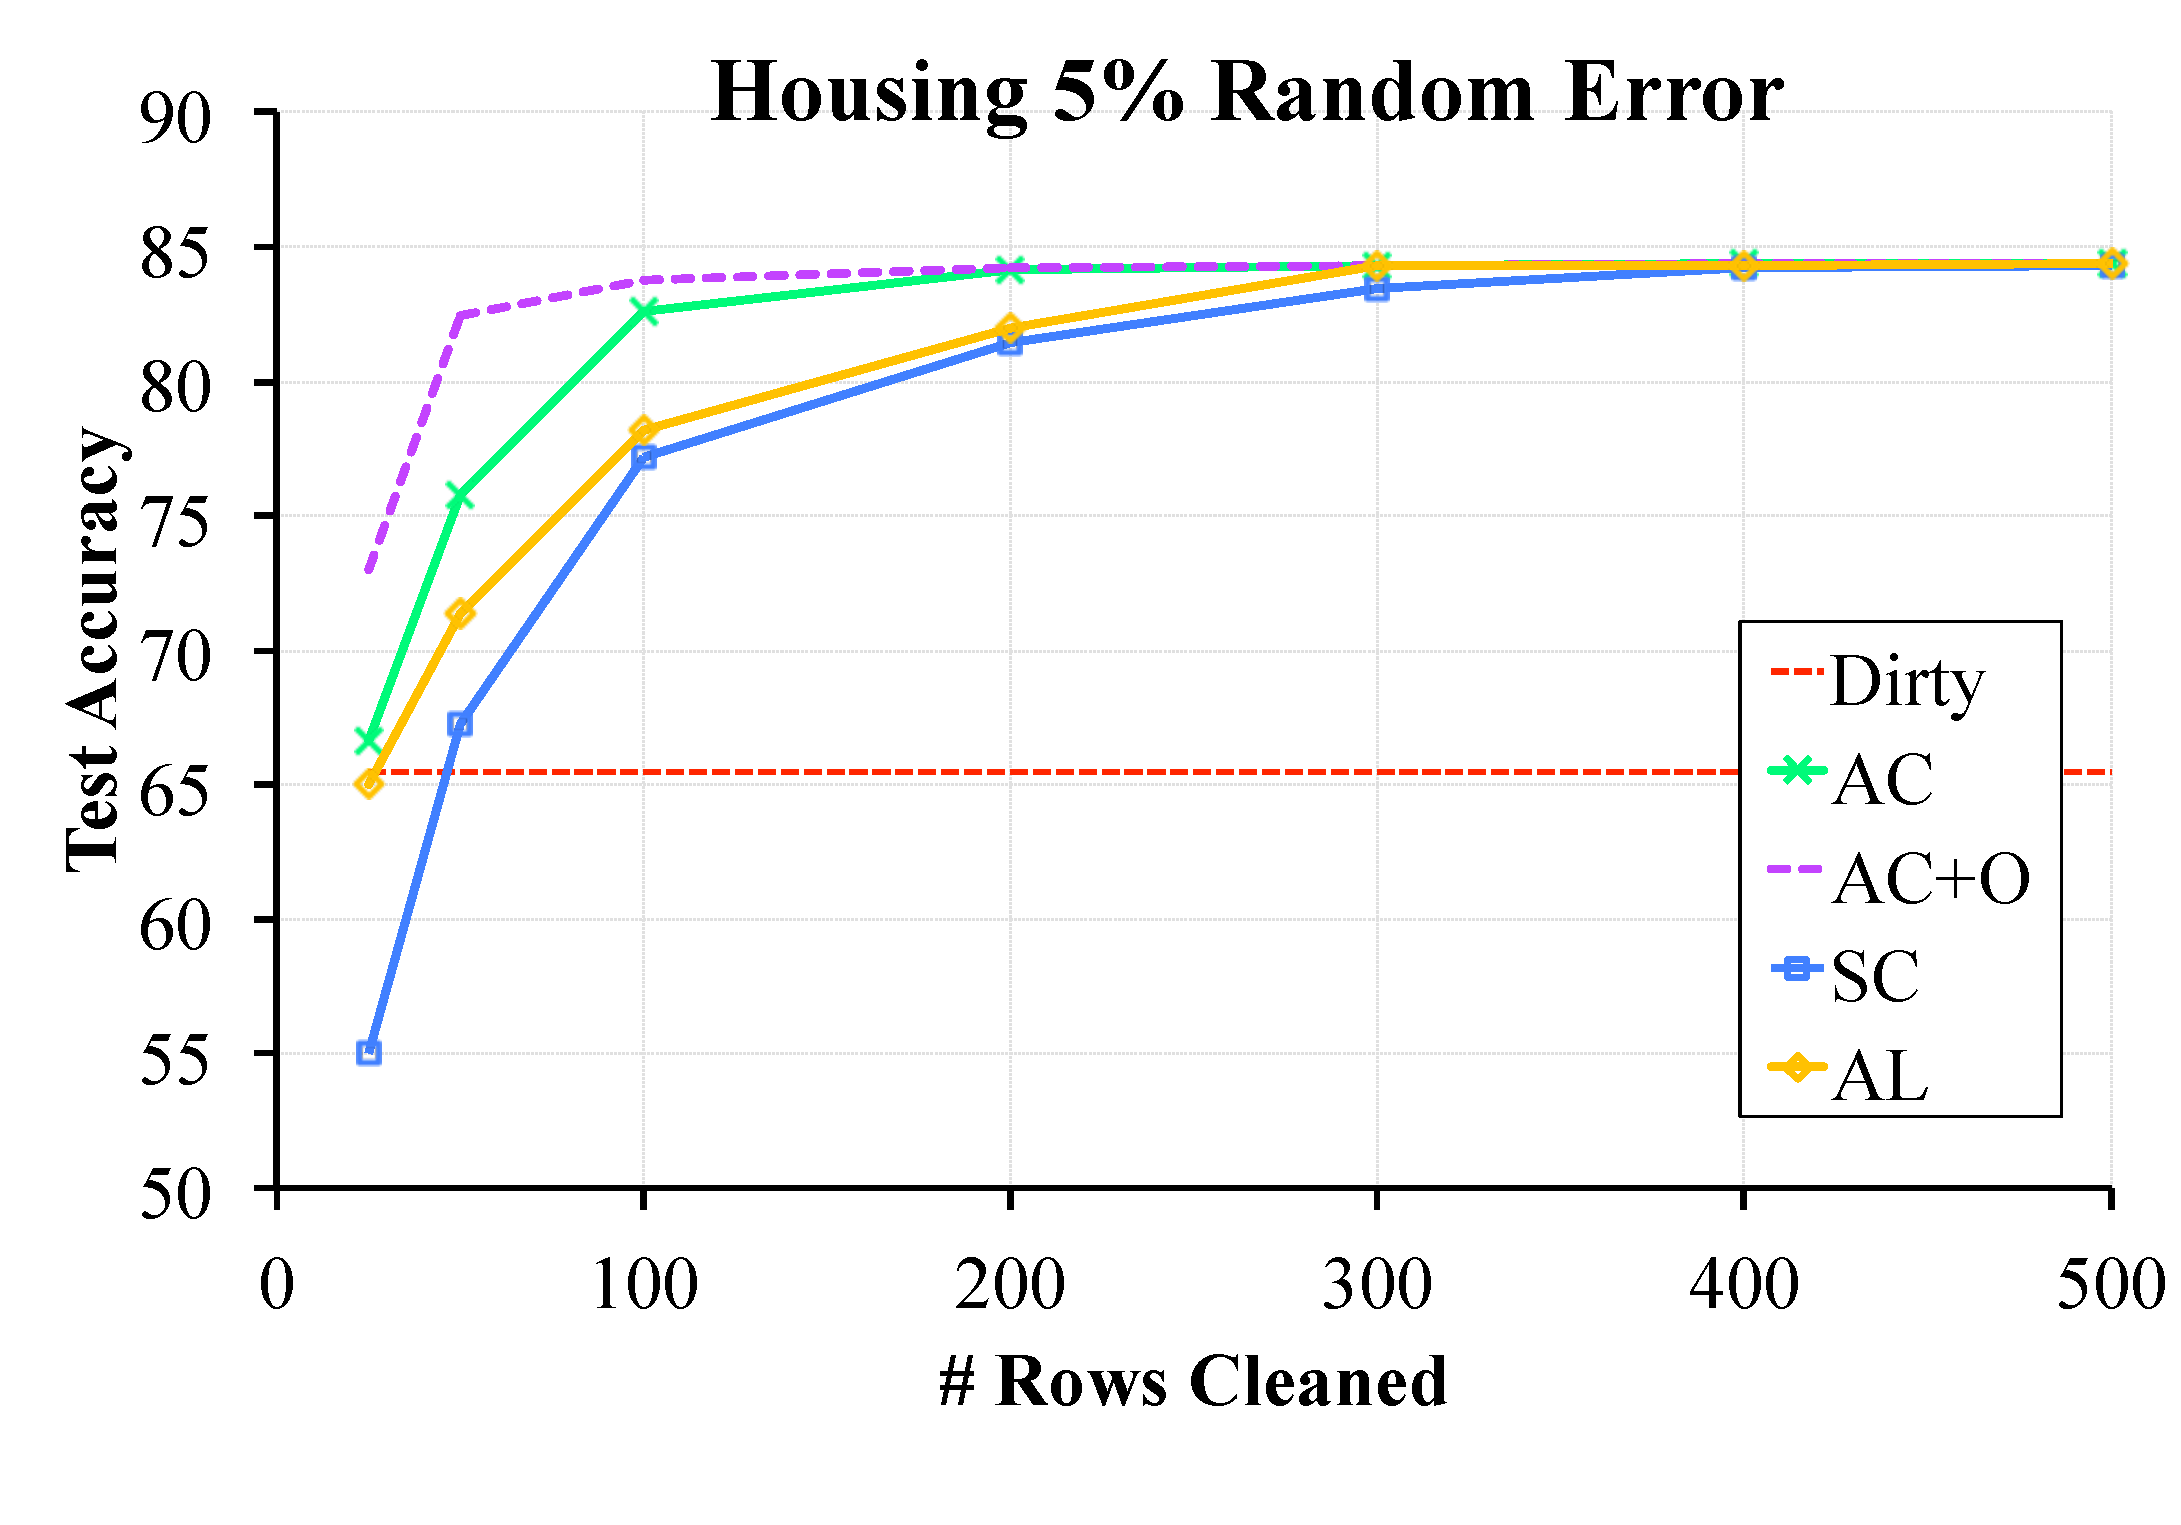
\includegraphics[scale=0.15]{exp/exp3aa.pdf}
 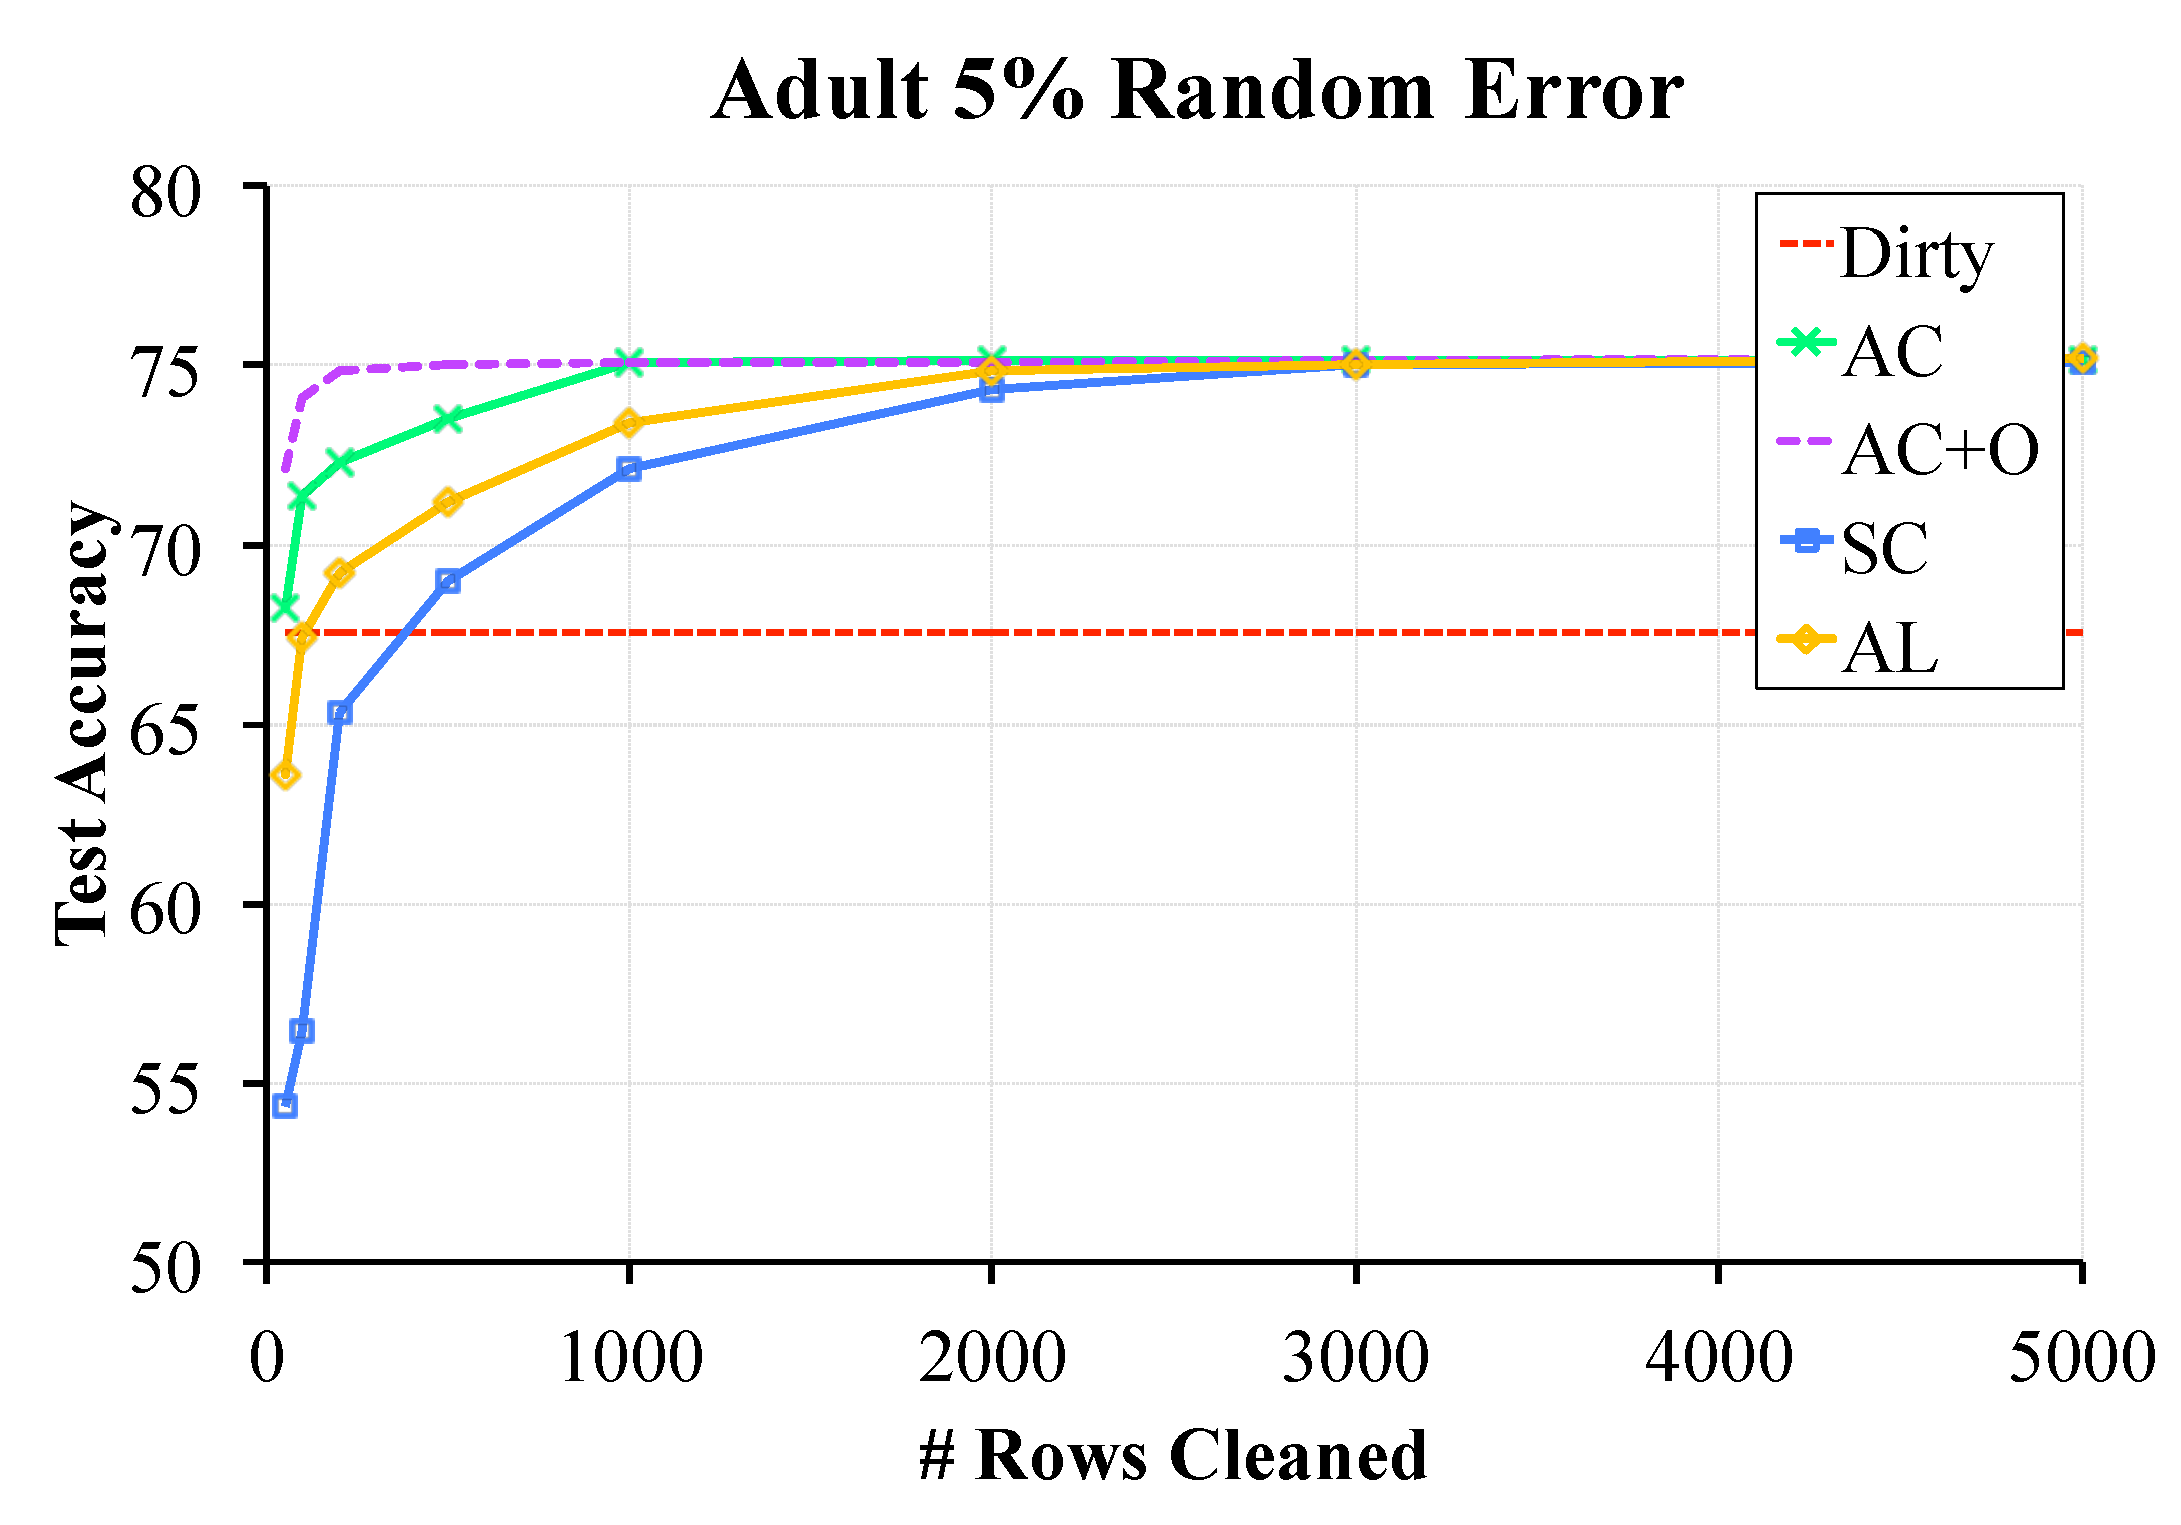
\includegraphics[scale=0.15]{exp/exp3bb.pdf}
  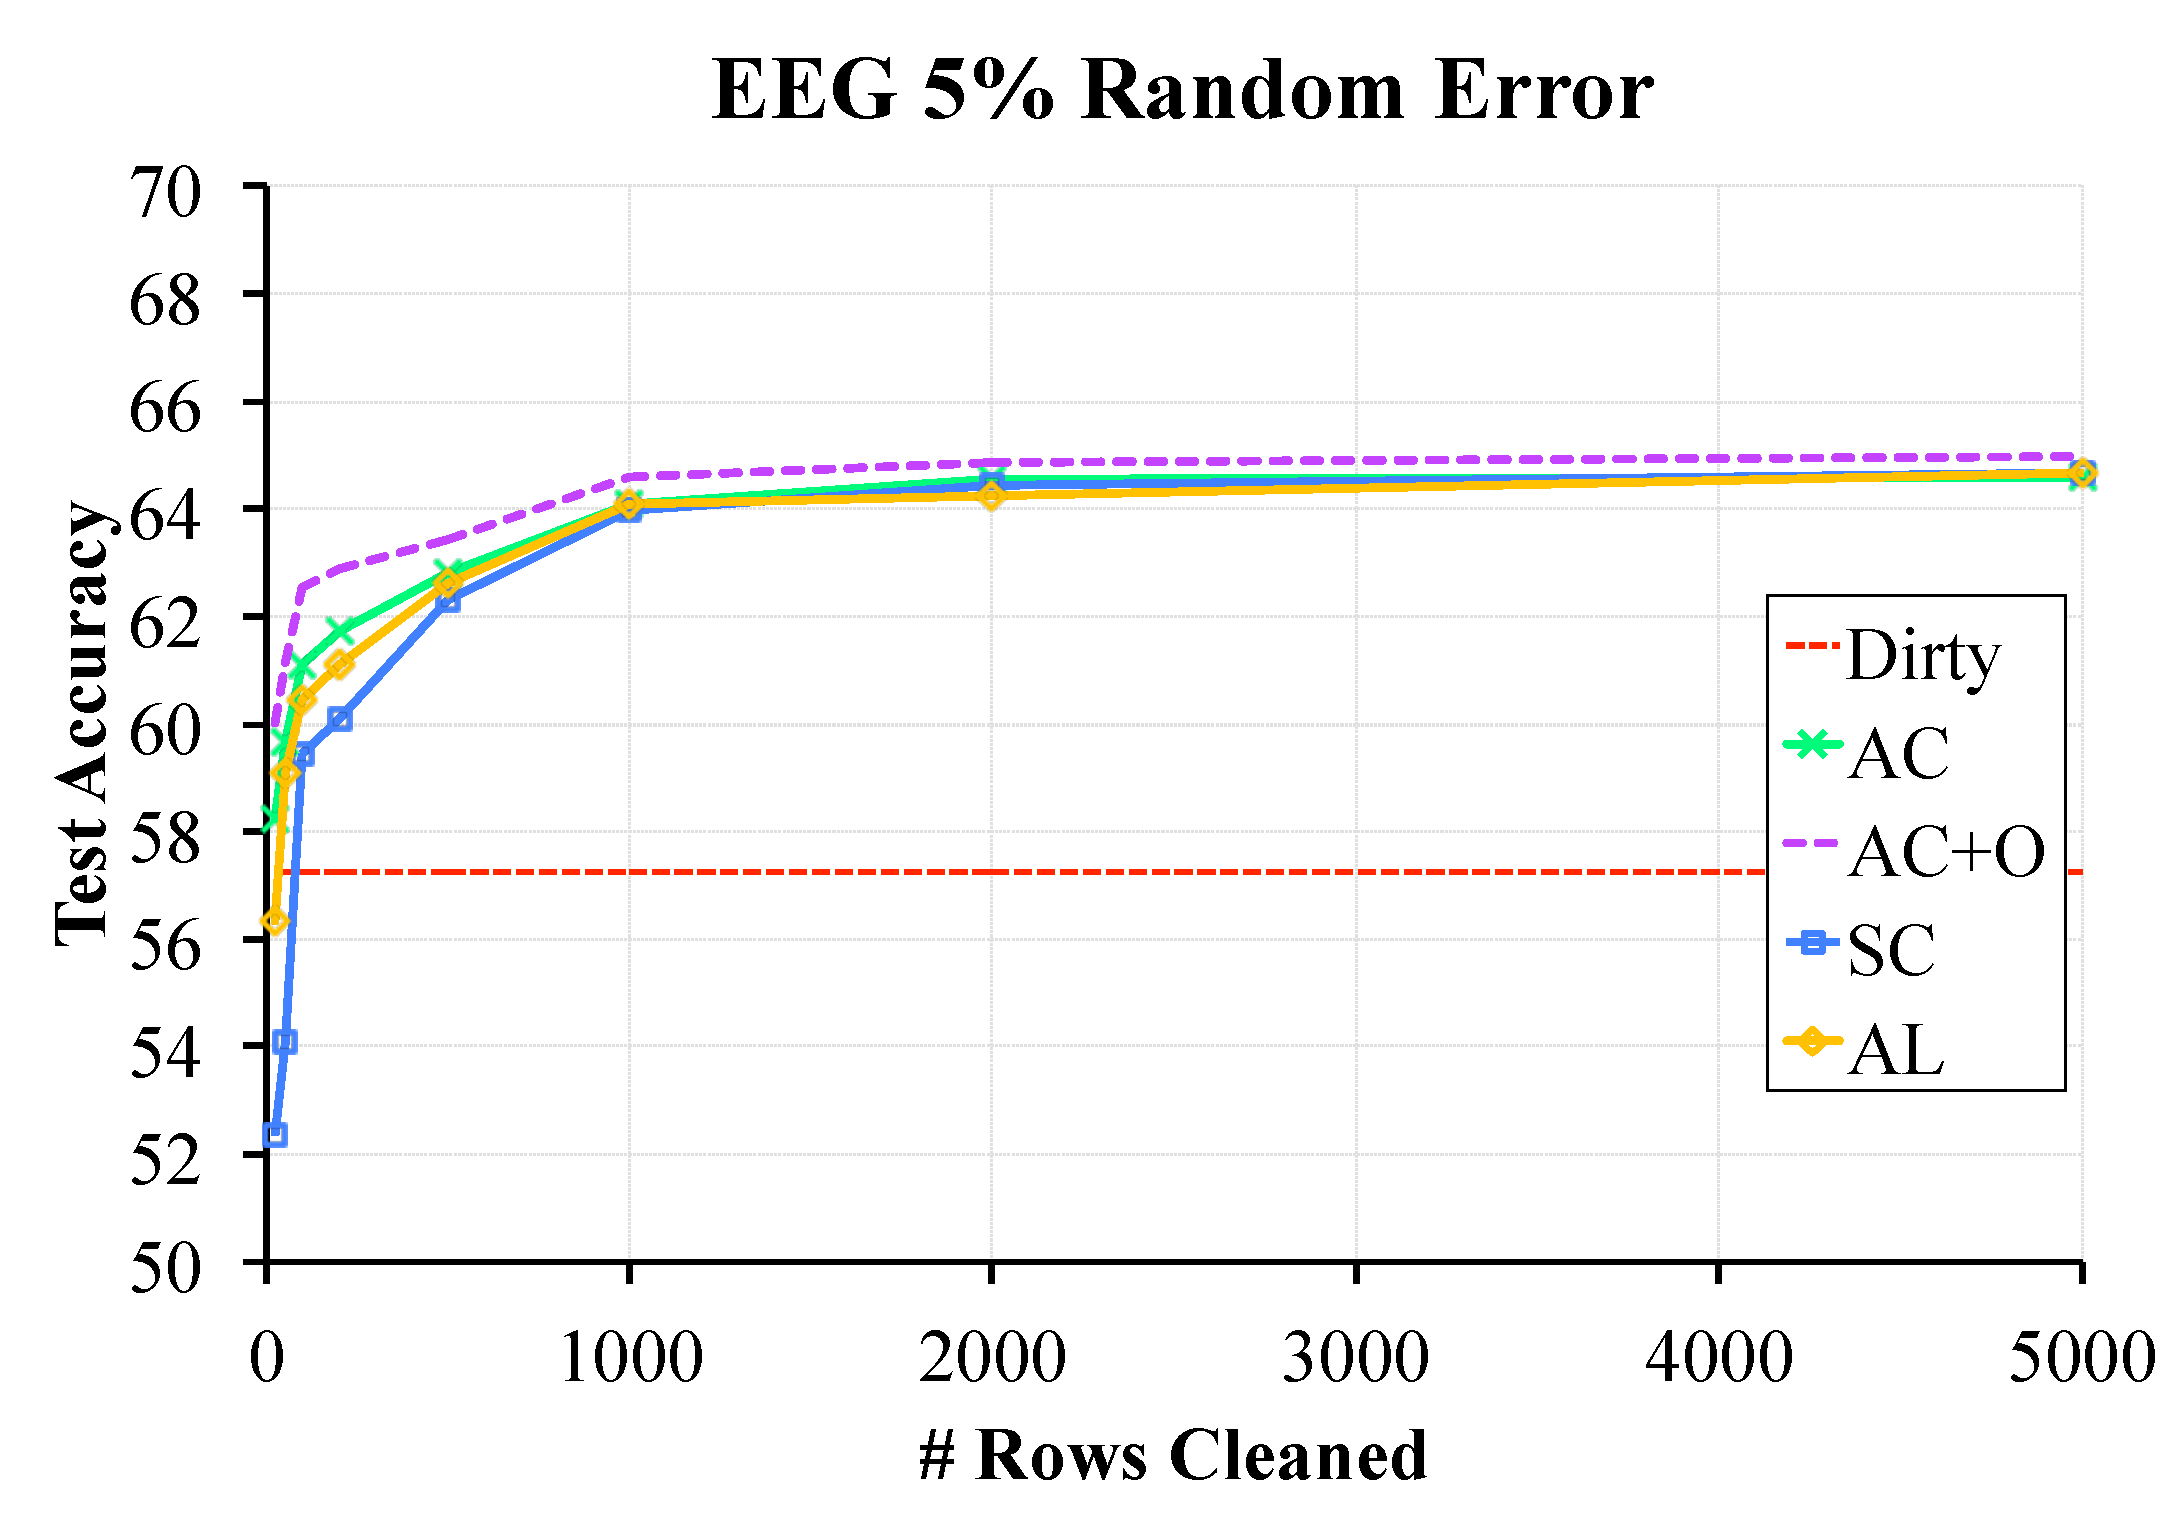
\includegraphics[scale=0.15]{exp/exp3cc.pdf}
 \caption{\sys converges with a smaller sample size to the maximum test accuracy in comparison to Active Learning and SampleClean. \label{prio-tperf}}
\end{figure*}

\subsection{Experiment 3. Predicates vs. Classification}

\subsubsection{3a. Basic Performance}
In the next set of experiments, we explore the error partitioning in more detail.
We presented two models for error sampling, one where we are given a set of candidate dirty records through a predicate and one where we have to learn this predicate as we clean.
In Figure \ref{pred-perf}, we overlay the convergence plots in the previous experiments with a curve (denoted by AC+C) that represents \sys using a classifier instead of an error predicate.
We use an SVM classifier to predict errors.
We find an interesting tradeoff where initially \sys is comparable to Active Learning (explanation for why seen in Figure \ref{opts}), as our classifier becomes more effective the partitioning improves the performance.

\begin{figure}[t]
\centering
 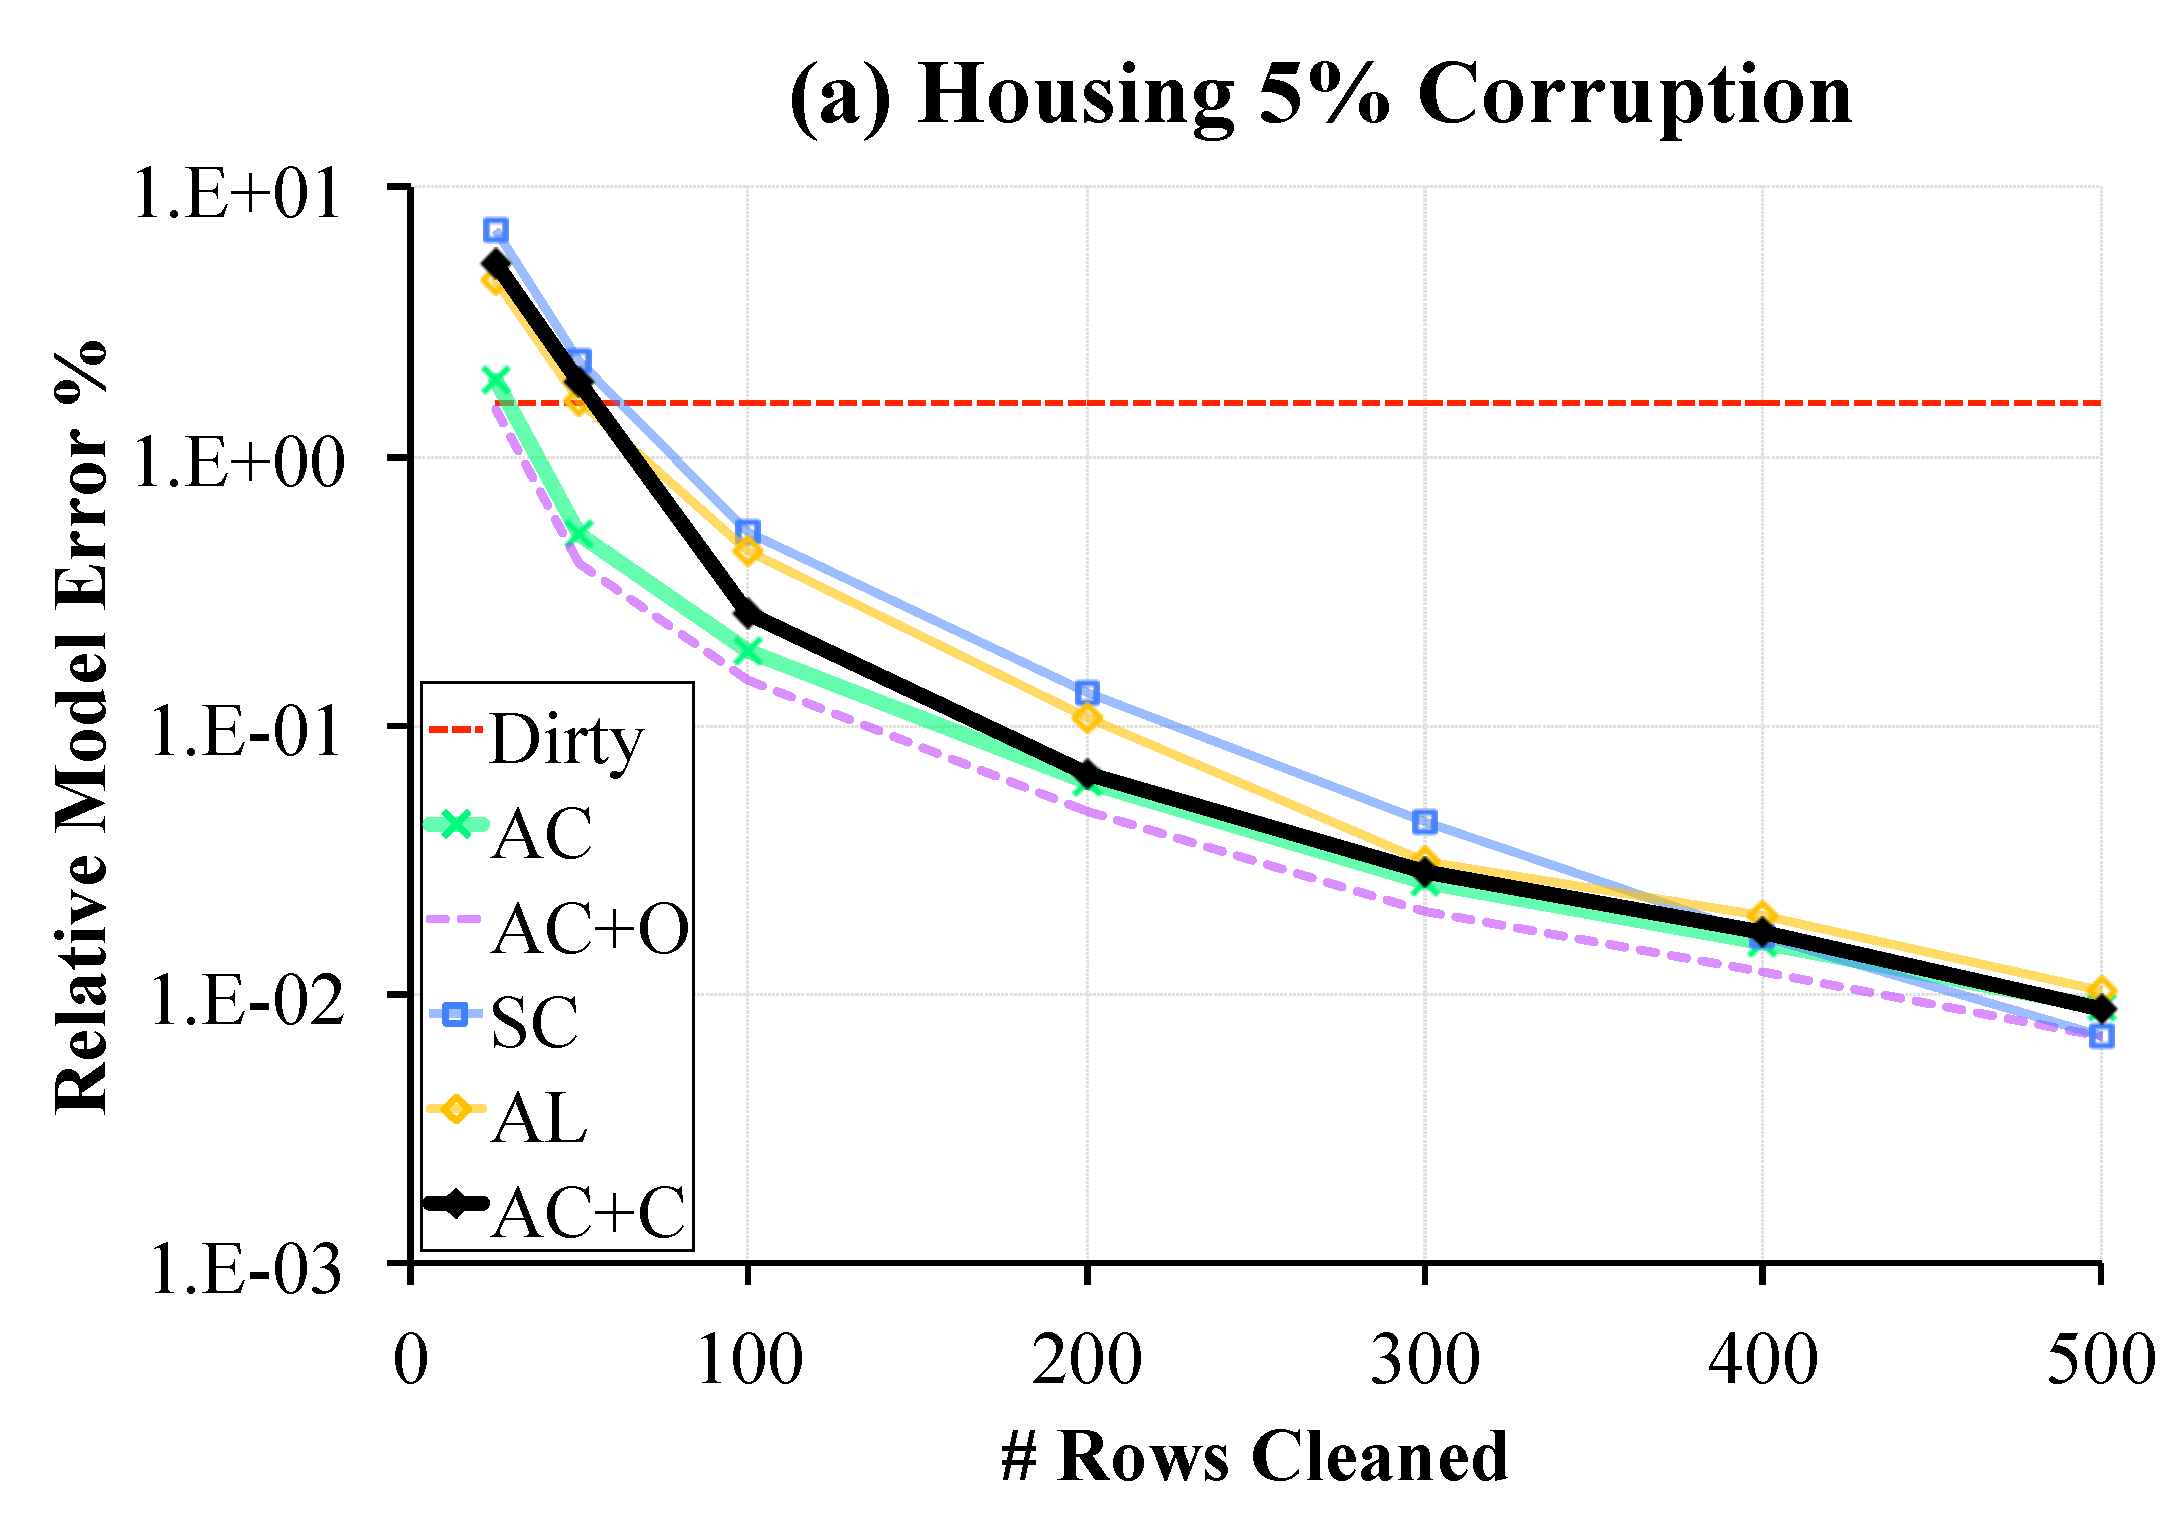
\includegraphics[width=0.48\columnwidth]{exp/exp11a.pdf}
 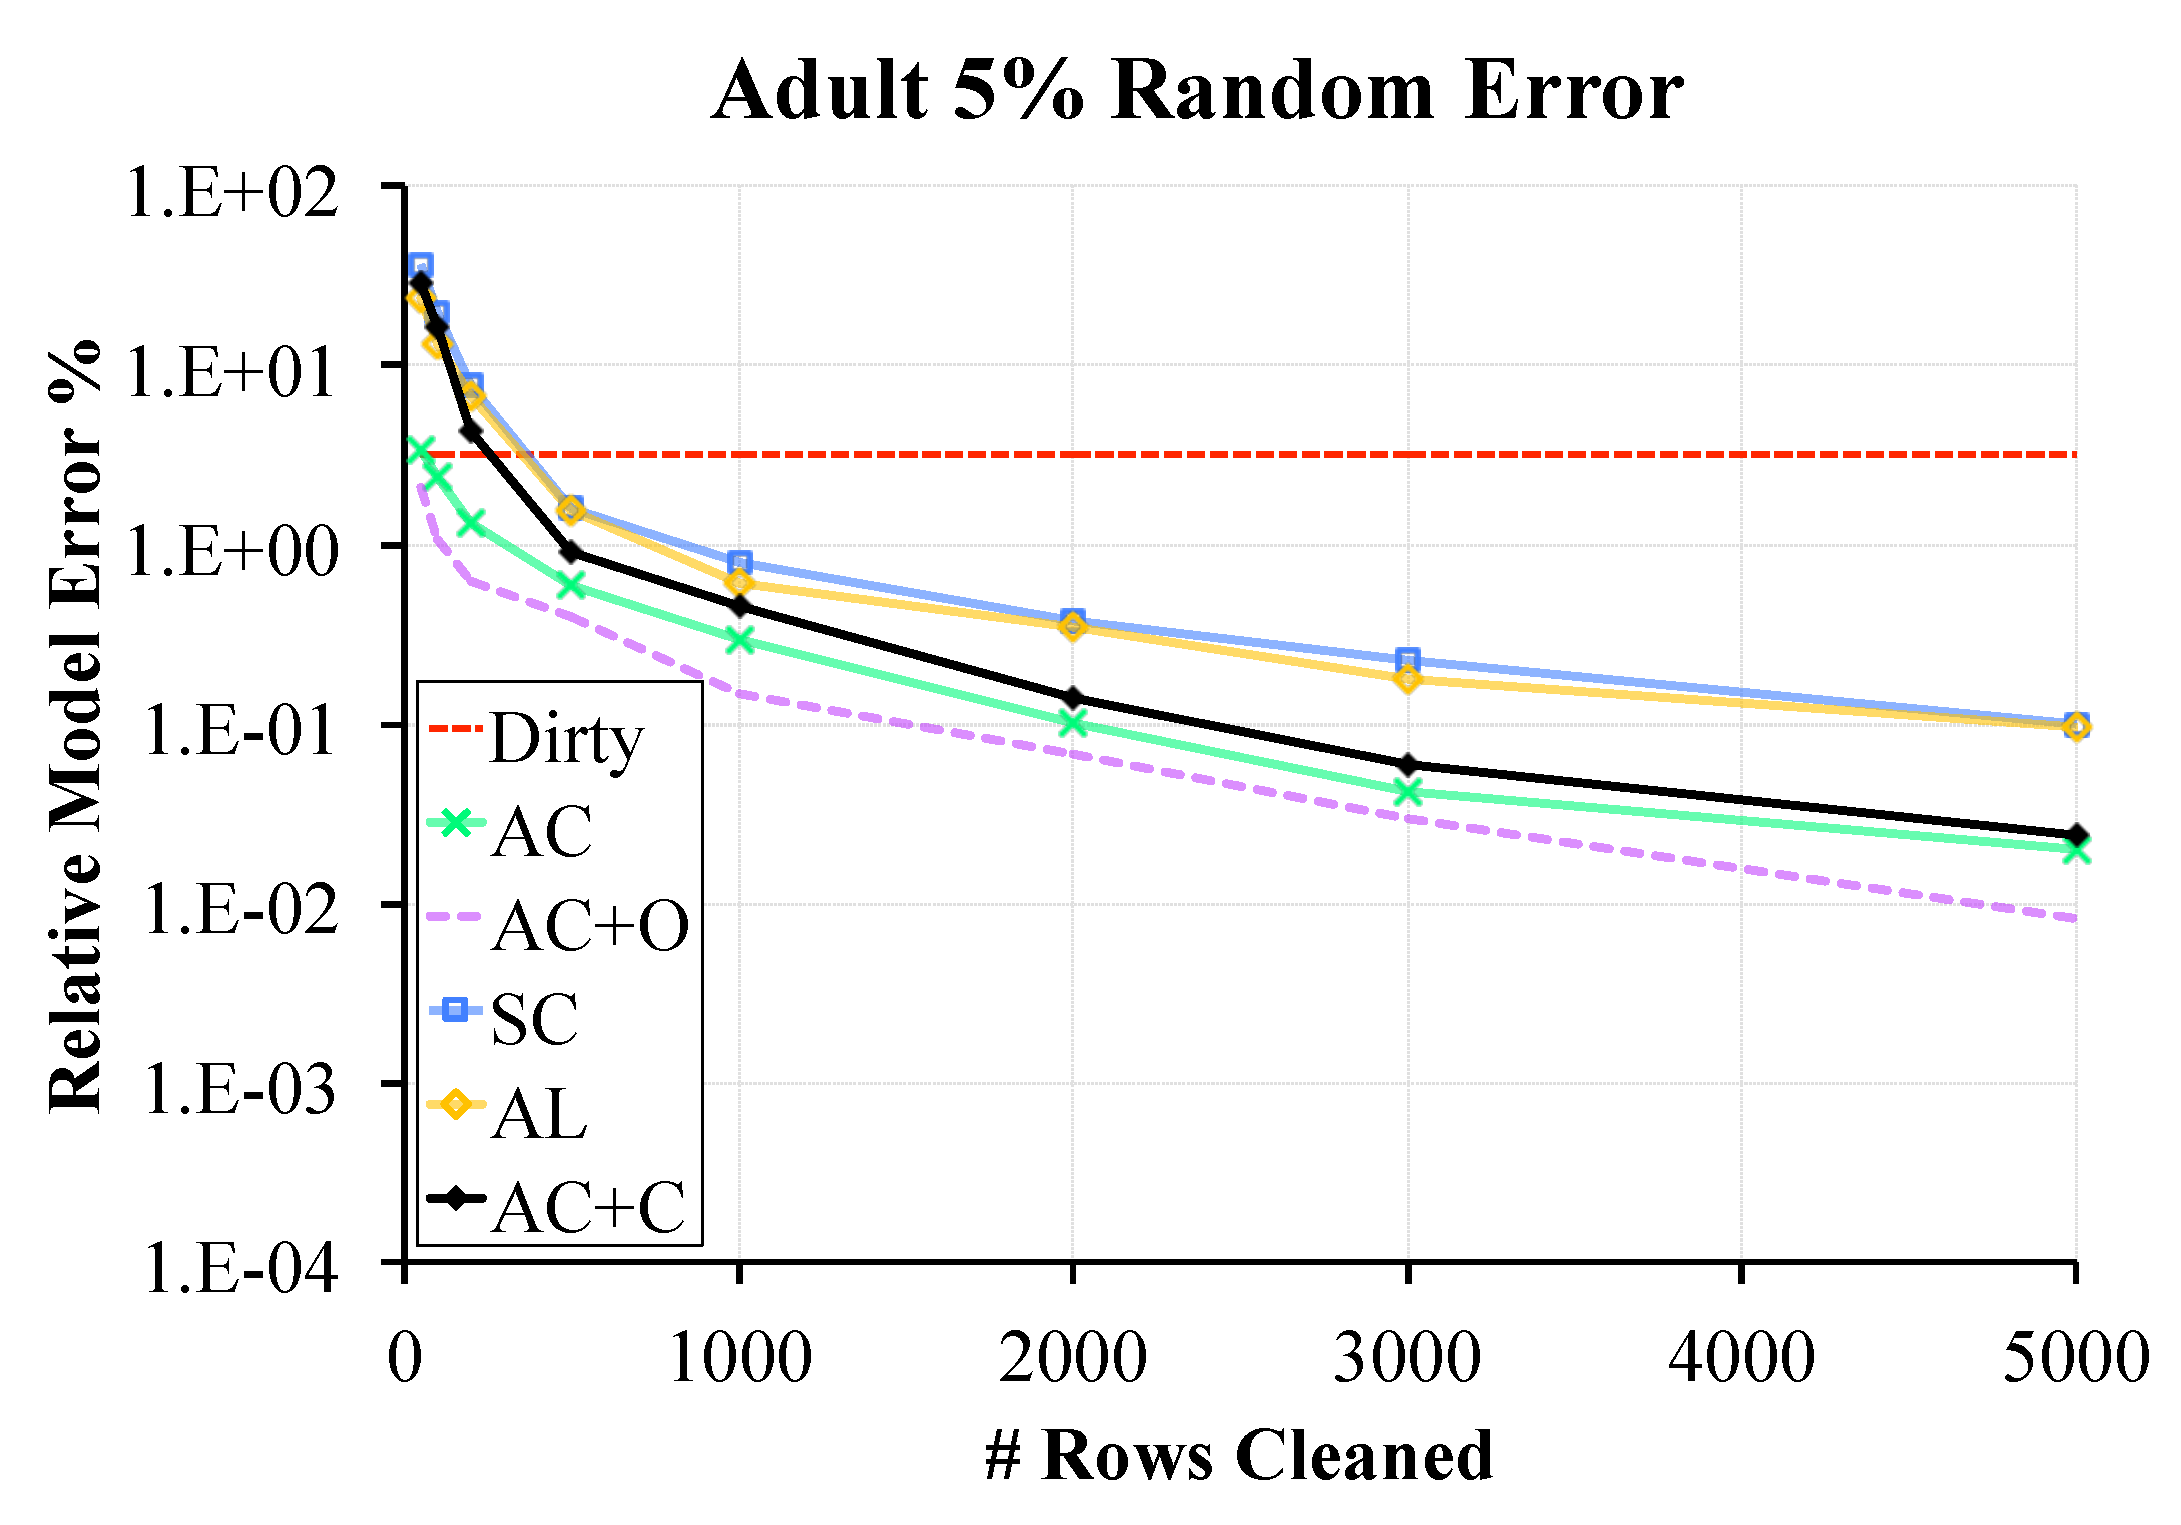
\includegraphics[width=0.48\columnwidth]{exp/exp11b.pdf}
 \caption{While initially \sys is comparable in performance to Active Learning, as the classifier improves, \sys converges faster than Active Learning and SampleClean. \label{pred-perf}}
\end{figure}

\subsubsection{3b. Classifiable Errors}
Using a classifier to partition errors depends on errors that can be classified.
For example, random errors that look like other data may be hard to learn.
As errors become more random, the classifier becomes increasingly erroneous.
We run an experiment where we start with the systematic errors described earlier.
With probability $p$, we increasingly make these errors more random.
We compare these results to AC-P where we do not partition the errors.
In Figure \ref{tradeoffs2}, we plot the error reduction using a classifier.
We find that when errors are about 40\% random then we reach a break even point
where the user is better of not partitiong the data since the errors introduced by incorrect classification are more than the error reductions.

\begin{figure}[ht!]
\centering
 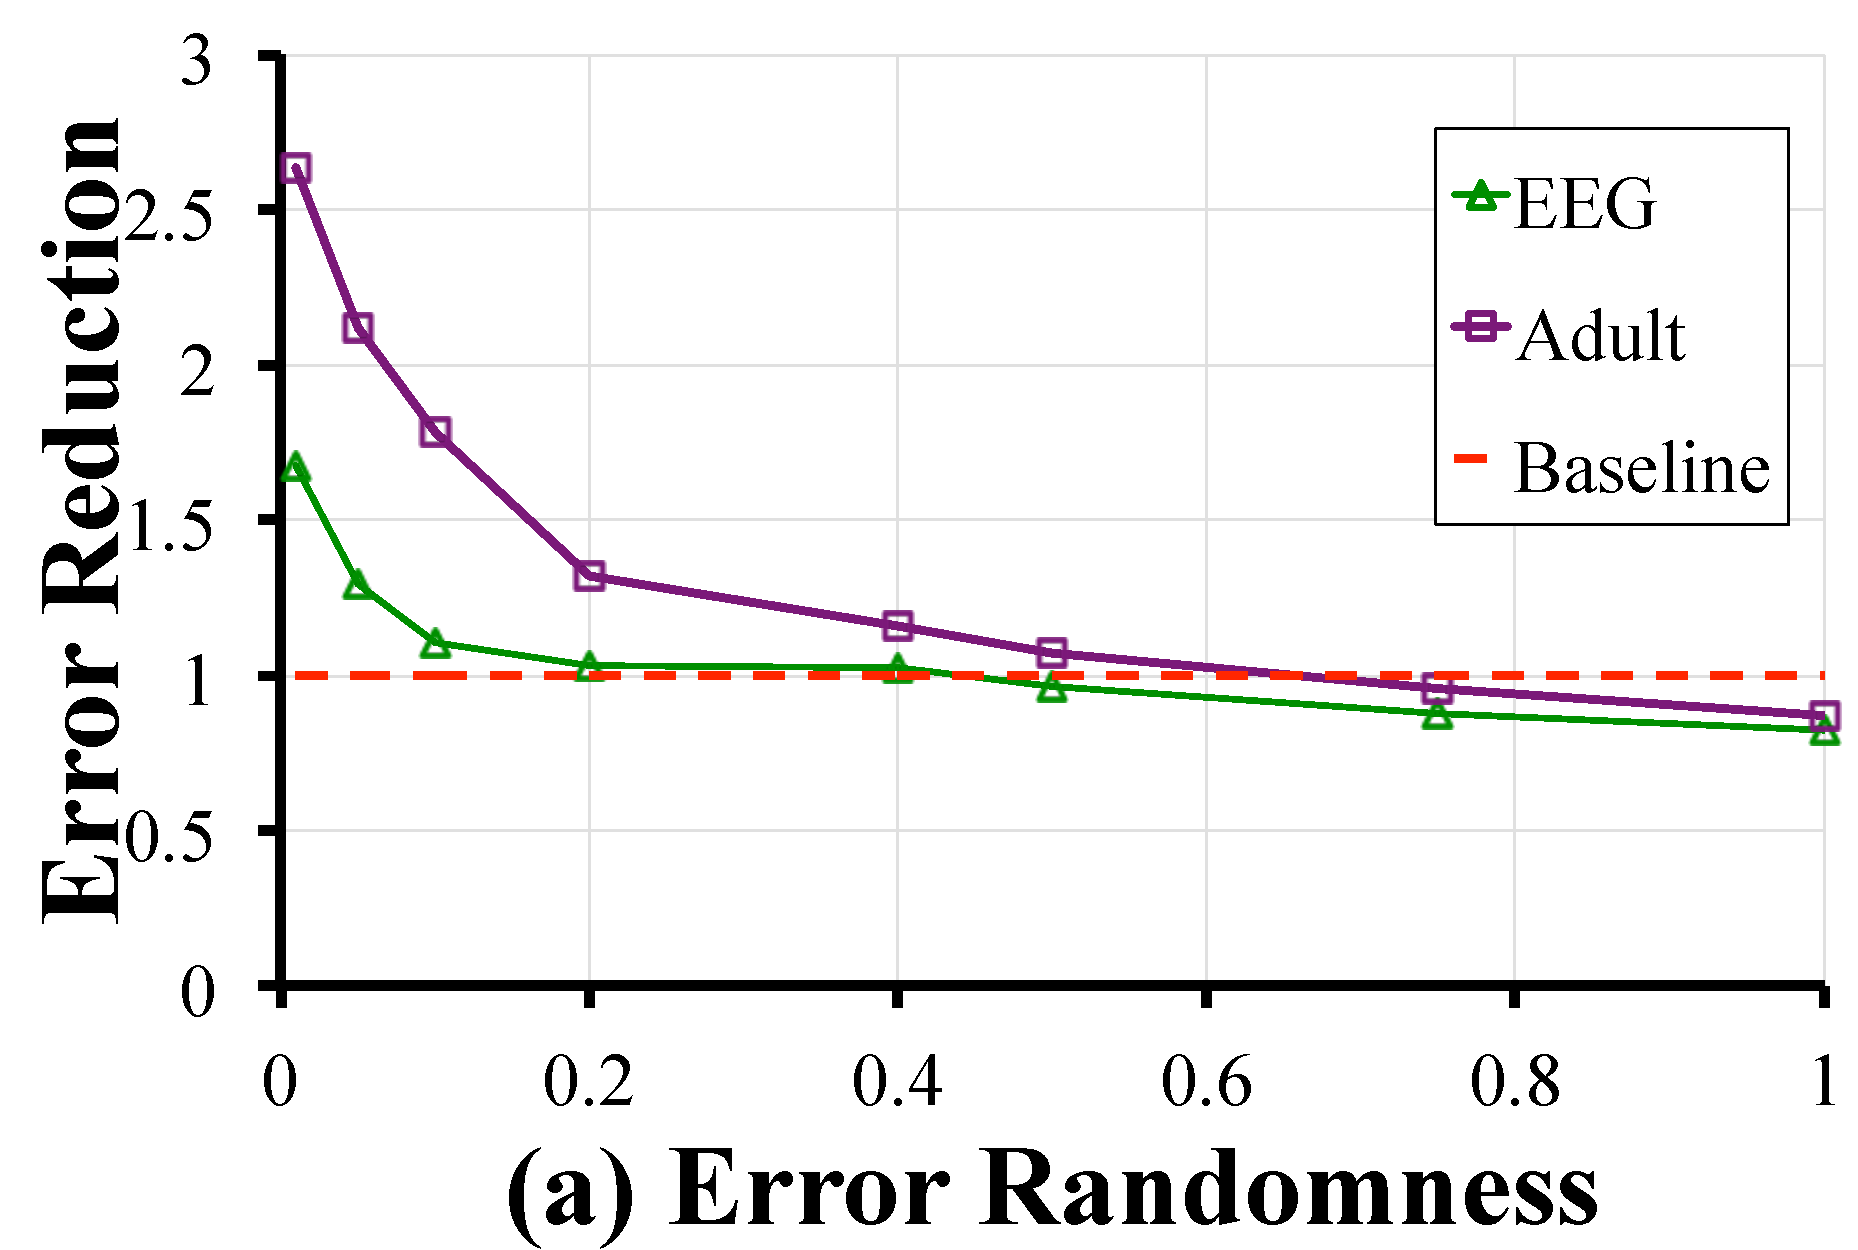
\includegraphics[scale=0.13]{exp/exp5a.pdf}
 \caption{Errors that are less random are easier to classify, and lead to more significant reductions in relative model error. \label{tradeoffs2}}
\end{figure}

\subsection{Experiment 4. Price of a Scan}
In our fourth set of experiments, we evaluate one of the computational premises of our work.
We argue that the price of a scan of data is cheap compared to data cleaning.
The overheads of partioning the dirty and clean data and calculating the sampling distribution should be small in comparison to the faster convergence of our model.
\reminder{How do we quantify the costs of data cleaning?} 

\subsection{Real Scenarios}
\reminder{Value Filling: MNIST}

\begin{figure*}[t]
\centering
 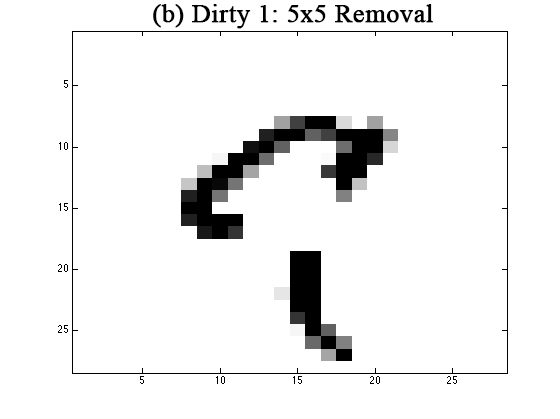
\includegraphics[scale=0.25]{exp/5x5removal.png}
 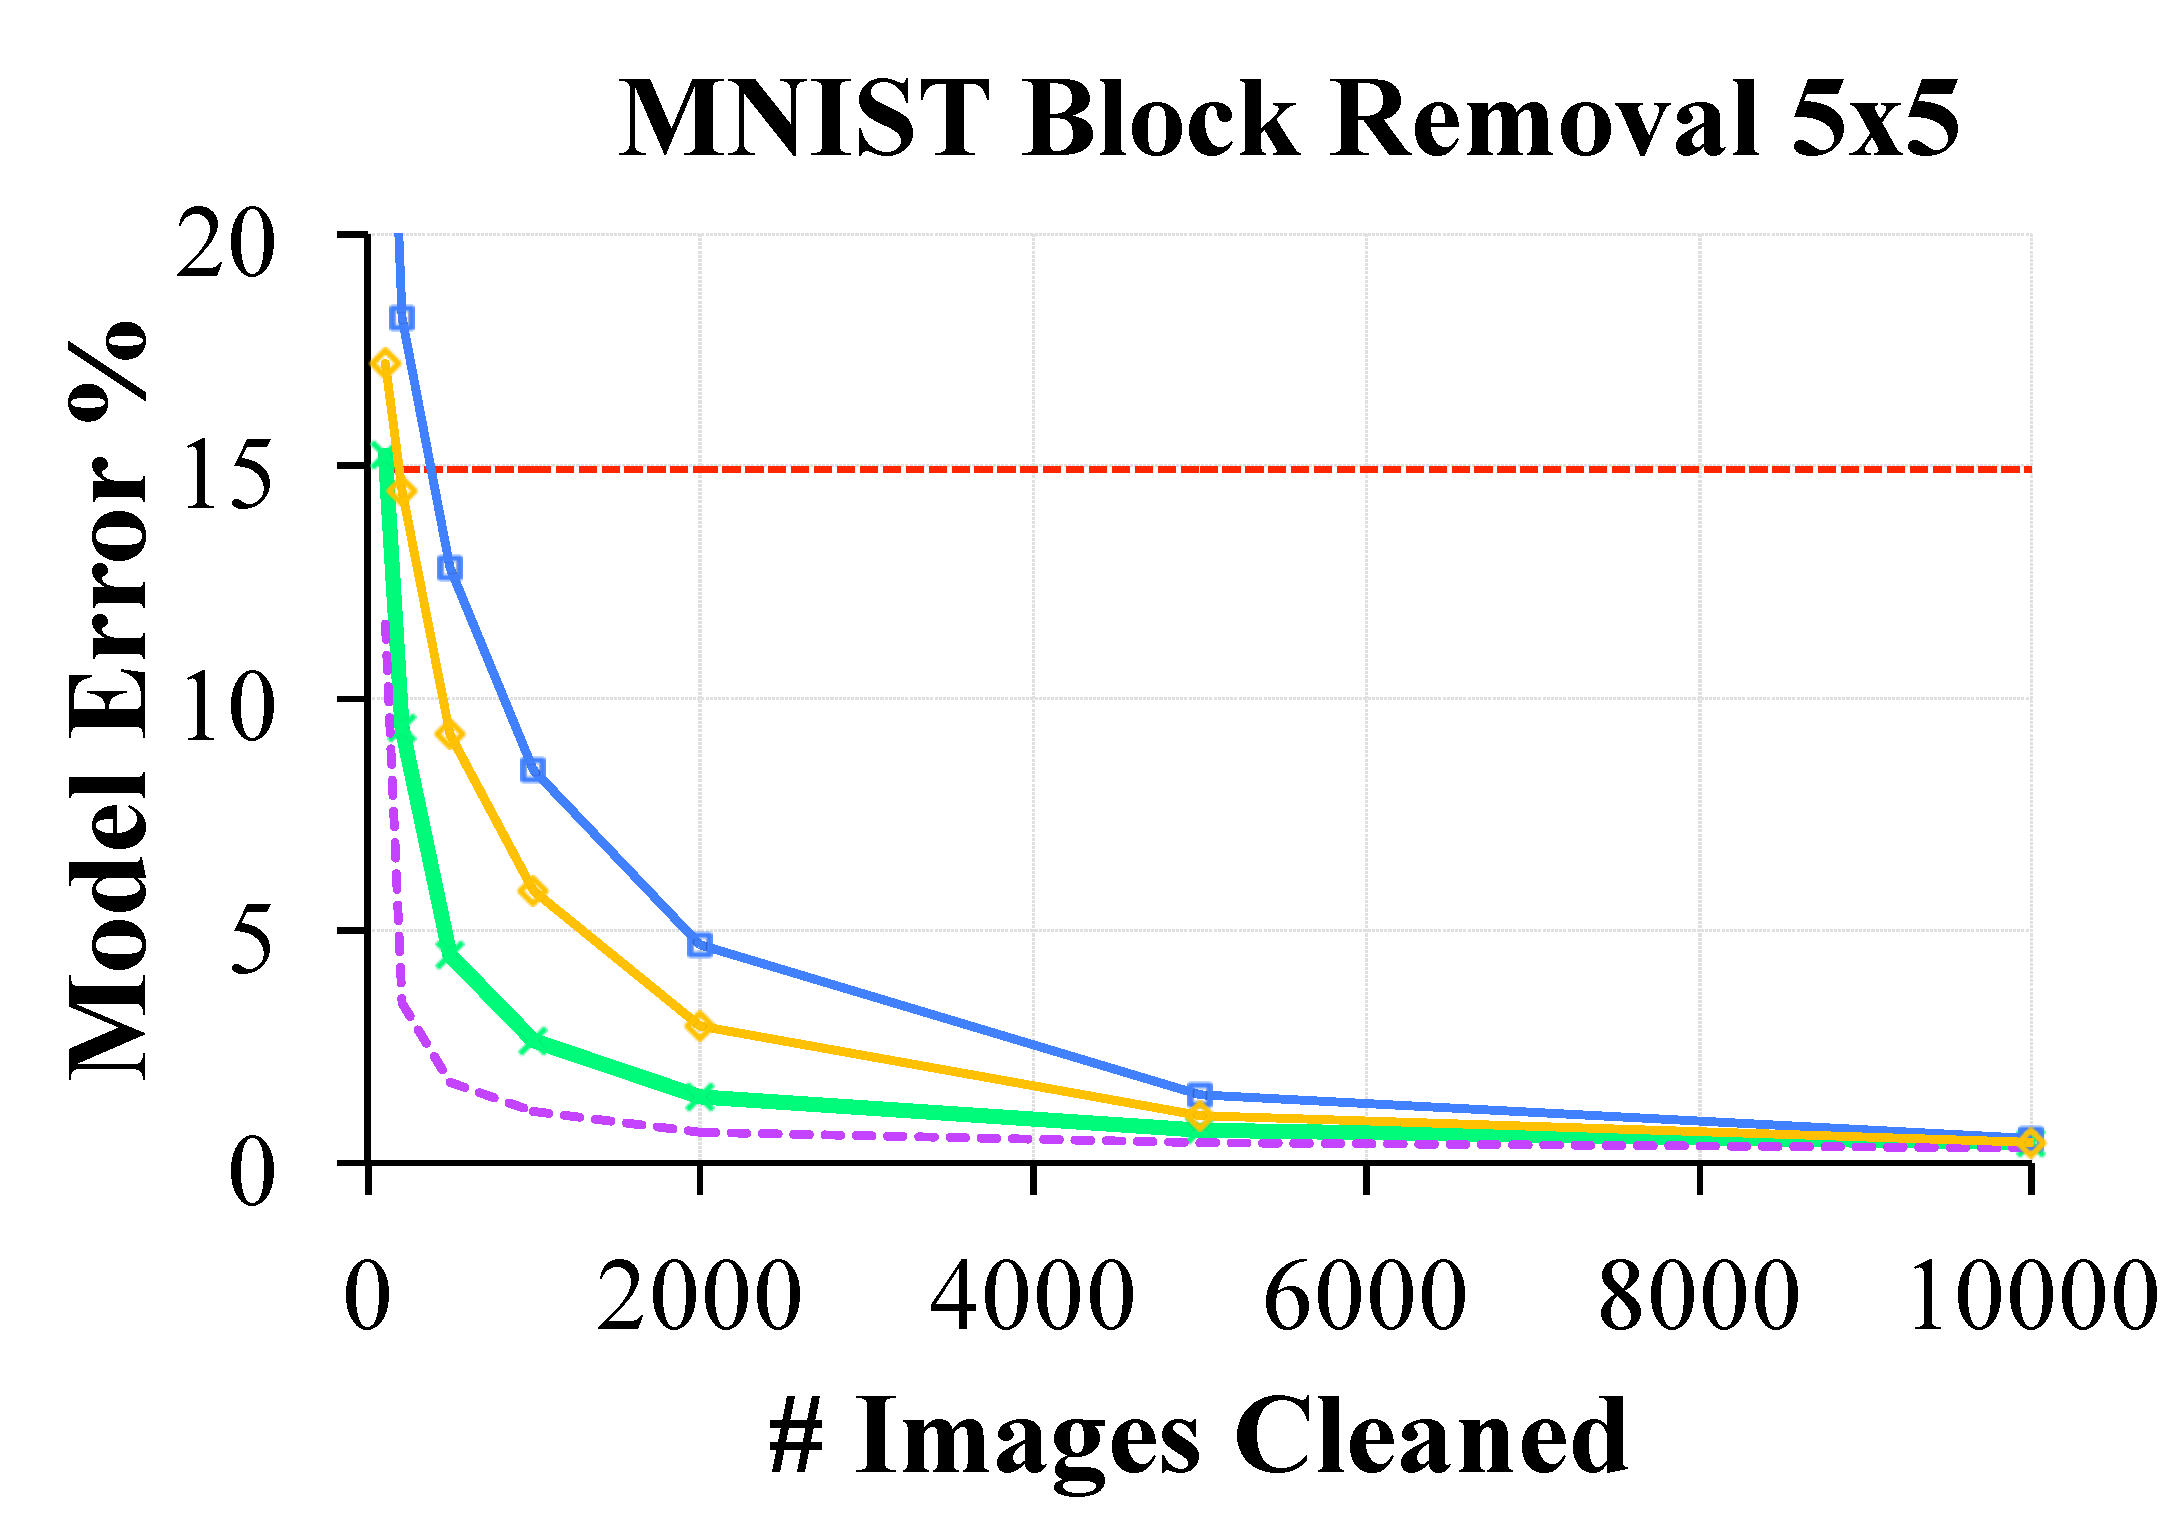
\includegraphics[scale=0.15]{exp/exp7a.pdf}
 \caption{One experiment with MNIST}
\end{figure*}

\reminder{CFD: Adult}
%
\section{Conclusion}
The growing popularity of predictive models (e.g., classifiers) in data analytics adds additional challenges in managing dirty data with mixing dirty and clean data, sensitivity to sampling, and sparsity.
\sys is a framework that utilizes data cleaning to mitigate systematic errors with progressive data cleaning.
The key insight is that an important class of predictive models, called convex loss models (e.g., linear regression and SVMs), can be simultaneously trained and cleaned.
Consequently, there are provable guarantees on the convergence and error bounds of \sys.  
\sys also includes numerous optimizations such as: using the information from the model to inform data cleaning on samples, dirty data detection to avoid sampling clean data, and batching together updates on already clean data.
The experimental results are promising as they suggest that these optimizations can significantly reduce data cleaning costs when errors are sparse and cleaning budgets are small.
Techniques such as Active Learning and SampleClean are not optimized for the sparse low-budget setting, and \sys achieves models of similar accuracy for significantly less records cleaned.
\vspace{-1em}

%\bibliographystyle{abbrv}
%\scriptsize
\fontsize{8.4pt}{8.7pt} \selectfont
\bibliographystyle{abbrv}
\bibliography{ref} 
\clearpage
\normalsize \selectfont
\appendix
%\section{Appendix}
\section{Set-of-Records Cleaning Model}\label{set-of-r}
In paper, we formalized the analyst-specified data cleaning as follows.
We take the sample of the records $S_{dirty}$, and apply data cleaning $C(\cdot)$.
$C$ is applied to a record and produces the clean record:
\[
S_{clean} = \{C(r) : \forall r \in S_{dirty}\}
\]
The record-by-record cleaning model is a formalization of the costs of data cleaning where each record has the same cost to clean and this cost does not change throughout the entire cleaning session.
There are, however, some cases when cleaning the first record of a certain type of corruption is expensive but all subsequent records are cheaper.

\begin{example}\label{app-ex1}
In most spell checking systems, when a misspelling is identified, the system gives an option to fix all instances of that misspelling.
\end{example}

\begin{example}\label{app-ex2}
In inconsistency problems, when an inconsistent value is identified all other records with the same inconsistency can be efficiently fixed.
\end{example}

This model of data cleaning can fit into our framework and we formalize it as the ``Set-of-Records" model as opposed to the ``Record-by-Record" model. 
In this model, the cleaning function $C(\cdot)$ is not restricted to updating only the records in the sample.
$C(\cdot)$ takes the entire dirty sample as an argument (that is the cleaning is a function of the sample), the dirty data, and updates the entire dirty data:
\[
R'_{dirty} = C(S_{dirty},R_{dirty})
\]
we require that for every record $s \in S_{dirty}$, that record is completely cleaned after applying $C(\cdot)$, giving us $S_{clean}$.
Records outside of $S_{dirty}$ may be cleaned on a subset of dirty attributes by $C(\cdot)$.
After each iteration, we re-run the detector, and move any $r \in R'_{dirty}$ that are clean to $R_{clean}$.
Such a model allows us to capture data cleaning operations such as in Example \ref{app-ex1} and Example \ref{app-ex2}.

\section{Stochastic Gradient Descent}\label{appsgd}

Stochastic Gradient Descent converges for a suitably chosen step size if the sample gradients are unbiased estimates of the full gradient. 
The first problem is to choose weights $\alpha$ and $\beta$ (to average already clean and newly cleaned data) such that the estimate of the gradient is unbiased. 
%SGD will converge when the estimate is unbiased and the step-size is chosen appropriately.
The batch $S_{dirty}$ is drawn only from $R_{dirty}$.
Since the sizes of $R_{dirty}$ and its complement are known, it follows that the gradient over the already clean data $g_C$ and the recently cleaned data $g_S$ can be combined as follows:
\[
g(\theta^{t}) = \frac{\mid R_{dirty} \mid \cdot g_S + \mid R_{clean} \mid \cdot g_C  }{\mid R \mid}
\]
Therefore,
\[
\alpha = \frac{\mid R_{clean} \mid}{\mid R \mid}, \beta = \frac{\mid R_{dirty} \mid}{\mid R \mid}
\]

\begin{lemma}
The gradient estimate $g(\theta)$ is unbiased if $g_S$ is an unbiased estimate of:
\[
\frac{1}{\mid R_{dirty} \mid} \sum g_i(\theta)
\]
\end{lemma}
\begin{proof}[Sketch]
\[
\mathbb{E}(\frac{1}{\mid R_{dirty} \mid} \sum g_i(\theta)) = \frac{1}{\mid R_{dirty} \mid} \cdot \mathbb{E}(\sum g_i(\theta)))
\]
By symmetry, 
\[
\mathbb{E}(\frac{1}{\mid R_{dirty} \mid} \sum g_i(\theta)) = g(\theta)
\]
\[
\mathbb{E}(\frac{1}{\mid R_{dirty} \mid} \sum g_i(\theta)) = \frac{\mid R_{dirty} \mid \cdot g_S + \mid R_{clean} \mid \cdot g_C  }{\mid R \mid}
\]
\end{proof}

The error bound discussed in Proposition 2 can be tightened for a class of models called strongly convex (see \cite{bertsekas2011incremental} for a defintion). 

\begin{proposition}
For a strongly convex loss, a batch size $b$, and $T$ iterations, the convergence rate is bounded by $O(\frac{\sigma^2}{bT})$. 
\end{proposition}

\section{Non-convex losses}\label{non-convex}
We acknowledge that there is an increasing popularity of non-convex losses in the Neural Network and Deep Learning literature. 
However, even for these losses, gradient descent techniques still apply. 
Instead of converging to a global optimum they converge to a locally optimal value. 
Likewise, \sys will converge to the closest locally optimal value to the dirty model. 
Because of this, it is harder to reason about the results.
Different initializations will lead to different local optima, and thus, introduces a complex dependence on the initialization with the dirty model.
This problem is not fundemental to \sys and any gradient technique suffers this challenge for general non-convex losses, and we hope to explore this more in the future.

\section{Importance Sampling}\label{impsample-deriv}
This lemma describes the optimal distribution over a set of scalars:
\begin{lemma}\label{impsample}
Given a set of real numbers $A = \{a_1,...,a_n\}$, let $\hat{A}$ be 
a sample with replacement of $A$ of size k.
If $\mu$ is the mean $\hat{A}$, the sampling distribution that minimizes
 the variance of $\mu$, i.e., the expected square error, is $p(a_i) \propto a_i$.
\end{lemma}
Lemma \ref{impsample} shows that when estimating a mean of numbers with sampling, the distribution with optimal variance is sampling proportionally to the values.

The variance of this estimate is given by:
\[
Var(\mu) = \mathbb{E}(\mu^2)-\mathbb{E}(\mu)^2
\] 
Since the estimate is unbiased, we can replace $\mathbb{E}(\mu)$ with the average of $A$:
\[
Var(\mu) = \mathbb{E}(\mu^2)-\bar{A}^2
\]
Since $\bar{A}$ is deterministic, we can remove that term during minimization.
Furthermore, we can write $\mathbb{E}(\mu^2)$ as:
\[
\mathbb{E}(\mu^2) = \frac{1}{n^2}\sum_i^n \frac{a_i^2}{p_i}
\]
Then, we can solve the following optimization problem (removing the proportionality of $\frac{1}{n^2}$) over the set of weights $P=\{p(a_i)\}$:
\[
\min_{P} \sum_i^N \frac{a_i^2}{p_i}
\]
\[
\text{subject to: } P > 0, \sum P = 1
\]
Applying Lagrange multipliers, an equivalent unconstrained optimization problem is:
\[
\min_{P > 0,\lambda > 0} \sum_i^N \frac{a_i^2}{p_i} + \lambda \cdot (\sum P - 1)
\]
If, we take the derivatives with respect to $p_i$ and set them equal to zero:
\[
-\frac{a_i^2}{2 \cdot p_i^2} + \lambda = 0
\]
If, we take the derivative with respect to $\lambda$ and set it equal to zero:
\[
\sum P - 1
\]
Solving the system of equations, we get:
\[
p_i = \frac{\mid a_i \mid }{\sum_i \mid a_i \mid}
\]

\section{Linearization}\label{apptaylor}
If $d$ is the dirty value and $c$ is the clean value, the Taylor series approximation for a function $f$ is given as follows:
\[
f(c) = f(d) + f'(d)\cdot(d-c) + ...
\]
Ignoring the higher order terms, the linear term $f'(d)\cdot(d-c)$ is a linear function in each feature and label.
We only have to know the change in each feature to estimate the change in value.
In our case the function $f$ is the gradient $\nabla\phi$.
So, the resulting linearization is:
\[
\nabla\phi(x^{(c)}_i,y^{(c)}_i,\theta) \approx \nabla\phi(x,y,\theta) + \frac{\partial}{\partial X}\nabla\phi(x,y,\theta)\cdot (x - x^{(c)}) \]
\[+ \frac{\partial}{\partial Y}\phi(x,y,\theta)\cdot (y - y^{(c)})
\]
When we take the expected value:
\[
\mathbb{E}(\nabla\phi(x_{clean},y_{clean},\theta)) \approx \nabla\phi(x,y,\theta) + \frac{\partial}{\partial X}\nabla\phi(x,y,\theta)\cdot \mathbb{E}(\Delta x) \]
\[+ \frac{\partial}{\partial Y}\nabla\phi(x,y,\theta)\cdot \mathbb{E}(\Delta y)
\]
It follows that:
\[
\approx \nabla\phi(x,y,\theta) + M_x \cdot \mathbb{E}(\Delta x) + M_y \cdot \mathbb{E}(\Delta y)
\]
where $M_x = \frac{\partial}{\partial X}\nabla\phi$ and $M_y = \frac{\partial}{\partial Y}\nabla\phi$.
Recall that the feature space is $d$ dimensional and label space is $l$ dimensional.
Then, $M_x$ is an $d \times d$ matrix, and $M_y$ is a $d \times l$ matrix.
Both of these matrices are computed for each record.
$\Delta x$ is a $d$ dimensional vector where each component represents a change in that feature and $\Delta y$ is an $l$ dimensional vector that represents the change in each of the labels. 

This linearization allows \sys to maintain per feature (or label) average changes and use these changes to center the optimal sampling distribution around the expected clean value.
To estimate $\mathbb{E}(\Delta x)$ and $\mathbb{E}(\Delta y)$, consider the following for a single feature $i$:
If we average all $j=\{1,...,K\}$ records cleaned that have an error for that feature, weighted by their sampling probability:
\[
\bar{\Delta}_{xi} = \frac{1}{NK}\sum_{j=1}^K (x^{(d)}[i]-x^{(c)}[i])\times \frac{1}{p(j)}
\]
Similarly, for a label $i$:
\[
\bar{\Delta}_{yi} = \frac{1}{NK}\sum_{j=1}^K (y^{(d)}[i]-y^{(c)}[i])\times \frac{1}{p(j)}
\]

Each $\bar{\Delta}_{xi}$ and $\bar{\Delta}_{yi}$ represents an average change in a single feature.
A single vector can represent the necessary changes to apply to a record $r$:
For a record $r$, the set of corrupted features is $f_r,l_r$.
Then, each record $r$ has a d-dimensional vector $\Delta_{rx}$ which is constructed as follows:
\[
 \Delta_{rx}[i] = \begin{cases} 0 & i \notin f_r \\ 
\bar{\Delta}_{xi} & i \in f_r
\end{cases} 
\]
Each record $r$ also has an l-dimensional vector $\Delta_{ry}$ which is constructed as follows:
\[
 \Delta_{rx}[i] = \begin{cases} 0 & i \notin l_r \\ 
\bar{\Delta}_{yi} & i \in l_r
\end{cases} 
\]
Finally, the result is: 
\[p_{r}\propto\|\nabla\phi(x,y,\theta^{(t)}) + M_x \cdot \Delta_{rx} +  M_y \cdot \Delta_{ry}\|
\]

\section{Example $M_x$, $M_y$}\label{example-deriv}
\noindent\textbf{Linear Regression: }
\[
\nabla\phi(x,y,\theta) = (\theta^Tx - y)x
\]
For a record, $r$, suppose we have a feature vector $x$.
If we take the partial derivatives with respect to x, $M_x$ is:
\[
M_x[i,i] = 2x[i] + \sum_{i \ne j} \theta[j]x[j] - y 
\]
\[
M_x[i,j] = \theta[j]x[i]
\]
Similarly $M_y$ is:
\[
M_y[i,1] = x[i] 
\]

\vspace{0.5em}

\noindent\textbf{Logistic Regression: } 
\[
\nabla\phi(x,y,\theta) = (h(\theta^Tx) - y)x
\]
where
\[
h(z) = \frac{1}{1+e^{-z}}
\]
we can rewrite this as:
\[
h_{\theta}(x) = \frac{1}{1+e^{\theta^Tx}}
\]
\[
\nabla\phi(x,y,\theta) = (h_{\theta}(x) - y)x
\]
In component form,
\[
g = \nabla\phi(x,y,\theta)
\]
\[
g[i] = h_{\theta}(x)\cdot x[i] - yx[i]
\]
Therefore,
\[
M_x[i,i] = h_{\theta}(x)\cdot(1- h_{\theta}(x))\cdot \theta[i] x[i] + h_{\theta}(x) - y
\]
\[
M_x[i,j] = h_{\theta}(x)\cdot(1- h_{\theta}(x))\cdot \theta[j] x[i] + h_{\theta}(x)
\]
\[
M_y[i,1] = x[i] 
\]

\noindent\textbf{SVM: } 
\[
\nabla\phi(x,y,\theta) =
\begin{cases}      
-y\cdot\boldsymbol{x} \text{ if } y\cdot\boldsymbol{x}\cdot\theta \le 1 \\
0\ \text{ if } y\ \boldsymbol{x}\cdot\theta \geq 1      
\end{cases}
\]
Therefore,
\[
M_x[i,i] = \begin{cases}      
-y[i] \text{ if } y\cdot\boldsymbol{x}\cdot\theta \le 1 \\
0\ \text{ if } y\ \boldsymbol{x}\cdot\theta \geq 1      
\end{cases} 
\]
\[
M_x[i,j] = 0
\]
\[
M_y[i,1] = x[i] 
\]

\section{Aggregate Queries as Convex Losses}
\subsection{AVG and SUM queries}
\avgfunc, \sumfunc queries are a special case of the convex loss minimization discussed in the paper:
If we define the following loss, it is easy to verify the the optimal $\theta$ is the mean $\mu$:
\[
\phi = (x_{i} - \theta)^2
\]
with the appropriate scaling it can support $\avgfunc$, $\sumfunc$ queries with and without predicates.
Taking the gradient of that loss:
\[
\nabla\phi = 2(x_{i} - \theta)
\]
It is also easy to verify that the bound on errors is $O(\frac{\mathbb{E}((x-\mu)^2}{bT})$, which is essentially the CLT.
The importance sampling results are inutitive as well.
Applying the linearization:
\[
M_x = 2
\]
The importance sampling prioritizes points that it expects to be far away from the mean.

\subsection{MEDIAN}
Similarly, we can analyze the \medfunc query.
If we define the following loss, it is easy to verify the the optimal $\theta$ is the median $m$:
\[
\phi = \mid x_{i} - \theta\mid
\]
Taking the gradient of that loss:
\[
\nabla\phi = \text{1 if < m, -1 if > m}
\]
Applying the linearization:
\[
M_x = 0
\]
The intuitive result is that a robust query like a median does not need to consider estimation as the query result is robust to small changes.

\section{Experimental Comparison}
\subsection{Robust Logistic Regression}\label{rlogit}
We use the algorithm from Feng et al. for robust logistic regression.
\begin{enumerate}
\item Input: Contaminated training samples $\{(x_1, y_1), . . . ,(x_{n}
, y_{n})\}$ an upper bound on the number of outliers n, number of inliers n and sample dimension p.
\item Initialization: Set \[T = 4\sqrt{\log p/n + \log n/n}\]
\item Remove samples $(xi
, yi)$ whose magnitude satisfies $\|x_i\| \ge T$.
\item Solve regularized logistic regression problem.
\end{enumerate}

\subsection{Active Learning}\label{al}
There is a well established link between Active Learning and Online Gradient-based Algorithms \cite{guillory2009active}. 
To fairly evaluate an Active Learning methodology in these experiments, we run a gradient descent where examples are priortized by expected gradient length (explained in \cite{settles2010active}).
Ignoring the detection step, there are two differences between this algorithm and the one we propose.
First, we calculate the gradient with respect to the an estimate of the clean data, and second we sample rather than using a deterministic ordering.
While such Active Learning algorithms have been studied in the Learning Theory community, they have not been adopted in data cleaning or crowdsourcing research.
Typical algorithms include uncertainty sampling, where a classifier prioritized data closest to the margin.
However, algorithms such as uncertainty sampling focus on the narrow problem of label acquisition in hyperplane classifiers; a problem too narrow for application in this setting.

\section{Dollars For Docs Setup}\label{dfd-errors}
The dollars for docs dataset has the following schema:
\begin{lstlisting}[mathescape,basicstyle={\scriptsize}]
Contribution(pi_speciality$\textrm{,}$ drug_name$\textrm{,}$ device_name$\textrm{,}$
corporation$\textrm{,}$ amount$\textrm{,}$ dispute$\textrm{,}$ status)
\end{lstlisting}
To flag suspect donations, we used the \texttt{status} attribute.
When the \texttt{status} was ``covered" that means it was an allowed contribution under the researcher's declared protocol.
When the \texttt{status} was ``non-covered" that means it was a disallowed contribution under the researcher's declared protocol.
The rest of the textual attributes were featurized with a bag-of-words model, and the numerical amount and dispute attributes were treated as numbers.

We cleaned the entire Dollars for Docs dataset upfront to be able to evaluate how different budgeted data cleaning strategies compare to cleaning the full data.
To clean the dataset, we loaded the entire data 240089 records into Microsoft Excel. We identified four broad classes of errors:
\vspace{0.25em}

\noindent \textbf{Corporations are inconsistently represented: } ``Pfizer", ``Pfizer Inc.", ``Pfizer Incorporated".

\vspace{0.25em}

\noindent \textbf{Drugs are inconsistently represented: } ``TAXOTERE  DOCETAXEL -PROSTATE CANCER" and ``TAXOTERE"

\vspace{0.25em}

\noindent \textbf{Label of covered and not covered are not consistent: } ``No", ``Yes",``N", ``This study is not supported", ``None", ``Combination"

\vspace{0.25em} 

\noindent \textbf{Research subject must be a drug OR a medical device and not both: } ``BIO FLU QPAN H7N9AS03 Vaccine" and ``BIO FLU QPAN H7N9AS03 Device"

\vspace{0.5em} 

To fix these errors, we sorted by each column and merged values that looked similar and removed inconsistencies as in the status labels. 
When there were ambiguities, we refered to the drug company's website and whitepapers.
When possible, we used batch data transformations, like find and replace (i.e. the Set-of-Records model).
In all, 44234 records had some error and full data cleaning required about 2 days of efforts.

Once cleaned, in our experiment, we encoded the 4 problems as data quality constraints.
To fix the constraints, we looked up the clean value in the dataset that we cleaned up front.

\vspace{0.25em}

\noindent \textbf{Rule 1: } Matching dependency on corporation (Weighted Jaccard Similarity $>$ 0.8).

\vspace{0.25em}

\noindent \textbf{Rule 2: } Matching dependency on drug (Weighted Jaccard Similarity $>$ 0.8).

\vspace{0.25em}

\noindent \textbf{Rule 3: } Label must either be ``covered" or ``not covered".

\vspace{0.25em} 

\noindent \textbf{Rule 4: } Either drug or medical device should be null.

\vspace{0.5em}

\section{MNIST Setup}
We include visualization of the errors that we generated for the MNIST experiment.
We generated these errors in MATLAB by taking the grayscale version of the image (a $64\times 64$ matrix) and corrupting them by block removal and fuzzying.

\begin{figure}[ht]
\centering
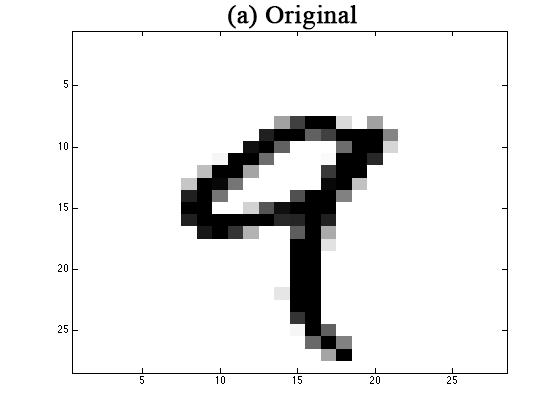
\includegraphics[scale=0.20]{exp/original.png}
 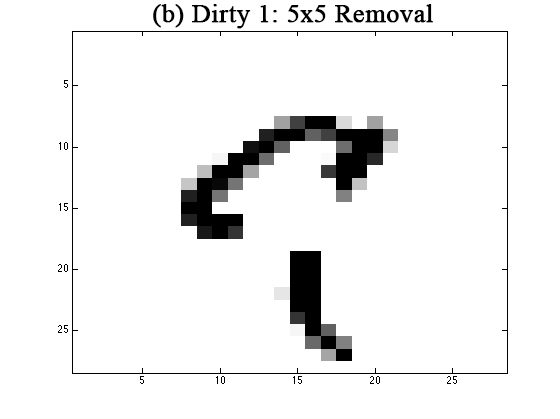
\includegraphics[scale=0.20]{exp/5x5removal.png}
 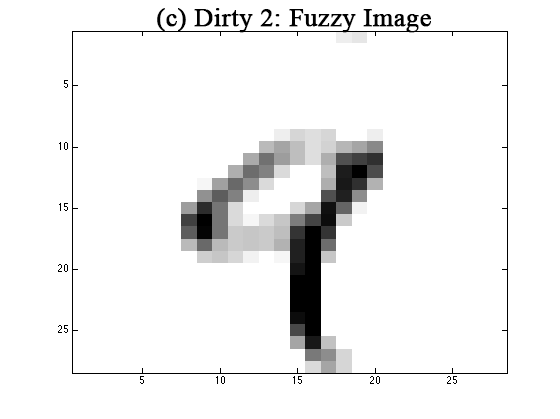
\includegraphics[scale=0.20]{exp/fuzzy.png}
 \caption{We experiment with two forms of corruption in the MNIST image datasets: 5x5 block removal and making the images fuzzy. Image (a) shows an uncorrupted ``9", image (b) shows one corrupted with block removal, and image (c) shows one that is corrupted with fuzziness. \label{mnist-corr}}
\end{figure}

\end{document}